\documentclass{article}
\usepackage{amssymb}
\usepackage{graphicx}
\usepackage{caption}
\usepackage{subcaption}
\usepackage{listings}
\usepackage{float} %figure inside minipage
\graphicspath{ {./images/} }
\usepackage[export]{adjustbox}
\usepackage{cite}
\usepackage{amsmath}
\usepackage{hyperref}

% gives the \cites command for multiple citations
\makeatletter
\newcommand{\citecomment}[2][]{\citen{#2}#1\citevar}
\newcommand{\citeone}[1]{\citecomment{#1}}
\newcommand{\citetwo}[2][]{\citecomment[,~#1]{#2}}
\newcommand{\citevar}{\@ifnextchar\bgroup{;~\citeone}{\@ifnextchar[{;~\citetwo}{]}}}
\newcommand{\citefirst}{\@ifnextchar\bgroup{\citeone}{\@ifnextchar[{\citetwo}{]}}}
\newcommand{\cites}{[\citefirst}
\makeatother

\begin{document}
\begin{titlepage}
\author{Humaid Agowun and Paul Muir} 
\title{Efficient defect control for IVODES based on multistep Hermite-Birkhoff interpolants
} 
\date{\today} 
\maketitle
\end{titlepage}

\begin{center}
    \textbf{Abstract}
\end{center}

In this report, we consider the concept of `defect control'. We discuss its importance and the efficiency issues associated with ODE solvers based on Runge-Kutta methods \cite{MR3822086} that control the maximum defect of a continuous approximate solution. Standard approaches typically makes use of continuous Runge-Kutta methods \cite{MR3822086} to perform defect control which typically involves performing several evaluations of the right hand side function of the ODE, $f(t, y(t))$. In this chapter, we consider an approach to perform defect control using a multistep Hermite interpolant \cite{MR3822086} that requires no additional function evaluations. We will augment $4^{th}$, $6^{th}$ and $8^{th}$ order Runge Kutta methods with a Hermite cubic, with a sixth order Hermite-Birkhoff interpolant and an eighth order Hermite-Birkhoff interpolant and show that high quality interpolants can be obtained using no extra function evaluations. In its simplest form, a numerical method typically solves an ODE by stepping from the initial time to the final time, using stepsize $h$. It computes a solution approximation at the end of each step. A method is said to be of order $p$, if the error associated with the solution approximations it computes behaves like O($h^p$). We will discuss challenges associated with this approach and how these challenges can be addressed. We then conclude with suggestions for additional work that can be done on this project.



\section{Introduction}

In this chapter, we present an efficient defect control technique for use in the numerical solution of initial value ordinary differential equations (ODE). We will assume that the underlying numerical method is a Runge-Kutta (RK) method since the vast majority of the literature on the use of defect control for numerical solution of IVODEs focuses on RK methods. Solvers based on Runge-Kutta methods only provide a discrete numerical solution. They adaptively divide the time domain into steps and return an estimate of the solution at the end of each step. To get a continuous solution approximate, the user has to fit an interpolant over the whole region.

The issue is that there is no guarantee that the interpolant will be as accurate as the discrete solution calculated by the solver. Thus if the solver returned a solution that satisfied a tolerance of $10^{-i}$, there are no guarantee that in the middle of a step, the interpolant will also deliver approximate solution values whose accuracy is approximately $10^{-i}$. 

High quality contemporary IVODE solvers typically have a built-in interpolant that provides a continuous solution approximation. However the solvers typically do not provide any type of explicit control of the accuracy of the continuous solution approximate. We show in Section $\ref{section:end_of_step_innacurate}$, that even for the robust IVODE solvers in Python, using interpolation does not guarantee solution approximations that have the same accuracy as the solution approximations at the end of each step. 


There has been some work towards addressing this issue in the area of control of the defect of the continuous solution approximation \cites{MR2600928}{MR1950917}{MR1803189}{MR1239829}{MR997658}{MR996053}. The defect is the amount by which the continuous solution approximation fails to satisfy the IVODE. We discuss this work in Section $\ref{section:crk_related_work}$. Typically, the interpolants employed in algorithms for defect control are based on the use of Continuous Runge-Kutta methods and the computational costs are substantial. 

In this paper we will discuss an efficient method for defect control of the continuous solution using multistep Hermite Birkhoff interpolants. For related work, see \cites{MR1239829}{tsitouras1990runge}{papageorgiou1997continuous} and the references within. We will control an estimate of the maximum defect along a step and show how that yields a continuous solution approximation over the whole time domain whose defect is typically within the tolerance.

We start by discussing the ODE problems we will use to demonstrate our approach in Section $\ref{section:defect_problem_used}$. We then give an overview of the issue with using error control only at the end of the step in Section $\ref{section:end_of_step_innacurate}$. We discuss related work in Section $\ref{section:crk_related_work}$. We give a description of the solvers that we use in Section $\ref{section:basic_runge_kutta}$. 

We discuss several multistep interpolants that we have constructed based on a Runge-Kutta method of order 4 in Section $\ref{section:equipping_rk4_with_HBs}$ and extend them to higher order Runge-Kutta methods in Section $\ref{section:HBs_and_higher_order_RK}$. We then discuss possible solutions to a fundamental issue with our approach in Section $\ref{section:keeping_alpha_at_1}$ and give some final recommendations on building a final solver in Section $\ref{section:defect_final_recommendations}$.

\subsection{Test Problems}
\label{section:defect_problem_used}
In this section, we discuss the three problems that we use \cite{MR1421071}. 

The first problem has the ODE:
\begin{equation}
y'(t) = - \frac{y^{3}(t)}{2} 
\end{equation}
The initial condition is $y(0) = 1$ and the time domain is $[0, 10]$.

The solution to this problem is
\begin{equation}
y(t) = \frac{1}{\sqrt{1 + t}}.
\end{equation}
as shown in Figure $\ref{fig:solution_problem1}$.

\begin{figure}[H]
\centering
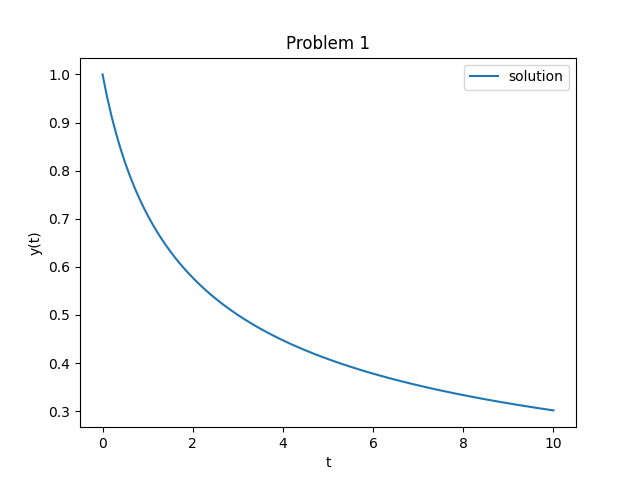
\includegraphics[width=0.7\linewidth]{./figures/solution_problem1}
\caption{Solution to the first ODE problem.}
\label{fig:solution_problem1}
\end{figure}

The second problem has the ODE:
\begin{equation}
y'(t) = \frac{y(t)(1 - \frac{y(t)}{20})}{4}.
\end{equation}
The initial condition is $y(0) = 1$ and the time domain is $[0, 10]$.

The solution to this problem is
\begin{equation}
y(t) = \frac{20e^{\frac{t}{4}}}{e^{\frac{t}{4}} + 19},
\end{equation}
as shown in Figure $\ref{fig:solution_problem2}$.

\begin{figure}[H]
\centering
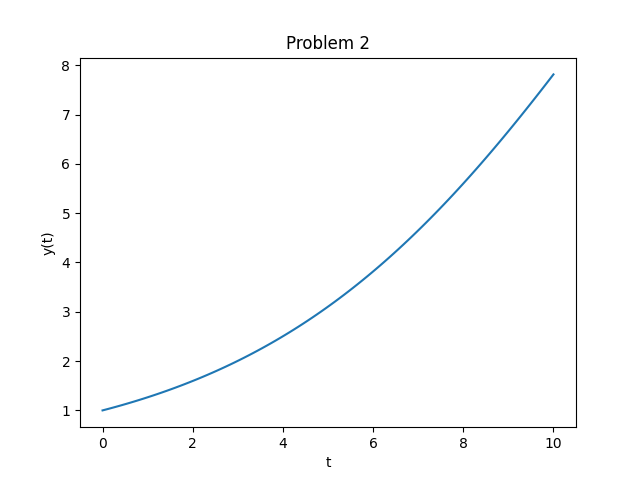
\includegraphics[width=0.7\linewidth]{./figures/solution_problem2}
\caption{Solution to the second ODE problem.}
\label{fig:solution_problem2}
\end{figure}

The third problem has the ODE:
\begin{equation}
y'(t, y) = -0.1y - e^{-0.1t}\sin(t)
\end{equation}
The initial condition is $y(0) = 1$ and the time domain is $[0, 10]$.

The solution to this problem is 
\begin{equation}
y(t) = e^{-0.1t}\cos(t),
\end{equation}
as shown in Figure $\ref{fig:solution_problem3}$.

\begin{figure}[H]
\centering
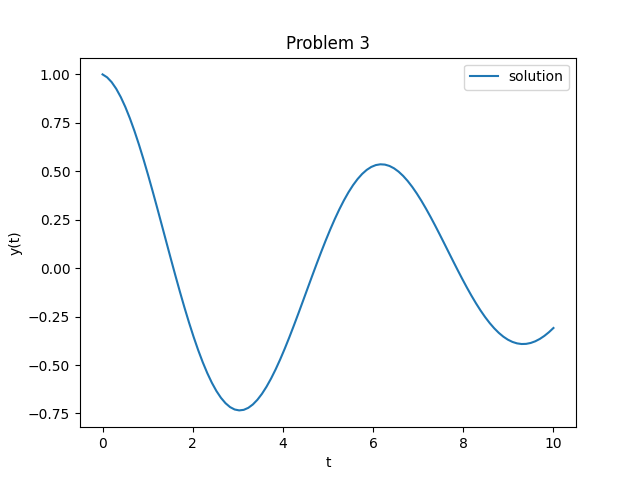
\includegraphics[width=0.7\linewidth]{./figures/solution_problem3}
\caption{Solution to the third ODE problem.}
\label{fig:solution_problem3}
\end{figure}

\subsection{Absence of control of the continuous solution approximation for typical IVODE solvers}
\label{section:end_of_step_innacurate}
In this section, we discuss how conventional solvers employed in popular packages like the Scipy library solve IVODE problems. These libraries will often have the option of using an error control solver based on a Runge-Kutta pair which works as follows. The pair comes with a low order method and a high order method and will solve an ODE by taking a sequence of steps. The solver will take each step with both methods and use the difference between the higher order method and the lower order method to generate an error estimate for the discrete numerical solution at the end of the step. If the error estimate is within the user provided tolerance, the solver will accept the step and proceed to the next step. If the error estimate is not within the tolerance, the solver will reduce the step-size and attempt to take the step again. As the error of Runge-Kutta methods depends on the step-size, a smaller step-size will produce a smaller error. The solver will keep reducing the step-size until the user tolerance is satisfied and will then proceed to the next step. In an attempt to improve the efficiency, solvers will also increase the step-size when the estimated error is significantly smaller than the tolerance.

An issue with this approach is that the error estimate is computed only for the discrete numerical solution computed at the end of a step and thus the error control is only applied at the end of the step. An interpolant that provides a continuous solution approximation across the entire step is typically constructed by the solver and it is hoped that the error of the interpolant at points within the step is within the user-provided tolerance. However, as we will show below, this is sometimes not the case.

For this interpolant to provide a solution within the user provided tolerance, the theoritical interpolation error must be less than or equal to the error of the data being fitted. Thus we would ideally use an interpolant of at least order $O(h^{p})$ if the discrete solution is of order $O(h^{p})$. However, for high order methods, it becomes too expensive to construct an interpolant of the appropriate order. IVODE solvers will thus usually compromise and employ a lower order interpolant, that is less costly, but deliver less accuracy. 

Therefore, we are not guaranteed that the continuous approximate solution is error-controlled and not guaranteed that the interpolation error will not affect the continuous solution approximation. Figures $\ref{fig:no_middle_step_error_control_p2_dop853}$ and $\ref{fig:no_middle_step_error_control_p3_rk45}$ show some results obtained when Runge-Kutta solvers are applied to some of the test problems introduced in the previous section. In these figures, we plot the global error of the numerical solution, this is the difference between the exact solution and the computed solution over the time domain. The solvers apply error control to the discrete numerical solution at the end of the step but no error control of any type to the continuous numerical solution across the step.

\begin{figure}[H]
\centering
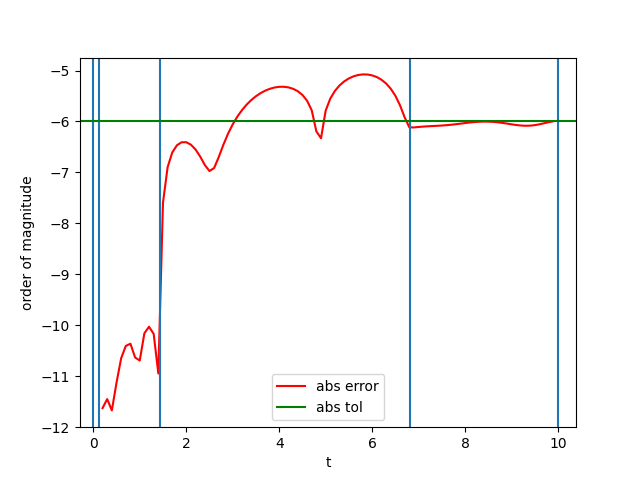
\includegraphics[width=0.7\linewidth]{./figures/no_middle_step_error_control_p2_dop853}
\caption{The Python `DOP853' solver on problem 2 with an absolute tolerance of $10^{-6}$ and a relative tolerance of $10^{-6}$. Steps are represented by the vertical lines.}
\label{fig:no_middle_step_error_control_p2_dop853}
\end{figure}

\begin{figure}[H]
\centering
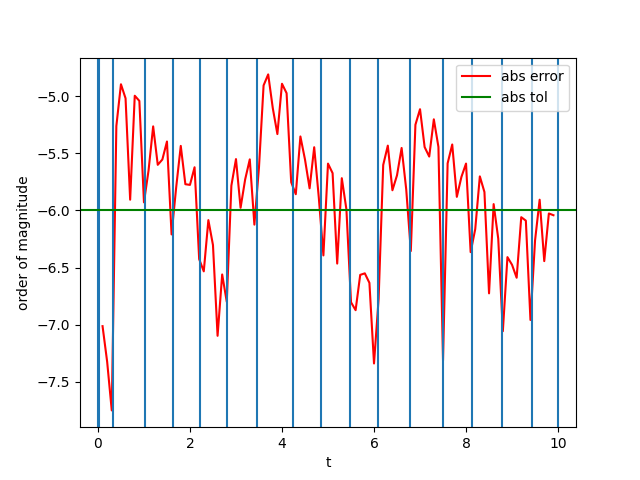
\includegraphics[width=0.7\linewidth]{./figures/no_middle_step_error_control_p3_rk45}
\caption{The Python `RK45' solver on problem 3 with an absolute tolerance of $10^{-6}$ and a relative tolerance of $10^{-6}$. Steps are represented by the vertical lines.}
\label{fig:no_middle_step_error_control_p3_rk45}
\end{figure}

Figure $\ref{fig:no_middle_step_error_control_p2_dop853}$ and $\ref{fig:no_middle_step_error_control_p3_rk45}$ shows the errors in the middle of each step obtained when applying `DOP853' to problem 2 and `RK45' to problem 3 with an absolute tolerance of $10^{-6}$ and a relative tolerance of $10^{-6}$. We can see that the solution values at the end of each step typically satisfy the tolerance. However we can clearly see that the solution values (obtained from the built-in interpolant constructed by the solver) at points within each steps, have errors up to one order of magnitude larger than the tolerance. 

We note that when a user asks for a solution whose estimated error is within a tolerance of $10^{-i}$, they expect the solution to have an estimated error that is within that tolerance for the whole time domain. However, the decision to not satisfy the user provided tolerance throughout the step is made in the interest of efficiency and the loss of accuracy in the middle of the step is the tradeoff. The goal of modern IVODE solvers is to provide a continuous solution approximation across the whole time domain. The user's expectation is that the solution approximations across each step also satisfies the tolerance as ODE solvers can be integral part of larger software packages where their approximate solutions are differentiated, integrated and manipulated in ways such that a sufficiently accurate continuous approximate solution is required. 

In this chapter, we attempt to provide an efficient way of constructing interpolants that can then be used to control the defect of the continuous approximate solution across the step and thus throughout the whole time domain.

\subsection{Defect control and the cost of traditional Continuous Runge-Kutta methods}
\label{section:crk_related_work}
In this section we introduce the `defect' of a continuous approximate solution of an ODE and explain how the control of that defect provides a type of error control of the continuous numerical solution.

In the context of numerical ODEs, the defect, denoted by $\delta(t)$,  is the amount by which the continuous numerical solution, $u(t)$, fails to satisfy the ODE. When the ODE is $y'(t) = f(t, y(t))$, the defect is 

\begin{equation}
\delta(t) = |u'(t) - f(t, u(t))|.
\end{equation}

Calculating the defect requires that the continuous approximate solution computed by the solver to also be differentiable. The idea of defect control is relatively new as differentiable solutions to ODEs can be expensive to calculate. Several investigations in this direction are outlined in \cites{MR2600928}{MR1950917}{MR1803189}{MR1239829}{MR997658}{MR996053}. In this work, the defect control method employs a continuous RK method for which the number of stages grows exponentially with the order of the method as shown in Table $\ref{tab:crk_nstages}$. In this chapter, we will compute a defect controlled continuous solution with no additional cost. A typical Runge-Kutta solver will thus be able to employ the usual number of stages required for the discrete Runge-Kutta method and still produce an accurate continuous solution.

\begin{table}[h]
\caption {Number of stages for discrete vs continuous RK method.} 
\label{tab:crk_nstages}
\begin{center}
\begin{tabular}{ c c c c} 
order   & discrete & continuous & asymptotically correct defect \\ 
4 & 4  & 4   & 8 \\ 
5 & 5  & 6   & 12 \\ 
6 & 6  & 7   & 15 \\ 
7 & 7  & 9   & 20 \\ 
8 & 8  & 13  & 27 \\ 
\end{tabular}
\end{center}
\end{table}

Though the defect is defined for the whole step, the estimation of the maximum defect within a step is what is important. If the maximum defect is within the tolerance, then the defect of the whole solution within the given step is within the tolerance. The key task is to find the location of the maximum defect within the step. One approach would be to sample the defect at several points and use the maximum value sampled. The problem with this approach is that each sampling of the defect requires an additional function evaluation. Thus we should not do too many samples. Work in this direction (cited above) involves constructing special interpolants that guarantee that (asymptotically) the maximum defect is at the same location within every step for every problem. This way only one function evaluation is required to sample the defect to obtain an estimate of the maximum defect. This is referred to as asymptotically correct defect control.

In the approach outlined in this chapter, we have observed experimentally that the maximum defect will tend to appear at one of two locations within the step. Thus in our approach, only two defect samplings must be done to get the maximum defect. Though we make an additional function evaluation compared to the asymptotically correct defect control, using no function evaluations to construct the interpolant guarantees that our method is more efficient especially for higher orders.


\subsection{Overview of our approach}
\label{section:basic_runge_kutta}
In this chapter, we will discuss simple IVODE solvers based on discrete Runge-Kutta methods of order 4, 6 and 8 and show that we can provide accurate continuous interpolant to augment the discrete solution computed by these RK methods without having to compute any additional function evaluations. In this section, we give an outline of the approach.

The first Runge-Kutta method upon which we build a prototype defect control solver is the classical $4^{th}$ order method that uses 4 stages; the second method is a Verner $6^{th}$ order method, taken from his 6(5) pair \cite{JimVernerRepo} that uses 9 stages, and the last method is a Verner $8^{th}$ order method from an 8(7) pair that uses 13 stages \cite{MR1239829}. 

The solvers that we have written use a simple step selection strategy. If the estimated maximum defect is greater than $tol$, the solver rejects the step and attempts to retake it again with half the step-size. If the estimated maximum defect is less than $0.1tol$, the solver accepts the step and doubles the step-size for the next step. We will elaborate on the initial step-size used by each solver later in the chapter.

We now note that the solver is not optimised. A more thorough analysis of how the solver behaves and thus a more refined step selection algorithm will produce a better solver in practice. The software we consider in this chapter only serves as a proof of concept for a more elaborate solver. 

\section{Multistep interpolants for zero-cost defect control for a Runge Kutta method}
\label{section:equipping_rk4_with_HBs}
In this section we will consider a multistep interpolant approach, built on the classical $4^{th}$ order Runge Kutta method (RK4), that allows for defect control. We will augment the discrete Runge-Kutta solution with interpolants of $4^{th}$, $6^{th}$ and $8^{th}$ orders respectively and explain the challenges and the efficiency and accuracy of each interpolant. 

We first note that Runge-Kutta methods are very convenient in that they are one step methods. At any point, when taking the next step, the method does not have to take into consideration the size of the previous steps and this is convenient as the solver can choose the size of the next step in the most optimal way based only on how the error estimate compares with the tolerance for the current step. 

The first interpolant that we discuss is a single step interpolant. It is the classical Hermite cubic of order 4. We will show how this interpolant can be used to perform defect control and discuss the limitations of this interpolant. 

We then show how a Hermite-Birkhoff interpolant of $6^{th}$ order can address the issues that we identified for the $4^{th}$ order interpolant. We will give an overview of how a $6^{th}$ order interpolant is derived and show the results of applying defect control using this interpolant to solve the three test problems. 

We will then use a similar approach to derive an $8^{th}$ order Hermite-Birkhoff interpolant and show why the approach used for the $6^{th}$ order interpolant needs to be modified for the $8^{th}$ order. We then discuss another approach to derive an $8^{th}$ order interpolant that addresses the issue with the previous one and show the results of using this $8^{th}$ order interpolant as the basis for computing defect controlled numerical solutions of the three test problems.


\subsection{The Classical $4^{th}$ order RK method with a $4^{th}$ order Hermite Cubic Interpolant}
The Hermite cubic spline is a very widely used interpolant. The basic idea is that we can use the derivative values and not just the solution values to get more data to fit an interpolant. Given points $(t_i, y_i)$ and $(t_{i + 1}, y_{i + 1})$ with derivatives $f_i$ and $f_{i + 1}$ (here $f_i = f(t_i, y_i)$ and $f_{i+1}=f(t_{i+1}, y_{i+1})$), respectively, the interpolant across the step $[t_i, t_{i + 1}]$ of size $h_i$ is defined as:

\begin{equation}
\label{eqn:HB4}
u(t_i + \theta h) = h_{00}(\theta)y_i +  h_ih_{10}(\theta)f_i + h_{01}(\theta)y_{i + 1} + h_ih_{11}(\theta)f_{i + 1}, 
\end{equation}
and its derivative is:
\begin{equation}
u'(t_i + \theta h) = h_{00}'(\theta)y_i/h_i +  h_{10}'(\theta)f_i + h_{01}'(\theta)y_{i + 1}/h_i + h_{11}'(\theta)f_{i + 1}. 
\end{equation}

The quantity $\theta$ is:
\begin{equation}
\label{eqn:HB4_theta}
\theta = (t - t_i) / h_i.
\end{equation}

The functions $h_{00}(\theta)$, $h_{01}(\theta)$, $h_{10}(\theta)$ and $h_{11}(\theta)$ are each cubics defined such that $u(t_i)= y_i$, $u'(t_i) = f_i$, $u(t_{i+1}) = y_{i + 1}$ and $u'(t_{i + 1}) = f_{i + 1}$. When $\theta$ is 0, $t_i + \theta h_i$ is $t_i$ and thus only $h_{00}(0)$ should be 1 and all the others cubic should evaluate to 0. Also only $h_{10}'(0)$ should be 1 and the derivatives of all the other cubics should evaluate to 0. When $\theta$ is 1, $t_i + \theta h_i$ is $t_{i + 1}$ and thus only $h_{01}(1)$ should be 1 and all the other cubics should evaluate to 0. Also only $h_{11}'(1)$ should be 1 and the derivatives of all the other cubics should be 0.

We will assume that each of the cubics has the form $a\theta^3 + b\theta^2 + c\theta + d$, where $a, b, c$ and $d$ are coefficients to be determined, and note that for each cubic we know its value for $\theta$ at 0 and 1 and the values of its derivatives for $\theta$ at 0 and 1. We thus have 4 equations for each cubic. Thus we can solve the system for each cubic to get the values of a, b, c and d for each cubic.

We now note that from equations $\ref{eqn:HB4}$ and $\ref{eqn:HB4_theta}$, we can evaluate both the interpolant and its derivative for any $\theta$ in $[t_i, t_{i + 1}]$ and therefore we can form $\delta(t + \theta h_i) = u'(t_i + \theta h_i) - f(t_i + \theta h_i, u(t_i + \theta h_i))$ which can be used to sample the defect for any $\theta$.

We will show below experimentally that the maximum defect occurs consistently approximately either at $x_i + 0.2h_i$ or at $x_i + 0.8h_i$ so that we just need to sample the defect twice in order to obtain an estimate of the maximum defect on the step.

We now note that the interpolant comes at no additional cost. We only need $(x_i, y_i, f_i)$ and $(x_{i + 1}, y_{i + 1}, f_{i + 1})$ to be stored as the discrete solution approximation are computed by the RK method. No additional stages or function evaluations are required for the construction of the interpolant itself. 

For the remainder of this chapter, we will refer to the Hermite cubic interpolant as `HB4'.

\paragraph{Problem 1 results}
Figures $\ref{fig:rk4_with_hb4_p1_global_defect}$, $\ref{fig:rk4_with_hb4_p1_global_error}$ and $\ref{fig:rk4_with_hb4_p1_scaled_defects}$ shows the results of using RK4 with HB4 on Problem 1. We note that an absolute tolerance of $10^{-6}$ is applied on the maximum defect estimate within the step and this can be observed to occur at $0.2h$ and $0.8h$ for a step of size h. See Figure $\ref{fig:rk4_with_hb4_p1_scaled_defects}$, to see the scaled defect reaching a maximum near these points. (The figure shows the shape of the defect for each of the steps that were taken to solve Problem 1 using RK4 with HB4. All the defects were scaled vertically to be in the range [0, 1] and scaled horizontally so that they map onto [0, 1]. We see that over all steps and problems, the defect has two clear peaks at $0.2h$ and $0.8h$.) We note that we are able to successfully control the defect of the continuous numerical solution using this approach; see Figure $\ref{fig:rk4_with_hb4_p1_global_defect}$. To obtain these results, we sampled the defect at many points within each step.

\begin{figure}[H]
\centering
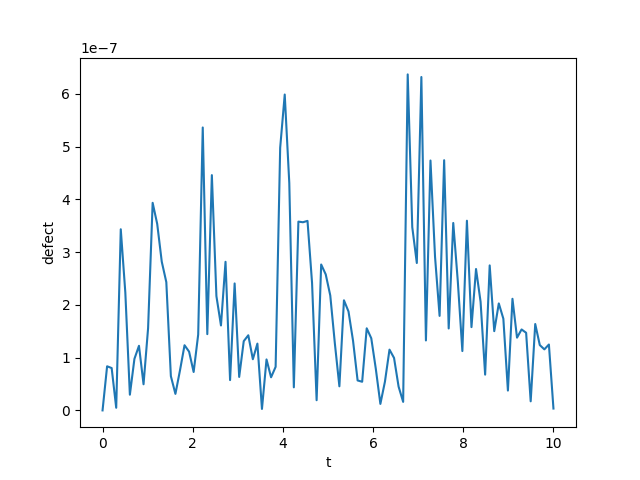
\includegraphics[width=0.7\linewidth]{./figures/rk4_with_hb4_p1_global_defect}
\caption{Defect across the entire domain for RK4 with HB4 on problem 1 at an absolute tolerance of $10^{-6}$.}
\label{fig:rk4_with_hb4_p1_global_defect}
\end{figure}

\begin{figure}[H]
\centering
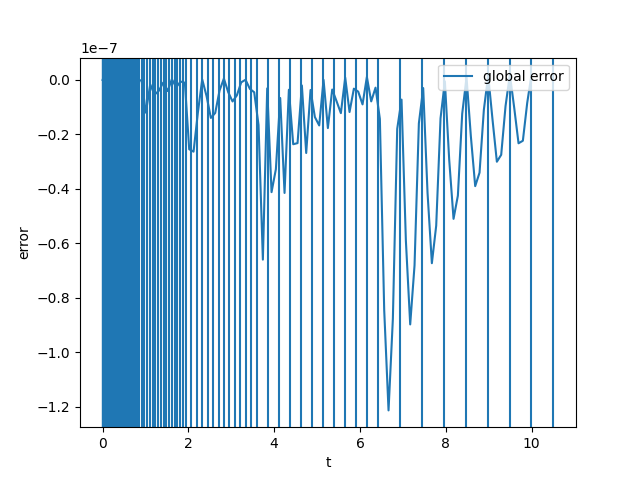
\includegraphics[width=0.7\linewidth]{./figures/rk4_with_hb4_p1_global_error}
\caption{Global Error for RK4 with HB4 on problem 1 at an absolute tolerance of $10^{-6}$.}
\label{fig:rk4_with_hb4_p1_global_error}
\end{figure}

\begin{figure}[H]
\centering
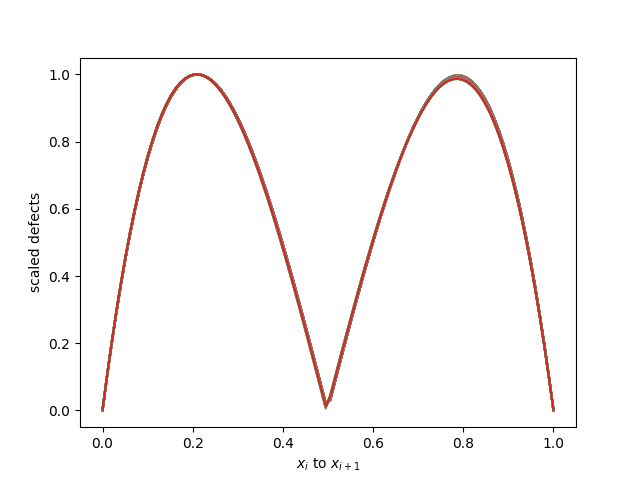
\includegraphics[width=0.7\linewidth]{./figures/rk4_with_hb4_p1_scaled_defects}
\caption{Scaled defects over all steps for RK4 with HB4 on problem 1 at an absolute tolerance of $10^{-6}$ mapped onto $[0, 1]$. The defect has the same shape on every step.}
\label{fig:rk4_with_hb4_p1_scaled_defects}
\end{figure}

\paragraph{Problem 2 results}
Figures $\ref{fig:rk4_with_hb4_p2_global_defect}$, $\ref{fig:rk4_with_hb4_p2_global_error}$ and $\ref{fig:rk4_with_hb4_p2_scaled_defects}$ shows the results of using RK4 with HB4 on Problem 2. We note that an absolute tolerance of $10^{-6}$ is applied on the maximum defect estimate within the step and this can be observed to occur at $0.2h$ and $0.8h$ for a step of size, h. See Figure $\ref{fig:rk4_with_hb4_p2_scaled_defects}$, to see the scaled defect reaching a maximum near these points. We note that we are able to successfully control the defect of the continuous numerical solution using this approach; see Figure $\ref{fig:rk4_with_hb4_p2_global_defect}$. For Problem 2, the defect is noisy on small steps and we do not get two clean peaks. However, we note that we quite consistently get the maximum defects at $0.2h$ and $0.8h$ and thus we only require two defect samplings.

\begin{figure}[H]
\centering
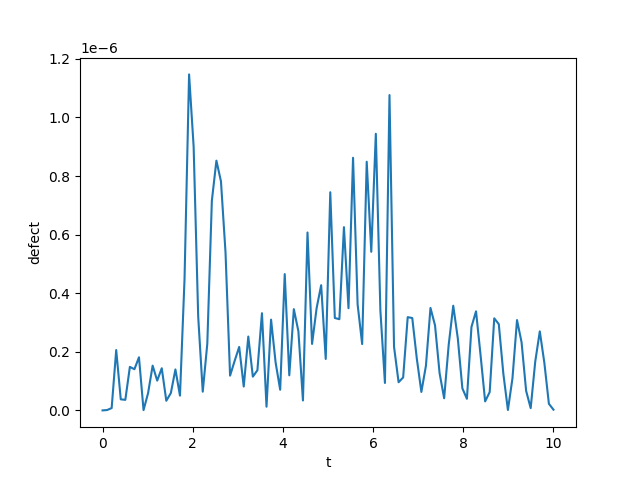
\includegraphics[width=0.7\linewidth]{./figures/rk4_with_hb4_p2_global_defect}
\caption{Defect across the entire domain for RK4 with HB4 on problem 2 at an absolute tolerance of $10^{-6}$.}
\label{fig:rk4_with_hb4_p2_global_defect}
\end{figure}

\begin{figure}[H]
\centering
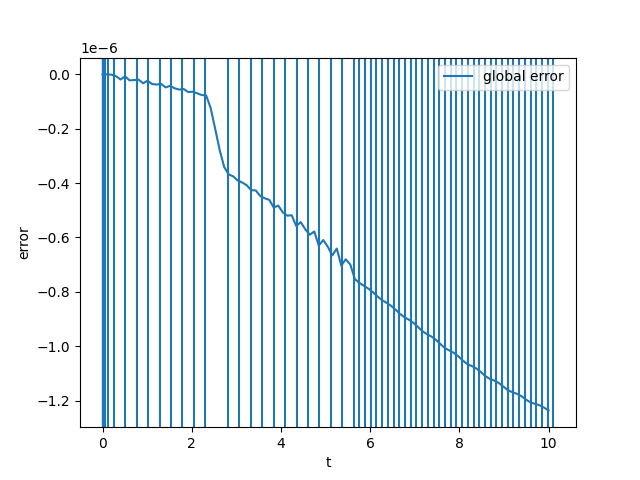
\includegraphics[width=0.7\linewidth]{./figures/rk4_with_hb4_p2_global_error}
\caption{Global Error for RK4 with HB4 on problem 2 at an absolute tolerance of $10^{-6}$. There is more variation in the shape of the defect for this problem but the maximum defect occurs near either $0.2h$ or $0.8h$.}
\label{fig:rk4_with_hb4_p2_global_error}
\end{figure}

\begin{figure}[H]
\centering
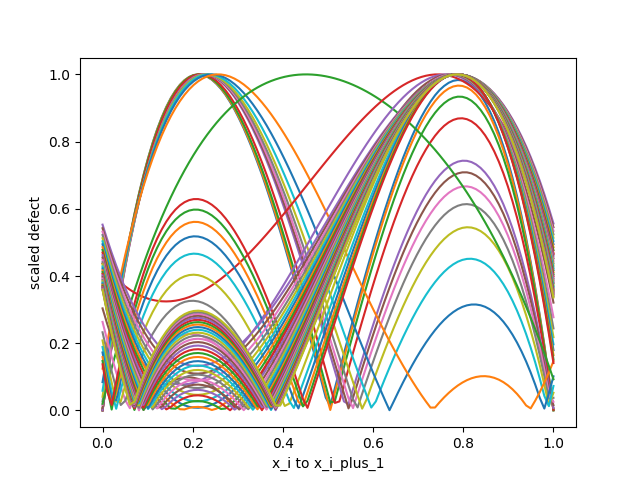
\includegraphics[width=0.7\linewidth]{./figures/rk4_with_hb4_p2_scaled_defects}
\caption{Scaled defects over all steps taken for RK4 with HB4 on problem 2 at an absolute tolerance of $10^{-6}$ mapped onto $[0, 1]$. There is more variation in the shape of the defect for this problem but the maximum defect occurs near either $0.2h$ or $0.8h$. }
\label{fig:rk4_with_hb4_p2_scaled_defects}
\end{figure}

\begin{figure}[H]
\centering
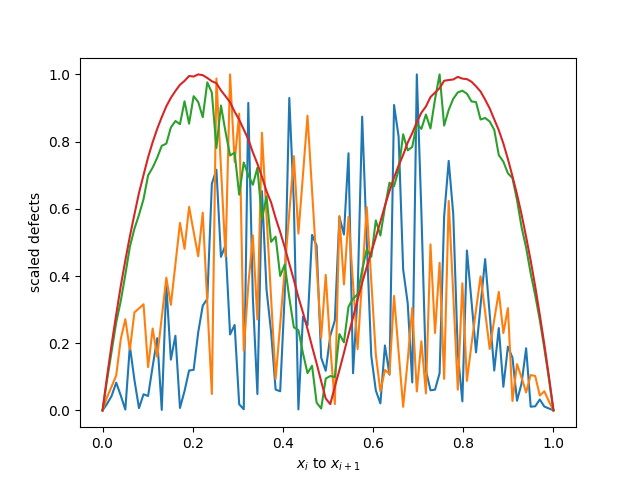
\includegraphics[width=0.7\linewidth]{./figures/rk4_with_hb4_p2_scaled_defects_small_steps}
\caption{Scaled defects small steps taken RK4 with HB4 on problem 2 at an absolute tolerance of $10^{-6}$ mapped onto $[0, 1]$.}
\label{fig:rk4_with_hb4_p2_scaled_defects_small_steps}
\end{figure}

\paragraph{Problem 3 results}
Figures $\ref{fig:rk4_with_hb4_p3_global_defect}$, $\ref{fig:rk4_with_hb4_p3_global_error}$ and $\ref{fig:rk4_with_hb4_p3_scaled_defects}$ shows the results of using RK4 with HB4 on Problem 3. We note that an absolute tolerance of $10^{-6}$ is applied on the maximum defect within the step and this can be shown to occur at $0.2h$ and $0.4h$ along a step of size, h. See Figure $\ref{fig:rk4_with_hb4_p3_scaled_defects}$, to see the scaled defect reaching a maximum near these points. We note that we are able to successfully control the defect of the continuous numerical solution using this approach, see Figure $\ref{fig:rk4_with_hb4_p3_global_defect}$. 

\begin{figure}[H]
\centering
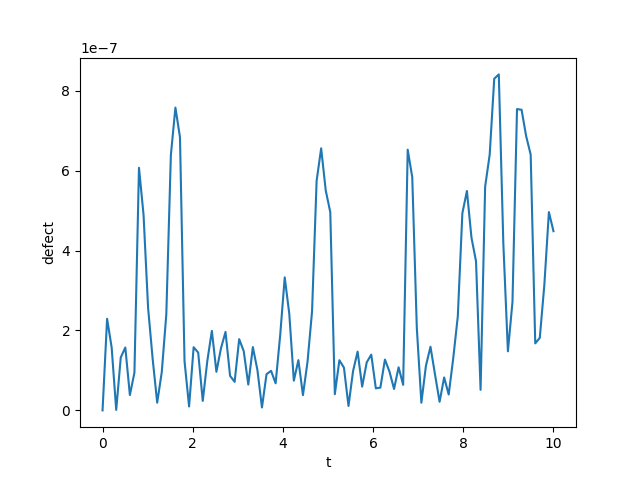
\includegraphics[width=0.7\linewidth]{./figures/rk4_with_hb4_p3_global_defect}
\caption{Defect across the entire domain for RK4 with HB4 on problem 3 at an absolute tolerance of $10^{-6}$.}
\label{fig:rk4_with_hb4_p3_global_defect}
\end{figure}

\begin{figure}[H]
\centering
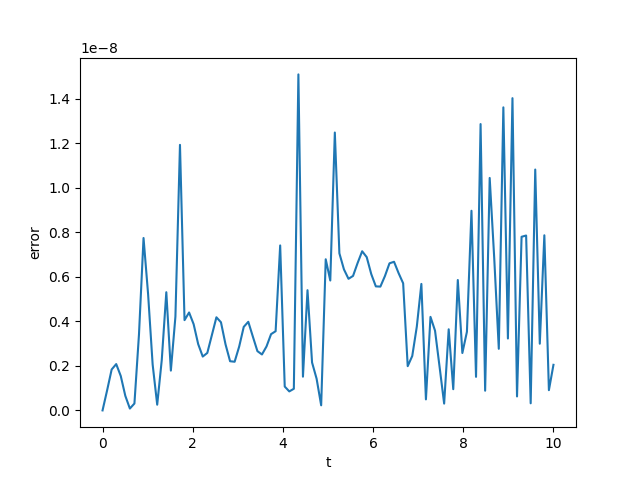
\includegraphics[width=0.7\linewidth]{./figures/rk4_with_hb4_p3_global_error}
\caption{Global Error of RK4 with HB4 for problem 3 at an absolute tolerance of $10^{-6}$.}
\label{fig:rk4_with_hb4_p3_global_error}
\end{figure}

\begin{figure}[H]
\centering
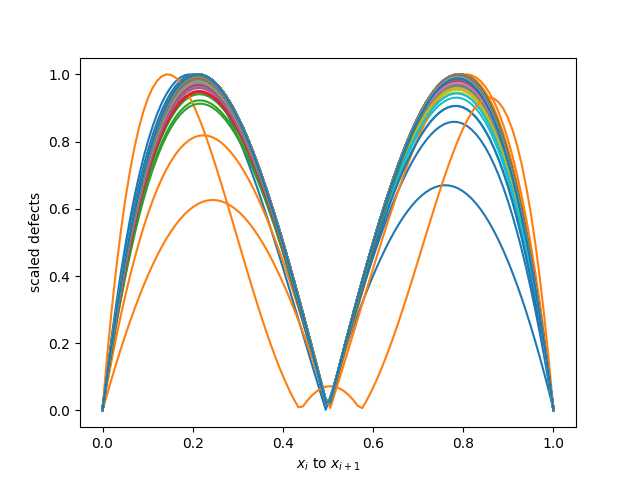
\includegraphics[width=0.7\linewidth]{./figures/rk4_with_hb4_p3_scaled_defects}
\caption{Scaled defects over all steps taken for RK4 with HB4 on problem 3 at an absolute tolerance of $10^{-6}$ mapped onto $[0, 1]$. The shape of the defect stays relatively similar but there are two peaks, one at $0.2h$ and another at $0.8h$.}
\label{fig:rk4_with_hb4_p3_scaled_defects}
\end{figure}

\paragraph{Efficiency data and discussion of the interpolation error}
We now present the number of steps that were taken by the solver to solve each problem along with the number of successful steps.

\begin{table}[h]
\caption {Number of steps taken by RK4 using defect control with HB4.} \label{tab:rk4_with_hb4_nsteps}
\begin{center}
\begin{tabular}{ c c c } 
Problem & successful steps & total steps \\ 
1       & 88                         & 88 \\ 
2       & 59                         & 62 \\
3       & 225                        & 232 \\
\end{tabular}
\end{center}
\end{table}

The Hermite cubic, HB4, is an interpolant of $4^{th}$ order. However, to perform defect control we need to calculate the derivative of this interpolant. Since we are differentiating the interpolant, the order of the derivative is 3. The numerical solution is of order 4 as we are using RK4 and thus the derivative of the interpolant is less accurate than the ODE solution. We need a way to get an interpolant whose derivative is at least of order 4 so that the error of the derivative of the interpolant is not larger than the error of the discrete numerical solution obtained from the RK4 method.

To do that, in the next section, we will introduce a new interpolation scheme based on a Hermite-Birkhoff interpolant which is of $6^{th}$ order and will thus have a derivative of order 5.

\subsection{RK4 with a $6^{th}$ order Hermite-Birkhoff interpolant}
We first start by noting that this interpolant is a multistep interpolant as it depends on the previous step.

Suppose that the step taken by a solver to go from $t_i$ to $t_{i + 1}$ is of size $h$. We can define the size of the step from $t_{i - 1}$ to $t_i$ by using a weight $\alpha$ such that the size of the step from $t_{i - 1}$ to $t_i$ is $\alpha$h. Then given the solution values and the derivative values at all the three points, i.e, $(t_{i-1}, y_{i - 1}, f_{i - 1})$, $(t_i, y_i, f_i)$ and $(t_{i + 1}, y_{i + 1}, f_{i + 1})$, we can fit a two-step quintic interpolant of order 6 defined as such:
\begin{equation}
\begin{split}
u(t_i + \theta h) = d_{0}(\theta) y_{i-1} +  h_id_{1}(\theta)f_{i-1} \\
+ d_{2}(\theta)y_i     +  h_id_{3}(\theta)f_i
+ d_{4}(\theta)y_{i + 1} + h_id_{5}(\theta)f_{i + 1}, \\
\end{split}
\end{equation}
and its derivative is
\begin{equation}
\begin{split}
u'(t_i + \theta h) = d_{0}'(\theta)y_{i-1}/h_i +  d_{1}'(\theta)f_{i-1} \\
+ d_{2}'(\theta)y_i/h_i     +  d_{3}'(\theta)f_i
+ d_{4}'(\theta)y_{i + 1}/h_i + d_{5}'(\theta)f_{i + 1}. \\
\end{split}
\end{equation}
As before, $\theta$ is:
\begin{equation}
\theta = (t - t_i) / h_i.
\end{equation}

This time $\theta$ is allowed to vary between -$\alpha$ and 1 such that $t_i + \theta$h is $t_{i - 1}$ when $\theta$ is $-\alpha$, $t_i$ when $\theta$ is 0 and $t_{i + 1}$ when $\theta$ is 1.

Each of $d_0(\theta)$, $d_1(\theta)$, $d_2(\theta)$, $d_3(\theta)$, $d_4(\theta)$, and $d_5(\theta)$ is a quintic of the form $a\theta^5 + b\theta^4 + c\theta^3 + d\theta^2 + e\theta + f$ where the six coefficients for each can be found by solving a linear system of 6 equations in terms of $\alpha$. The six equations are obtained as follows. First, for $\theta = -\alpha$, only $d_0(\theta)$ evaluates to 1 and all the other quintic polynomials evaluate to 0 as $u(t_i - \alpha h) = u(t_{i - 1}) = y_{i - 1}$. Also at this $\theta$, only the derivative of $d_1(\theta)$ evaluates to 1 and all the other quintic polynomials' derivatives evaluate to 0 as $u'(t_i - \alpha h) = u'(t_{i - 1}) = f_{i - 1}$. When $\theta$ is 0, only $d_2(\theta)$ evaluates to 1 and all the other polynomials evaluate to 0 as $u(t_i - 0(h)) = u(t_i) = y_i$. Also at this $\theta$ value, only the derivative of $d_3(\theta)$ evaluates to 1 and all the other quintic polynomial derivatives evaluate to 0 as $u'(t_i - 0(h)) = u'(t_i) = f_i$. When $\theta$ is 1, only $d_4(\theta)$ evaluates to 1 and all the other polynomials evaluate to 0 as $u(t_i + 1(h)) = u(t_{i+1}) = y_{i+1}$. Also at this $\theta$, only the derivative of $d_5(\theta)$ evaluates to 1 and all the other quintic polynomial derivatives evaluate to 0 as $u'(t_i - 1(h)) = u'(t_{i+1}) = f_{i+1}$. With these six conditions, we can get six equations for each quintic in terms of $\alpha$ and, using a symbolic management package, we can solve all of these to find the six quintic polynomials. (Their coefficients will be given in terms of $\alpha$.)

We again note that as the solver is stepping across the problem domain, these interpolants are constructed for no additional cost in terms of evaluation of $f(t, y(t))$. We just need to store $(t_{i-1}, y_{i - 1}, f_{i - 1})$, $(t_i, y_i, f_i)$ and $(t_{i + 1}, y_{i + 1}, f_{i + 1})$ as these quantities are being computed by the RK method. We will also observe that the defect peaks at two positions within the new step, $[t_i, t_{i+1}]$, and thus, we can find the maximum defect by only sampling the defect twice. This technique provides an efficient defect control of a continuous approximate solution.

The interpolant defined as above will be referred to as `HB6' for the remainder of this chapter. We note that it is of order 6 and its derivative is of order 5.

We now note that for RK4 as the solution values are only accurate to $4^{th}$ order. We want the derivative of the interpolant to be of order 4 or higher so that interpolation error is relatively negligible. This scheme satisfies this condition and we will see below how this allows us to take fewer time steps to solve a given problem than when HB4 was used with RK4.

\paragraph{Problem 1 results}
Figures $\ref{fig:rk4_with_hb6_p1_global_defect}$, $\ref{fig:rk4_with_hb6_p1_global_error}$ and $\ref{fig:rk4_with_hb6_p1_scaled_defects}$ shows the results of using RK4 with HB6 on Problem 1. We note that an absolute tolerance of $10^{-6}$ is applied on the maximum defect within the step and this can be shown to occur at $0.3h$ and $0.8h$ along a step of size, h. See Figure $\ref{fig:rk4_with_hb6_p1_scaled_defects}$, to see the scaled defect reaching a maximum near these points. We note that we are able to successfully control the defect of the continuous numerical solution using this approach; see Figure $\ref{fig:rk4_with_hb6_p1_global_defect}$. 

\begin{figure}[H]
\centering
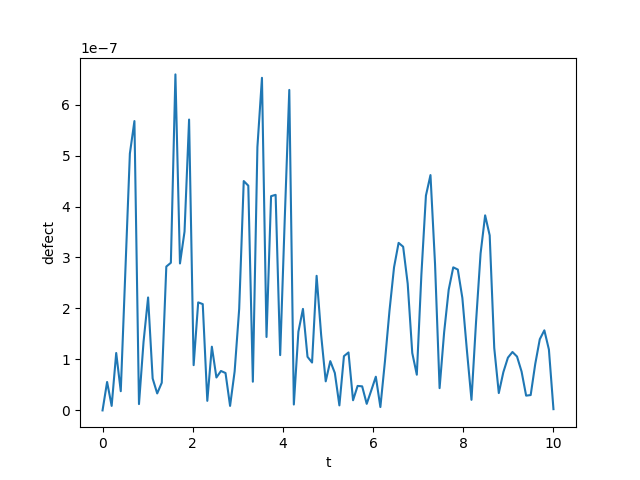
\includegraphics[width=0.7\linewidth]{./figures/rk4_with_hb6_p1_global_defect}
\caption{Defect across the entire domain for RK4 with HB6 on problem 1 at an absolute tolerance of $10^{-6}$.}
\label{fig:rk4_with_hb6_p1_global_defect}
\end{figure}

\begin{figure}[H]
\centering
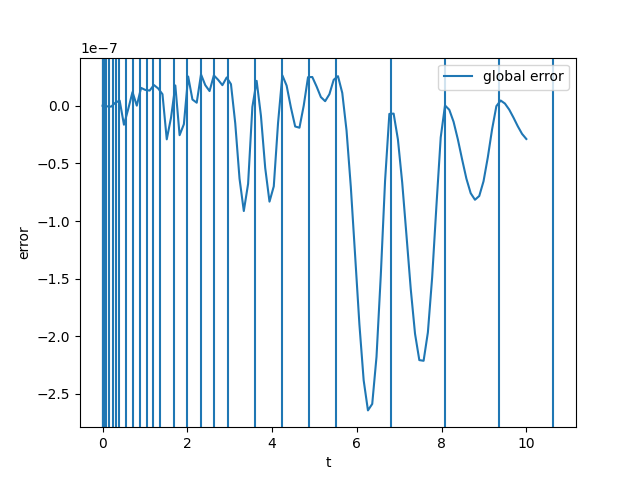
\includegraphics[width=0.7\linewidth]{./figures/rk4_with_hb6_p1_global_error}
\caption{Global Error for RK4 with HB6 on problem 1 at an absolute tolerance of $10^{-6}$.}
\label{fig:rk4_with_hb6_p1_global_error}
\end{figure}

\begin{figure}[H]
\centering
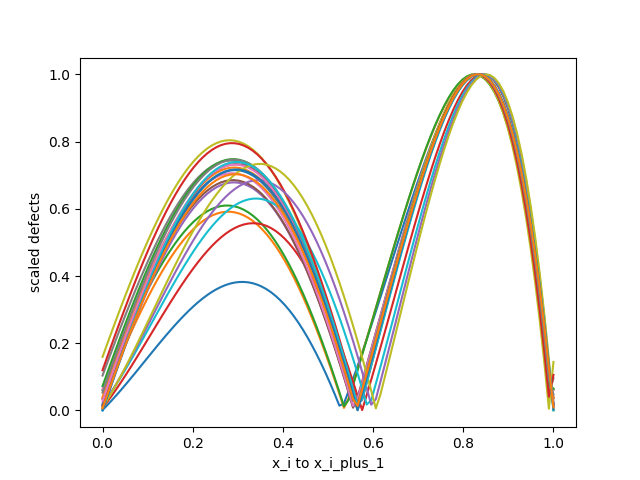
\includegraphics[width=0.7\linewidth]{./figures/rk4_with_hb6_p1_scaled_defects}
\caption{Scaled defects for RK4 with HB6 on problem 1 at an absolute tolerance of $10^{-6}$ mapped into $[0, 1]$.}
\label{fig:rk4_with_hb6_p1_scaled_defects}
\end{figure}

\paragraph{Problem 2 results}
Figures $\ref{fig:rk4_with_hb6_p2_global_defect}$, $\ref{fig:rk4_with_hb6_p2_global_error}$ and $\ref{fig:rk4_with_hb6_p2_scaled_defects}$ shows the results of using the modification of RK4 with HB6 on Problem 2. We note that an absolute tolerance of $10^{-6}$ is applied on the maximum defect within the step and this can be shown to occur at $0.8h$ along a step of size, h. See Figure $\ref{fig:rk4_with_hb6_p2_scaled_defects}$, to see the scaled defect reaching a maximum near these points. We note that we are able to successfully control the defect of the continuous numerical solution using this approach, see Figure $\ref{fig:rk4_with_hb6_p2_global_defect}$. For Problem 2, the defect is noisy on small steps and we do not get two clean peaks. However, we note that we quite consistently get the maximum defects at $0.4h$ and $0.8h$ and thus we only require two samplings.

\begin{figure}[H]
\centering
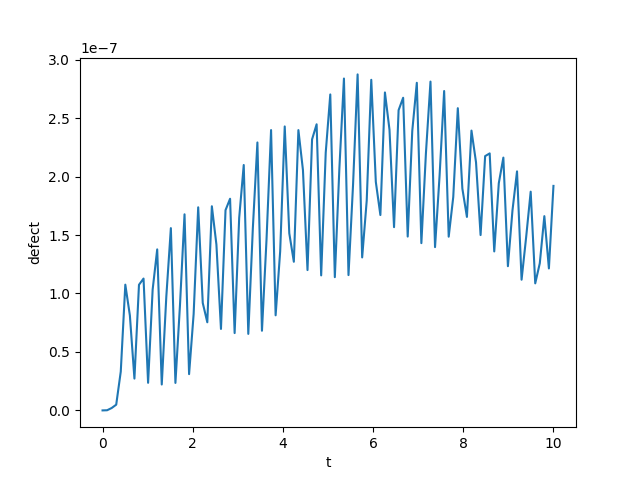
\includegraphics[width=0.7\linewidth]{./figures/rk4_with_hb6_p2_global_defect}
\caption{Defect across the entire domain for RK4 with HB6 on problem 2 at an absolute tolerance of $10^{-6}$.}
\label{fig:rk4_with_hb6_p2_global_defect}
\end{figure}

\begin{figure}[H]
\centering
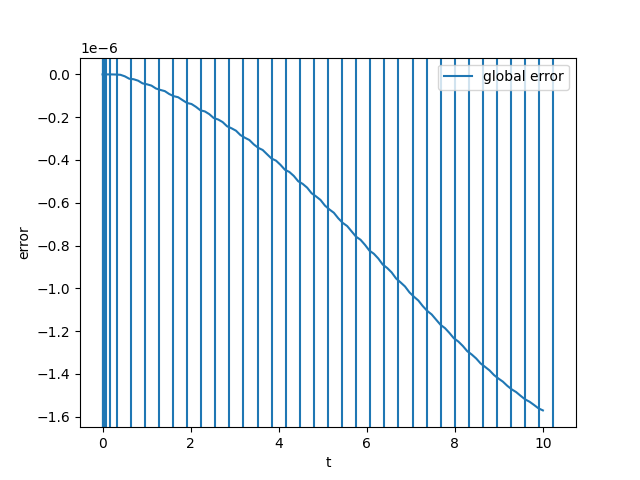
\includegraphics[width=0.7\linewidth]{./figures/rk4_with_hb6_p2_global_error}
\caption{Global Error for RK4 with HB6 on problem 2 at an absolute tolerance of $10^{-6}$.}
\label{fig:rk4_with_hb6_p2_global_error}
\end{figure}

\begin{figure}[H]
\centering
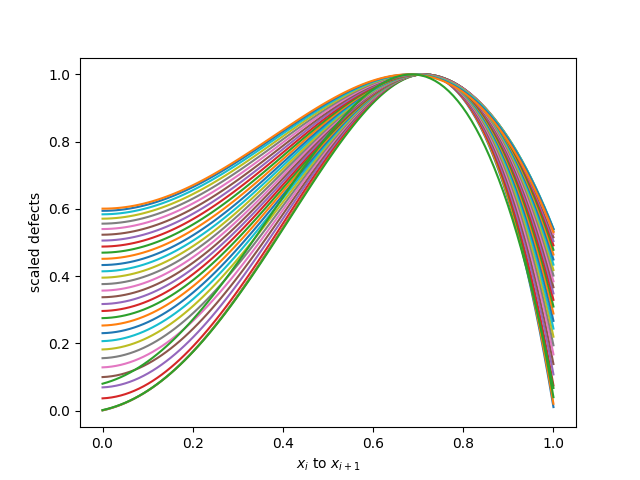
\includegraphics[width=0.7\linewidth]{./figures/rk4_with_hb6_p2_scaled_defects}
\caption{Scaled defects for RK4 with HB6 on problem 2 at an absolute tolerance of $10^{-6}$ mapped into $[0, 1]$.}
\label{fig:rk4_with_hb6_p2_scaled_defects}
\end{figure}

\begin{figure}[H]
\centering
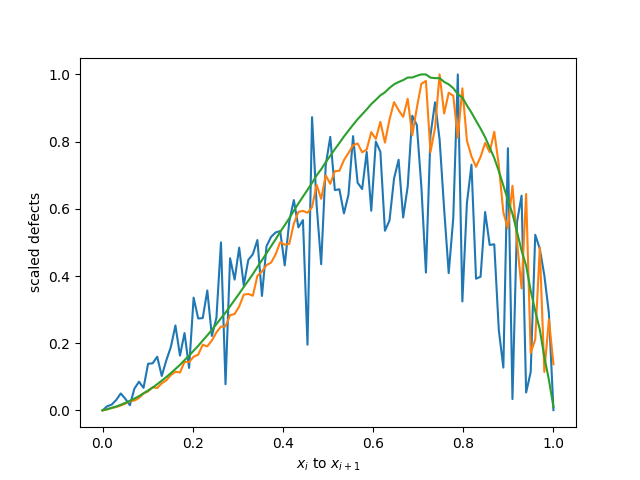
\includegraphics[width=0.7\linewidth]{./figures/rk4_with_hb6_p2_scaled_defects_small_steps}
\caption{Scaled defects for RK4 with HB6 on small steps on problem 2 at an absolute tolerance of $10^{-6}$ mapped into $[0, 1]$. Despite the noise, the maximum defect occurs near $0.8h$.}
\label{fig:rk4_with_hb6_p2_scaled_defects_small_steps}
\end{figure}

\paragraph{Problem 3 results}
Figures $\ref{fig:rk4_with_hb6_p3_global_defect}$, $\ref{fig:rk4_with_hb6_p3_global_error}$ and $\ref{fig:rk4_with_hb6_p3_scaled_defects}$ shows the results of using RK4 with HB6 on Problem 3. We note that an absolute tolerance of $10^{-6}$ is applied on the maximum defect within the step and this can be shown to occur at $0.8h$ along a step of size, h. See Figure $\ref{fig:rk4_with_hb6_p3_scaled_defects}$, to see the scaled defect reaching a maximum near these points. We note that we are able to successfully control the defect of the continuous numerical solution using this approach, see Figure $\ref{fig:rk4_with_hb6_p3_global_defect}$. 


\begin{figure}[H]
\centering
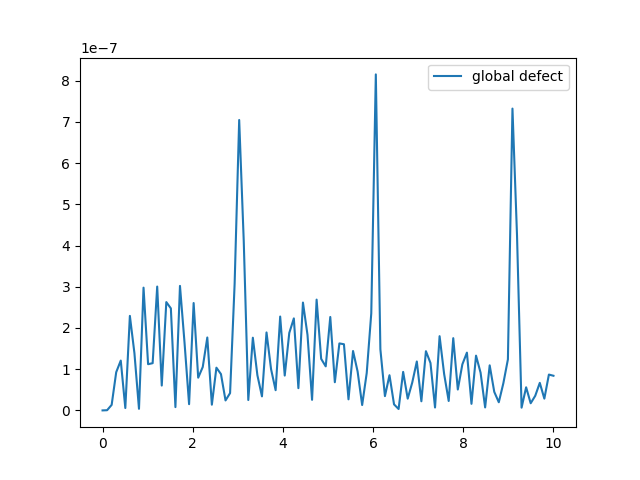
\includegraphics[width=0.7\linewidth]{./figures/rk4_with_hb6_p3_global_defect}
\caption{Defect across the entire domain for RK4 with HB6 on problem 3 at an absolute tolerance of $10^{-6}$.}
\label{fig:rk4_with_hb6_p3_global_defect}
\end{figure}

\begin{figure}[H]
\centering
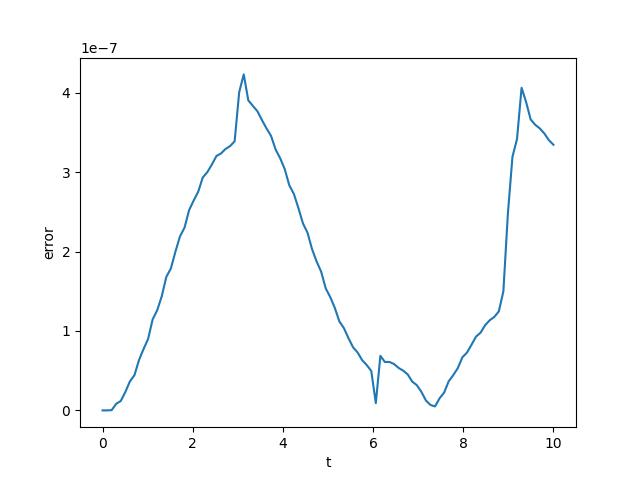
\includegraphics[width=0.7\linewidth]{./figures/rk4_with_hb6_p3_global_error}
\caption{Global Error for RK4 with HB6 on problem 3 at an absolute tolerance of $10^{-6}$.}
\label{fig:rk4_with_hb6_p3_global_error}
\end{figure}

\begin{figure}[H]
\centering
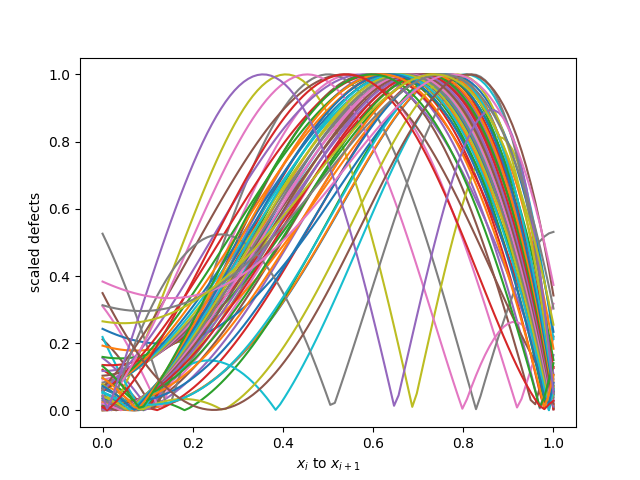
\includegraphics[width=0.7\linewidth]{./figures/rk4_with_hb6_p3_scaled_defects}
\caption{Scaled defects for RK4 with HB6 on problem 3 at an absolute tolerance of $10^{-6}$ mapped into $[0, 1]$.}
\label{fig:rk4_with_hb6_p3_scaled_defects}
\end{figure}

We note that the defects are not as clean they were in the case with HB4. There are two peaks most of the time at around $0.4h$ and $0.8h$ but as was the case in the third problem, the peak sometimes appears at $0.6h$. However, we can see that the defect is still being controlled. We will also see that it is twice as fast as it uses around half the number of steps as HB4.

\begin{table}[h]
\caption {Number of steps taken by RK4 when modified to do defect control with HB6 vs HB4.} \label{tab:rk4_with_hb6_nsteps}
\begin{center}
\begin{tabular}{ c c c c c } 
Problem & succ. steps HB4 & succ. steps HB6 & nsteps HB4  & nsteps HB6 \\ 
1       & 88                 &        27          & 88         & 27 \\ 
2       & 59                 &        36          & 62         & 40 \\
3       & 225                &        62          & 232        & 73 \\
\end{tabular}
\end{center}
\end{table}

Table $\ref{tab:rk4_with_hb6_nsteps}$ shows how the number of steps is less than half when we use HB6 as opposed to HB4. This is entirely because the error of the interpolant and its derivative are smaller than the error of the discrete solution values at the end of each step.

\paragraph{Issues with $\alpha$ values}
The issue with this scheme is that the interpolant is a multistep interpolant while the Runge-Kutta method is a one step method. The Hermite Birkhoff interpolant, HB6, is based on two steps and the parameter $\alpha$ defines how big the previous step is compared to the actual step. The error term in the Hermite-Birkhoff interpolant is minimised when the size of the two steps are the same size, i.e, when $\alpha$ is 1. The error term is proportional to $(t + \alpha)^2t^2(t - 1)^2$. When $\alpha$ differs from 1, the accuracy of the interpolant is reduced.

In Figure $\ref{fig:hb6_alpha_v_shape}$, we show the results of a simple experiment to illustrate how the accuracy of this scheme depends on the value of $\alpha$. We place 3 data points along the t-axis such that their distances apart are $\alpha$h and h for several values of $\alpha$ and we vary h from 1 to $10^{-7}$; we then report on the maximum defect for each h.

\begin{figure}[H]
\centering
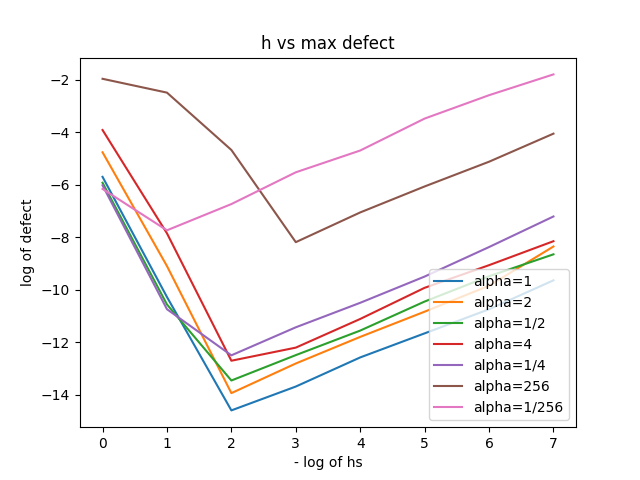
\includegraphics[width=0.7\linewidth]{./figures/hb6_alpha_v_shape}
\caption{HB6 maximum defect based on different values of $\alpha$.}
\label{fig:hb6_alpha_v_shape}
\end{figure}

Figure $\ref{fig:hb6_alpha_v_shape}$ shows that at $\alpha$ = 2, $\frac{1}{2}$, 4 and $\frac{1}{4}$, the defect are comparable to those that we get when $\alpha$ is at 1. However, we see that $\alpha = 256$ and $\frac{1}{256}$, the smallest defect that we can obtain for any $h$ value is much larger.

We note that in solving the 3 test problems, $\alpha$ is very rarely bigger than 4 or smaller than $\frac{1}{4}$ and thus, we can be satisfied with the approach that we have considered in this section. We discuss the situation further in Section $\ref{section:keeping_alpha_at_1}$. We note that in order for the results given in Figure $\ref{fig:hb6_alpha_v_shape}$ to be relevant, we would have to be considering a very sharp tolerance since for reasonable values of $\alpha$, e.g, $2$, $\frac{1}{2}$, $4$ and $\frac{1}{4}$, the interpolants all deliver very small defects of $10^{-12}$ to $10^{-14}$.

Another idea would be to use an even higher order interpolant so as to reduce the interpolation error more. We note that with with the approach we consider here, there is no additional cost to get the higher order interpolant. In the next section, we discuss an $8^{th}$ order interpolant and show how to derive such an interpolant.

\subsection{RK4 with an $8^{th}$ order Hermite-Birkhoff interpolant}
\label{section:HB8_derivation}
\paragraph{Derivation of HB8}
In this section, we discuss a derivation of an $8^{th}$ order interpolant. To derive an 8 order interpolant, we need 4 data points over 3 steps. We need the data values to be $(t_i, y_i, f_i)$, as well as the two previous steps $(t_{i-1}, y_{i-1}, f_{i-1})$ and $(t_{i-2}, y_{i-2}, f_{i-2})$, and the right hand end of the current step step, $(t_{i+1}, y_{i+1}, f_{i+1})$. We present two schemes: 
\begin{itemize}
\item The first scheme has the parameters $\alpha$ and $\beta$ are associated with the previous two steps, so the three steps are of the size $\beta h$, $\alpha h$ and $h$ respectively. Thus the scheme establishes the base step-size to be that of the third step. 

\item The second scheme has the parameter $\alpha$ associated with the rightmost step and the parameter $\beta$ associated with the previous step; the middle step is the base step. Thus the sizes for the steps are $\alpha h$, $h$ and $\beta h$. 

\end{itemize}


\paragraph{First HB8 Scheme}
In the first scheme, the step sizes are $\beta h$, $\alpha h$ and $h$ respectively. The interpolant defined on $(t_{i-2}, y_{i-2}, f_{i-2})$, $(t_{i-1}, y_{i-1}, f_{i-1})$, $(t_i, y_i, f_i)$ and $(t_{i + 1}, y_{i + 1}, f_{i + 1})$ is defined as such:

\begin{equation}
\begin{split}
u(t_i + \theta h) = d_{0}(\theta)y_{i-2} +  h_id_{1}(\theta)f_{i-2} 
+ d_{2}(\theta)y_{i-1}     +  h_id_{3}(\theta)f_{i-1} \\
+ d_{4}(\theta)y_i     +  h_id_{5}(\theta)f_i 
+ d_{6}(\theta)y_{i + 1} + h_id_{7}(\theta)f_{i + 1}, \\
\end{split}
\end{equation}
and the derivative is:
\begin{equation}
\begin{split}
u'(t_i + \theta h) = d_{0}'(\theta)y_{i-2}/h_i +  d_{1}'(\theta)f_{i-2} 
+ d_{2}'(\theta)y_{i-1}/h_i   +  d_{3}'(\theta)f_{i-1} \\
+ d_{4}'(\theta)y_i/h_i       +  d_{5}'(\theta)f_i 
+ d_{6}'(\theta)y_{i + 1}/h_i +  d_{7}'(\theta)f_{i + 1}. \\
\end{split}
\end{equation}
Again $\theta$ is:
\begin{equation}
\theta = (t - t_i) / h_i.
\end{equation}

This time $\theta$ is allowed to vary between $-\alpha-\beta$ and 1 such that $t_i + \theta$h is $t_{i-2}$ when $\theta$ is $-\alpha-\beta$, $t_{i-1}$ when $\theta$ is $-\alpha$, $t_i$ when $\theta$ is 0 and $t_{i + 1}$ when $\theta$ is 1. Also $d_0(\theta)$, $d_1(\theta)$, $d_2(\theta)$, $d_3(\theta)$, $d_4(\theta)$, $d_5(\theta)$, $d_6(\theta)$ and $d_7(\theta)$ are all septic polynomials that will each have 8 coefficients.

Each septic polynomial is assumed to have the form $a\theta^7 + b\theta^6 + c\theta^5 + d\theta^4 + e\theta^3 + f\theta^2 + g\theta + h$ where the eight coefficients for each can be found in terms of $\alpha$ and $\beta$ by solving a linear system of 8 equations in terms of $\alpha$ and $\beta$. First at $\theta = -\alpha-\beta$, only $d_0(\theta)$ evaluates to 1 and all the other septic polynomials evaluate to 0 as $u(t_i - (\alpha+\beta) h) = u(t_{i - 2}) = y_{i - 2}$. Also at this $\theta$ value, only the derivative of $d_1(\theta)$ evaluates to 1 and all the other septic polynomial derivatives evaluate to 0 as $u'(t_i - (\alpha+\beta) h) = u'(t_{i - 2}) = f_{i - 2}$. When $\theta = -\alpha$, only $d_2(\theta)$ evaluates to 1 and all the other septic polynomials evaluate to 0 as $u(t_i - \alpha h) = u(t_{i - 1}) = y_{i - 1}$. Also at this $\theta$ value, only the derivative of $d_3(\theta)$ evaluates to 1 and all the other septic polynomial derivatives evaluate to 0 as $u'(t_i - \alpha h) = u'(t_{i - 1}) = f_{i - 1}$. When $\theta$ is 0, only $d_4(\theta)$ evaluates to 1 and all the other polynomials evaluate to 0 as $u(t_i - 0(h)) = u(t_i) = y_i$. Also at this $\theta$ value, only the derivative of $d_5(\theta)$ evaluates to 1 and all the other septic polynomial derivatives evaluate to 0 as $u'(t_i - 0(h)) = u'(t_i) = f_i$. When $\theta$ is 1, only $d_6(\theta)$ evaluates to 1 and all the other polynomials evaluate to 0 as $u(t_i + 1(h)) = u(t_{i+1}) = y_{i+1}$. Also at this $\theta$ value, only the derivative of $d_7(\theta)$ evaluates to 1 and all the other septic polynomial derivatives evaluate to 0 as $u'(t_i - 1(h)) = u'(t_{i+1}) = f_{i+1}$. With these eight conditions, we can get eight equations for each polynomial in terms of $\alpha$ and $\beta$ and, using a symbolic management package, we can solve all of these to find the eight septic polynomials.

We again note that as the solver is stepping through the problem, these interpolants can be obtained without the need for any extra evaluations of $f$. We just need to store the 4 data points $(t_{i-1}, y_{i - 1}, f_{i - 1})$, $(t_{i-1}, y_{i - 1}, f_{i - 1})$, $(t_i, y_i, f_i)$ and $(t_{i + 1}, y_{i + 1}, f_{i + 1})$.

The interpolant defined as above will be referred to as `HB8 First Scheme' for the remainder of this chapter. We note that it is of order 8 and its derivative is of order 7.

Unfortunately, this scheme has a serious issue. The accuracy of the interpolant is very sensitive to a slight change in $\alpha$ and/or $\beta$. This is because the error term is now proportional to $(t + \alpha + \beta)^2(t+\alpha)^2(t)^2(t-1)^2$. We note that the first term depends on both $\alpha$ and $\beta$ and thus very small deviations of these values from 1 will result in reduced accuracy. 

In Figure $\ref{fig:hb8_first_scheme_alpha_beta_test}$, we present the results of a simple experiment to illustrate this issue. We place 4 data points along the t-axis such that their distances apart are $\beta h$, $\alpha h$ and $h$ for several values of $\alpha$ and $\beta$ and we vary h from 1 to $10^{-10}$; we then report on the order of the maximum defect at each h for these values.

\begin{figure}[H]
\centering
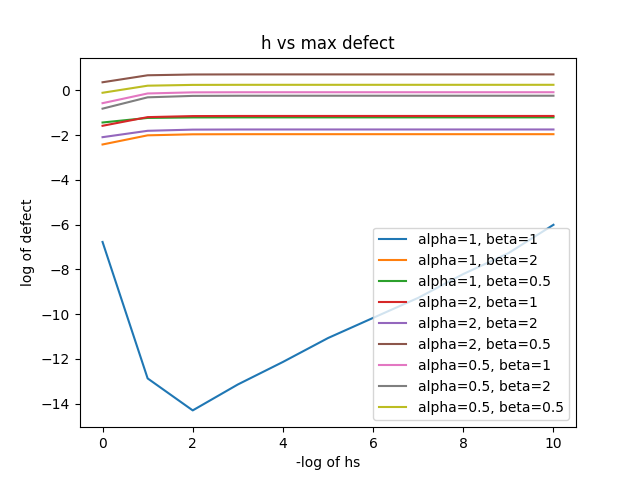
\includegraphics[width=0.7\linewidth]{./figures/hb8_first_scheme_alpha_beta_test}
\caption{HB8 First Scheme - maximum size of the defect based on different values of $\alpha$ and $\beta$.}
\label{fig:hb8_first_scheme_alpha_beta_test}
\end{figure}

From Figure $\ref{fig:hb8_first_scheme_alpha_beta_test}$, we can see the issue with this scheme. It only works if both $\alpha$ and $\beta$ are 1 and even small deviations from 1 for either $\alpha$ or $\beta$ drastically reduces the accuracy. More importantly, we can never halve the step with this method as if either $\alpha$ or $\beta$ is 2, the interpolant is not accurate to even one order of magnitude. We will now consider a second scheme which is more stable with respect to changes in $\alpha$ and $\beta$.

\paragraph{Second HB8 Scheme}
In this second scheme, we still use a 3 step interpolant with 4 data points $(t_{i-1}, y_{i-1}, f_{i-1})$, $(t_{i-2}, y_{i-2}, f_{i-2})$, $(t_{i}, y_{i}, f_{i})$ and $(t_{i+1}, y_{i+1}, f_{i+1})$ but now the distance between the points are $\alpha h$, $h$ and then $\beta h$. The middle step is the base step. This way the error term is approximately proportional to $(t- (1+\alpha))^2(t-1)^2t^2(t+\beta)^2$. We avoid the $(t-(\alpha+\beta))^2$ factor. We will show that this scheme is more resilient to changes in $\alpha$ and $\beta$.

Its derivation is very similar to the first scheme. The equation for the interpolant is:
\begin{equation}
\begin{split}
u(t_i + \theta h) = d_{0}(\theta)y_{i-2} +  h_id_{1}(\theta)f_{i-2} 
+ d_{2}(\theta)y_{i-1}     +  h_id_{3}(\theta)f_{i-1} \\
+ d_{4}(\theta)y_i     +  h_id_{5}(\theta)f_i 
+ d_{6}(\theta)y_{i + 1} + h_id_{7}(\theta)f_{i + 1}, \\
\end{split}
\end{equation}
and its derivative is:
\begin{equation}
\begin{split}
u'(t_i + \theta h) = d_{0}'(\theta)y_{i-2}/h_i +  d_{1}'(\theta)f_{i-2}
+ d_{2}'(\theta)y_{i-1}/h_i   +  d_{3}'(\theta)f_{i-1} \\
+ d_{4}'(\theta)y_i/h_i       +  d_{5}'(\theta)f_i
+ d_{6}'(\theta)y_{i + 1}/h_i +  d_{7}'(\theta)f_{i + 1}. \\
\end{split}
\end{equation}
Again $\theta$ is:
\begin{equation}
\theta = (t - t_i) / h_i.
\end{equation}

This time $\theta$ is allowed to vary between $-1-\alpha$ and $\beta$ such that $t_i + \theta h$ is $t_{i-2}$ when $\theta$ is $-1-\alpha$, $t_{i-1}$ when $\theta$ is -1, $t_i$ when $\theta$ is 0 and $t_{i + 1}$ when $\theta$ is $\beta$. Also $d_0(\theta)$, $d_1(\theta)$, $d_2(\theta)$, $d_3(\theta)$, $d_4(\theta)$, $d_5(\theta)$, $d_6(\theta)$ and $d_7(\theta)$ are all septic polynomials and will each have 8 conditions from which we can build a system to find their coefficients in terms of $\alpha$ and $\beta$.

Each is a septic of the form $a\theta^7 + b\theta^6 + c\theta^5 + d\theta^4 + e\theta^3 + f\theta^2 + g\theta + h$ where the eight coefficients for each can be found in terms of $\alpha$ and $\beta$ by solving a linear system of 8 equations in terms of $\alpha$ and $\beta$. First at $\theta = -1-\alpha$, only $d_0(\theta)$ evaluates to 1 and all the other septic polynomials evaluate to 0 as $u(t_i - (1+\alpha) h) = u(t_{i - 2}) = y_{i - 2}$. Also at this $\theta$ value, only the derivative of $d_1(\theta)$ evaluates to 1 and all the other septic polynomial derivatives evaluate to 0 as $u'(t_i - (1+\alpha) h) = u'(t_{i - 2}) = f_{i - 2}$. When $\theta = -1$, only $d_2(\theta)$ evaluates to 1 and all the other septic polynomials evaluate to 0 as $u(t_i - 1(h)) = u(t_{i - 1}) = y_{i - 1}$. Also at this $\theta$ value, only the derivative of $d_3(\theta)$ evaluates to 1 and all the other septic polynomials' derivatives evaluate to 0 as $u'(t_i - 1(h)) = u'(t_{i - 1}) = f_{i - 1}$. When $\theta$ is 0, only $d_4(\theta)$ evaluates to 1 and all the other polynomials evaluate to 0 as $u(t_i - 0(h)) = u(t_i) = y_i$. Also at this $\theta$ value, only the derivative of $d_5(\theta)$ evaluates to 1 and all the other septic polynomials' derivatives evaluate to 0 as $u'(t_i - 0(h)) = u'(t_i) = f_i$. When $\theta$ is $\beta$, only $d_6(\theta)$ evaluates to 1 and all the other polynomials evaluate to 0 as $u(t_i + \beta h) = u(t_{i+1}) = y_{i+1}$. Also at this $\theta$ value, only the derivative of $d_7(\theta)$ evaluates to 1 and all the other septic polynomial derivatives evaluate to 0 as $u'(t_i - \beta h) = u'(t_{i+1}) = f_{i+1}$. With these eight conditions, we can get eight equations for each septic in terms of $\alpha$ and $\beta$ and using a symbolic management package, we can solve all of these to find the 8 coefficients for each septic polynomial.

We now perform a simple experiment to show that the resultant interpolant is more resilient to changes in $\alpha$ and $\beta$. We place 4 data points along the x-axis such that their distance apart are $\alpha h$, $h$ and $\beta h$ for several values of $\alpha$ and $\beta$ and we vary $h$ from 1 to $10^{-10}$, we then report on the maximum defect at each $h$ for these values.

\begin{figure}[H]
\centering
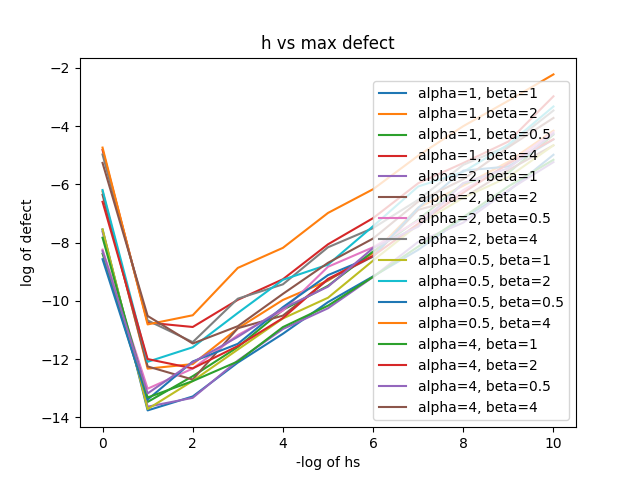
\includegraphics[width=0.7\linewidth]{./figures/hb8_second_scheme_alpha_beta_test}
\caption{HB8 Second Scheme - maximum order of accuracy based on different values of alpha and beta.}
\label{fig:hb8_second_scheme_alpha_beta_test}
\end{figure}

From Figure $\ref{fig:hb8_second_scheme_alpha_beta_test}$, we can see how this scheme is better than the first scheme. We can use $\alpha$ and $\beta$ equal to 2 and to 1/2 and still get a maximum defect of around $10^{-12}$ and we can even be accurate to $10^{-10}$ for both $\alpha$ and $\beta$ equal to 4 and $\frac{1}{4}$. 

For the remainder of this chapter, we will denote this $8^{th}$ order interpolant by HB8. Its derivative has order 7 and any subsequent higher derivative will have one less order.

\paragraph{Results}
We will now use RK4 with the second HB8 scheme and use the new defect control solver to solve the three test problems. We will show that we need to sample the defect only twice to estimate the maximum defect and that this scheme can provide good quality defect control.

\paragraph{Problem 1 results}
Figures $\ref{fig:rk4_with_hb8_p1_global_defect}$, $\ref{fig:rk4_with_hb8_p1_global_error}$ and $\ref{fig:rk4_with_hb8_p1_scaled_defects}$ shows the results of using RK4 with HB8 on Problem 1. We note that an absolute tolerance of $10^{-6}$ is applied on the maximum defect within the step and this can be shown to occur at $0.3h$ and $0.8h$ along a step of size, h. See Figure $\ref{fig:rk4_with_hb8_p1_scaled_defects}$, to see the scaled defect reaching a maximum near these points. We note that we are able to successfully control the defect of the continuous numerical solution using this approach, see Figure $\ref{fig:rk4_with_hb8_p1_global_defect}$. 

\begin{figure}[H]
\centering
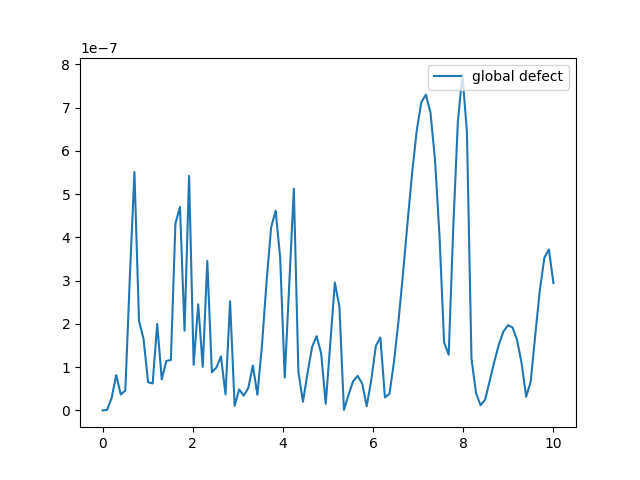
\includegraphics[width=0.7\linewidth]{./figures/rk4_with_hb8_p1_global_defect}
\caption{Defect across the entire domain for RK4 with HB8 on problem 1 at an absolute tolerance of $10^{-6}$.}
\label{fig:rk4_with_hb8_p1_global_defect}
\end{figure}

\begin{figure}[H]
\centering
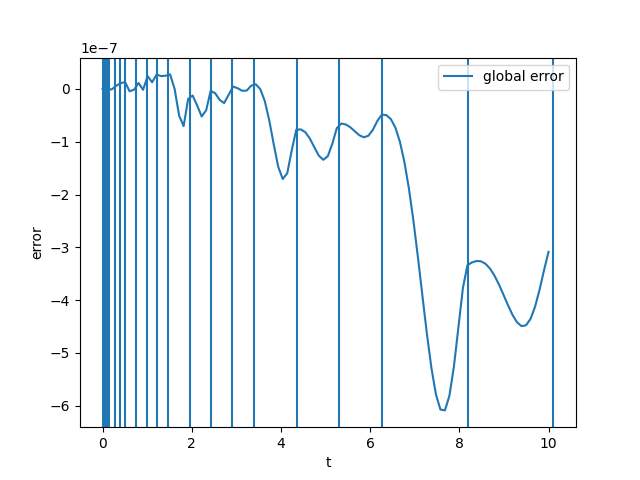
\includegraphics[width=0.7\linewidth]{./figures/rk4_with_hb8_p1_global_error}
\caption{Global Error for RK4 with HB8 on problem 1 at an absolute tolerance of $10^{-6}$.}
\label{fig:rk4_with_hb8_p1_global_error}
\end{figure}

\begin{figure}[H]
\centering
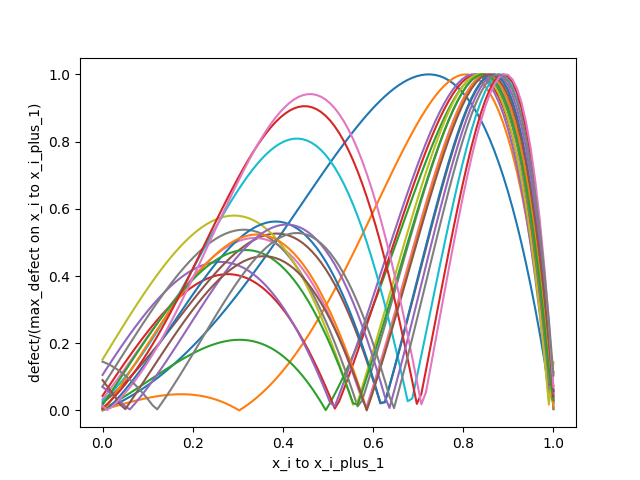
\includegraphics[width=0.7\linewidth]{./figures/rk4_with_hb8_p1_scaled_defects}
\caption{Scaled defects for RK4 with HB8 on problem 1 at an absolute tolerance of $10^{-6}$ mapped into $[0, 1]$.}
\label{fig:rk4_with_hb8_p1_scaled_defects}
\end{figure}

\paragraph{Problem 2 results}
Figures $\ref{fig:rk4_with_hb8_p2_global_defect}$, $\ref{fig:rk4_with_hb8_p2_global_error}$ and $\ref{fig:rk4_with_hb8_p2_scaled_defects}$ shows the results of using RK4 with HB8 on Problem 2. We note that an absolute tolerance of $10^{-6}$ is applied on the maximum defect within the step and this can be shown to occur at $0.8h$ along a step of size, h. See Figure $\ref{fig:rk4_with_hb8_p2_scaled_defects}$, to see the scaled defect reaching a maximum near these points. We note that we are able to successfully control the defect of the continuous numerical solution using this approach, see Figure $\ref{fig:rk4_with_hb8_p2_global_defect}$. 

\begin{figure}[H]
\centering
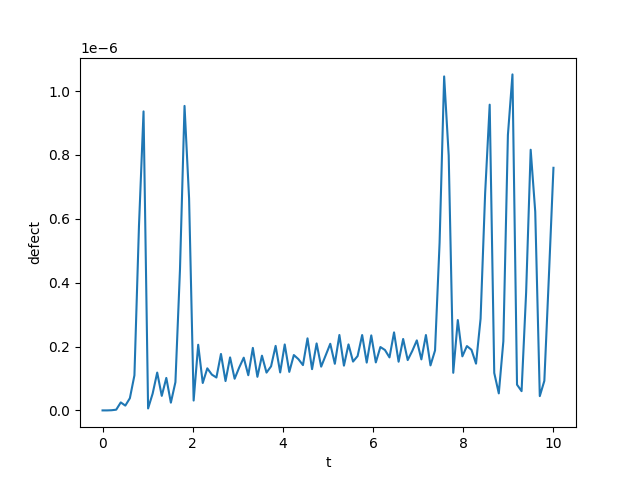
\includegraphics[width=0.7\linewidth]{./figures/rk4_with_hb8_p2_global_defect}
\caption{Defect across the entire domain for RK4 with HB8 on problem 2 at an absolute tolerance of $10^{-6}$.}
\label{fig:rk4_with_hb8_p2_global_defect}
\end{figure}

\begin{figure}[H]
\centering
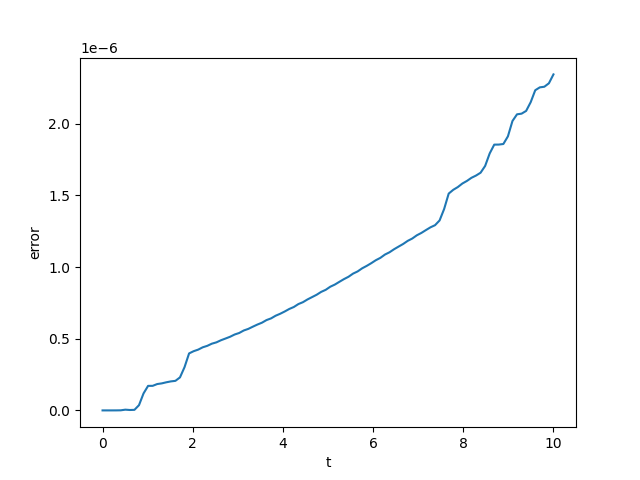
\includegraphics[width=0.7\linewidth]{./figures/rk4_with_hb8_p2_global_error}
\caption{Global Error for RK4 with HB8 on problem 2 at an absolute tolerance of $10^{-6}$.}
\label{fig:rk4_with_hb8_p2_global_error}
\end{figure}

\begin{figure}[H]
\centering
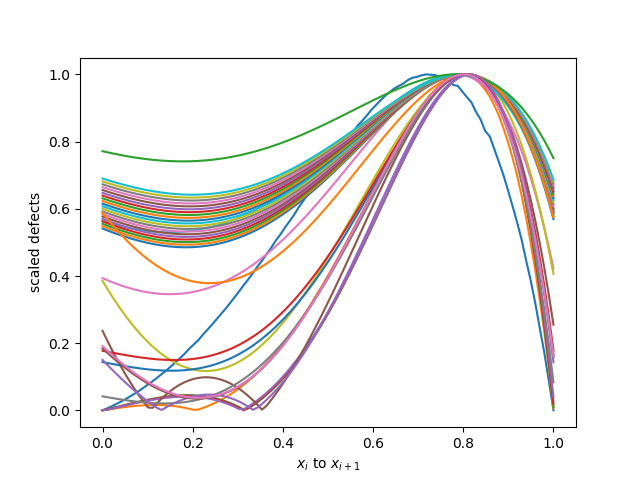
\includegraphics[width=0.7\linewidth]{./figures/rk4_with_hb8_p2_scaled_defects}
\caption{Scaled defects of RK4 with HB8 for problem 2 at an absolute tolerance of $10^{-6}$ mapped into $[0, 1]$.}
\label{fig:rk4_with_hb8_p2_scaled_defects}
\end{figure}

\paragraph{Problem 3 results}
Figures $\ref{fig:rk4_with_hb8_p3_global_defect}$, $\ref{fig:rk4_with_hb8_p3_global_error}$ and $\ref{fig:rk4_with_hb8_p3_scaled_defects}$ shows the results of using RK4 with HB8 on Problem 3. 
We note that an absolute tolerance of $10^{-6}$ is applied on the maximum defect within the step and this can be shown to occur at $0.3h$ or $0.8h$ along a step of size, h.  See Figure $\ref{fig:rk4_with_hb8_p3_scaled_defects}$, to see the scaled defect reaching a maximum near these points. We note that we are able to successfully control the defect of the continuous numerical solution using this approach, see Figure $\ref{fig:rk4_with_hb8_p3_global_defect}$. 

\begin{figure}[H]
\centering
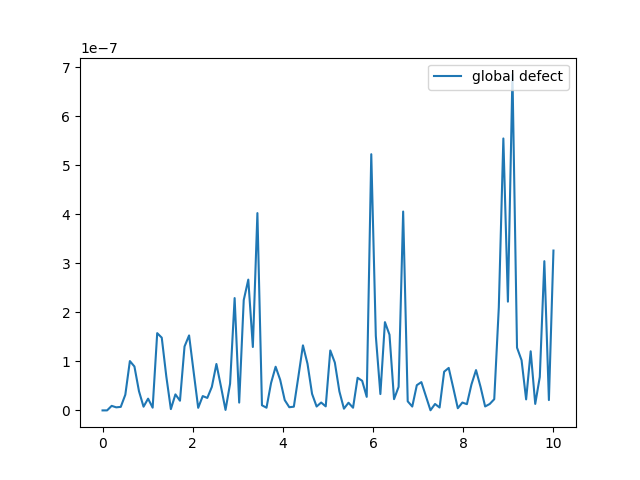
\includegraphics[width=0.7\linewidth]{./figures/rk4_with_hb8_p3_global_defect}
\caption{Defect across the entire domain of RK4 with HB8 on problem 3 at an absolute tolerance of $10^{-6}$.}
\label{fig:rk4_with_hb8_p3_global_defect}
\end{figure}

\begin{figure}[H]
\centering
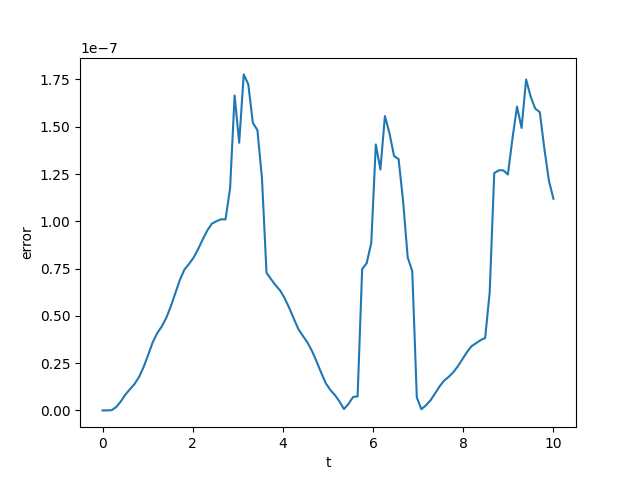
\includegraphics[width=0.7\linewidth]{./figures/rk4_with_hb8_p3_global_error}
\caption{Global Error of RK4 with HB8 on problem 3 at an absolute tolerance of $10^{-6}$.}
\label{fig:rk4_with_hb8_p3_global_error}
\end{figure}

\begin{figure}[H]
\centering
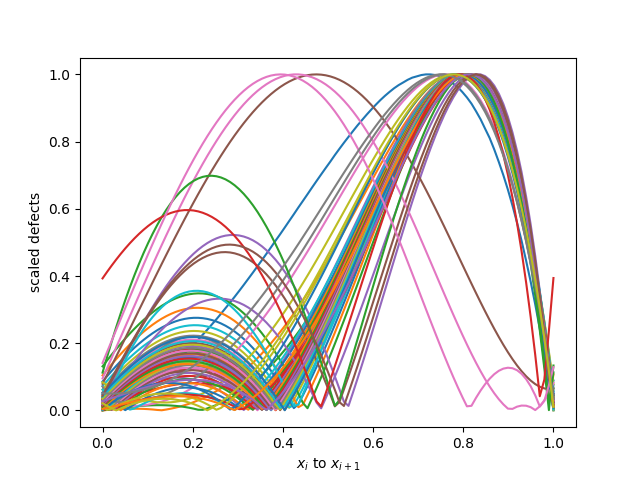
\includegraphics[width=0.7\linewidth]{./figures/rk4_with_hb8_p3_scaled_defects}
\caption{Scaled defects of RK4 with HB8 on problem 3 at an absolute tolerance of $10^{-6}$ mapped onto $[0, 1]$.}
\label{fig:rk4_with_hb8_p3_scaled_defects}
\end{figure}

We note that the defects are not as clean they were in the case with HB4. There are two peaks most of the time at around $0.3h$ and $0.8h$ but as was the case for the third problem in the previous tests, the peak sometimes appears at $0.6h$. However, we can see that the defect is still being controlled and thus that the error is still being controlled. We will also see that it is twice as fast as it uses around half the number of steps as HB4.

\begin{table}[h]
\caption {Number of steps taken by RK4 when modified to do defect control with HB8 vs when modified with HB6.} \label{tab:rk4_with_hb8_nsteps}
\begin{center}
\begin{tabular}{ c c c c c } 
Problem & succ. steps HB8 & succ. steps HB6 & nsteps HB8 & nsteps HB6 \\ 
1       & 20                 &        27          & 20         & 27\\ 
2       & 37                 &        36          & 60         & 40\\
3       & 69                 &        62          & 89         & 73\\
\end{tabular}
\end{center}
\end{table}

From Table $\ref{tab:rk4_with_hb8_nsteps}$, we can see that the number of steps with HB6 and with HB8 are relatively similar. This indicates that the interpolation error is no longer the limiting factor, even in HB6. The limiting factor is the discrete numerical solution which is as required. Thus though we can use RK4 with HB8 at the same cost as modifying RK4 with HB6, using HB8 does not improve the efficiency. Furthermore, HB8 is less stable to changes in $\alpha$ and $\beta$ than HB6 is to changes to $\alpha$. Thus RK4 is best augmented with HB6. However HB8 provides a new opportunity, we can now augment a $6^{th}$ order Runge Kutta method and possibly an $8^{th}$ order Runge-Kutta method, but in the latter case, the interpolation error will still affect the accuracy. Augmenting higher order methods with our HB6 and HB8 schemes is significant because as we have discussed in Section $\ref{section:crk_related_work}$ when using continuous Runge-Kutta solvers to obtain the interpolants, the number of stages grows exponentially with the order of the method. Our scheme is zero-cost and thus effective defect control using this approach will be relatively more efficient.


\subsection{RK4 with an $10^{th}$ order Hermite-Birkhoff interpolant}
\label{section:HB10_derivation}
\paragraph{Derivation of HB10 - the one that worked}


\paragraph{HB10 which by using HB8 in the middle}
We tried several HB10 scheme and the one that worked is created as follows. 
We extend HB8 second scheme by breaking its middle step and using the first half of the split middle step as the base step. So we break the step between $x_{i-1}$ and $x_i$ with an $x_{i - \frac{1}{2}}$. We then use the embedded HB8 that has been extended to calculate $y_{i- \frac{1}{2}}$ and make a function evaluation with these values to get $f_{i- \frac{1}{2}}$ to get 5 data points on which to build the interpolant.

The interpolant is thus defined over 4 steps of size $\alpha h$, $h$, $h$ and $\beta h$ over the data points $(x_{i-2}, y_{i-2}, f_{i-2})$, $(x_{i-1}, y_{i-1}, f_{i-1})$, $(x_{i-\frac{1}{2}}, y_{i-\frac{1}{2}}, f_{i-\frac{1}{2}})$, $(x_i, y_i, f_i)$ and $(x_{i + 1}, y_{i + 1}, f_{i + 1})$ is defined as such:

\begin{equation}
\begin{split}
u(t_{i-\frac{1}{2}} + \theta h) =
      d_0(\theta)y_{i-2}           + h_id_1(\theta)f_{i-2}\\
    + d_2(\theta)y_{i-1}           + h_id_3(\theta)f_{i-1}\\
    + d_4(\theta)y_{i-\frac{1}{2}} + h_id_5(\theta)f_{i-\frac{1}{2}}\\
    + d_6(\theta)y_i               + h_id_7(\theta)f_i \\
    + d_8(\theta)y_{i+1}           + h_id_9(\theta)f_{i+1}\\
\end{split}
\end{equation}
and the derivative is:
\begin{equation}
\begin{split}
u'(t_{i-\frac{1}{2}} + \theta h) = 
      d_0'(\theta)y_{i-2}/h_i           + d_1'(\theta)f_{i-2}\\
    + d_2'(\theta)y_{i-1}/h_i           + d_3'(\theta)f_{i-1}\\
    + d_4'(\theta)y_{i-\frac{1}{2}}/h_i + d_5'(\theta)f_{i-\frac{1}{2}}\\
    + d_6'(\theta)y_i/h_i               + d_7'(\theta)f_i \\
    + d_8'(\theta)y_{i+1}/h_i           + d_9'(\theta)f_{i+1}\\
\end{split}
\end{equation}
Again $\theta$ is:
\begin{equation}
\theta = (t - x_{i-\frac{1}{2}}) / h_i.
\end{equation}

The step between $x_{i-1}$ and $x_{i-\frac{1}{2}}$ is the base step with $\theta=0$ at $x_\frac{1}{2}$. This way the error terms have terms in $1 + \alpha$ and $1 + \beta$ instead of $2 + \alpha$ on one side and $\beta$ on another side. Not having $2 + \alpha$ reduces the error term. 

This time $\theta$ is allowed to vary between $-1-\alpha$ and $1+\beta$ such that $t_{i-\frac{1}{2}} + \theta$h is $t_{i-2}$ when $\theta$ is $-1-\alpha$, $t_{i-1}$ when $\theta$ is $-1$, $t_{i-\frac{1}{2}}$ at $\theta$ is 0, $t_i$ when $\theta$ is $1$ and $t_{i + 1}$ when $\theta$ is $1+\beta$. Also $d_0(\theta)$, $d_1(\theta)$, $d_2(\theta)$, $d_3(\theta)$, $d_4(\theta)$, $d_5(\theta)$, $d_6(\theta)$, $d_7(\theta)$, $d_8(\theta)$ and $d_9(\theta)$ are all nonic polynomials that will each have 10 coefficients.

Each nonic polynomial is assumed to have the form $a\theta^9 + b\theta^8 + c\theta^7 + d\theta^6 + e\theta^5 + f\theta^4 + g\theta^3 + h\theta^2 + i\theta + j$ where the 10 coefficients for each can be found in terms of $\alpha$ and $\beta$ by solving a linear system of 10 equations in terms of $\alpha$ and $\beta$. 


First at $\theta = -1-\alpha$, only $d_0(\theta)$ evaluates to 1 and all the other nonic polynomials evaluate to 0 as $u(t_{i-\frac{1}{2}} - (1+\alpha) h) = u(t_{i - 2}) = y_{i - 2}$.  Also at this $\theta$ value, only the derivative of $d_1(\theta)$ evaluates to 1 and all the other nonic polynomial derivatives evaluate to 0 as $u'(t_{i-\frac{1}{2}} - (1+\alpha) h) = u'(t_{i - 2}) = f_{i - 2}$. 

When $\theta = -1$, only $d_2(\theta)$ evaluates to 1 and all the other nonic polynomials evaluate to 0 as $u(t_{i-\frac{1}{2}} - h) = u(t_{i - 1}) = y_{i - 1}$. Also at this $\theta$ value, only the derivative of $d_3(\theta)$ evaluates to 1 and all the other nonic polynomial derivatives evaluate to 0 as $u'(t_{i-\frac{1}{2}} - h) = u'(t_{i - 1}) = f_{i - 1}$. 

When $\theta$ is 0, only $d_4(\theta)$ evaluates to 1 and all the other nonic polynomials evaluate to 0 as $u(t_{i-\frac{1}{2}} - 0(h)) = u(t_{i-\frac{1}{2}}) = y_{i-\frac{1}{2}}$. Also at this $\theta$ value, only the derivative of $d_5(\theta)$ evaluates to 1 and all the other nonic polynomial derivatives evaluate to 0 as $u'(t_{i-\frac{1}{2}} - 0(h)) = u'(t_{i-\frac{1}{2}}) = f_{i-\frac{1}{2}}$. 

When $\theta$ is 1, only $d_6(\theta)$ evaluates to 1 and all the other nonic polynomials evaluate to 0 as $u(t_{i-\frac{1}{2}} + 1(h)) = u(t_{i}) = y_{i}$. Also at this $\theta$ value, only the derivative of $d_7(\theta)$ evaluates to 1 and all the other nonic polynomial derivatives evaluate to 0 as $u'(t_{i-\frac{1}{2}} - 1(h)) = u'(t_{i}) = f_{i}$. 

When $\theta$ is $1 + \beta$, only $d_8(\theta)$ evaluates to 1 and all the other nonic polynomials evaluate to 0 as $u(t_{i-\frac{1}{2}} + (1 + \beta)(h)) = u(t_{i+1}) = y_{i+1}$. Also at this $\theta$ value, only the derivative of $d_9(\theta)$ evaluates to 1 and all the other nonic polynomial derivatives evaluate to 0 as $u'(t_{i-\frac{1}{2}} - (1 + \beta)(h)) = u'(t_{i+1}) = f_{i+1}$. 

With these 10 conditions, we can get 10 equations for each polynomial in terms of $\alpha$ and $\beta$ and, using a symbolic management package, we can solve all of these to find the 10 nonic polynomials.

The interpolant defined as above using the embedded HB8 to get $y_{i-\frac{1}{2}}$ and an additional function evaluation at $f_{i-\frac{1}{2}}$ will be referred to as HB10 for the remainder of this chapter. We note that it is of order 10 and its derivative is of order 9.

In Figure $\ref{fig:hb10_alpha_beta_test}$, we see that the interpolant is relatively accuracte with a variety of different $\alpha$ and $\beta$ values and the scheme can be used to do defect control.

\begin{figure}[H]
\centering
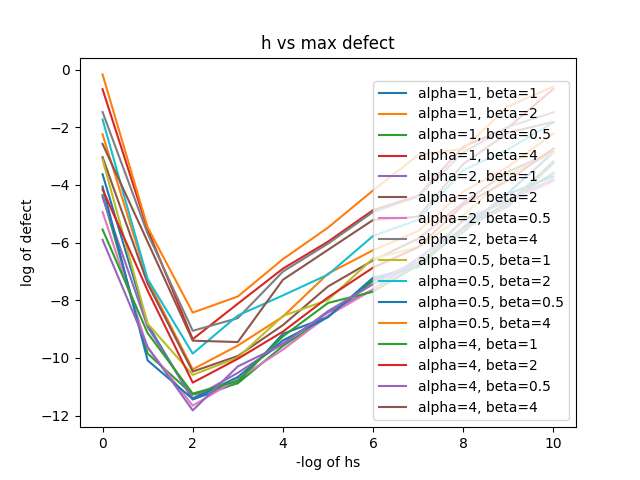
\includegraphics[width=0.7\linewidth]{./figures/hb10_alpha_beta_test}
\caption{HB10 - maximum size of the defect based on different values of $\alpha$ and $\beta$.}
\label{fig:hb10_alpha_beta_test}
\end{figure}


\paragraph{Results}
\paragraph{Problem 1 results}
Figures $\ref{fig:rk4_with_hb10_p1_global_defect}$, $\ref{fig:rk4_with_hb10_p1_global_error}$ and $\ref{fig:rk4_with_hb10_p1_scaled_defects}$ shows the results of using RK4 with HB10 on Problem 1. We note that an absolute tolerance of $10^{-6}$ is applied on the maximum defect within the step and this can be shown to occur at $0.3h$ and $0.8h$ along a step of size, h. See Figure $\ref{fig:rk4_with_hb10_p1_scaled_defects}$, to see the scaled defect reaching a maximum near these points. We note that we are able to successfully control the defect of the continuous numerical solution using this approach, see Figure $\ref{fig:rk4_with_hb10_p1_global_defect}$. 

\begin{figure}[H]
\centering
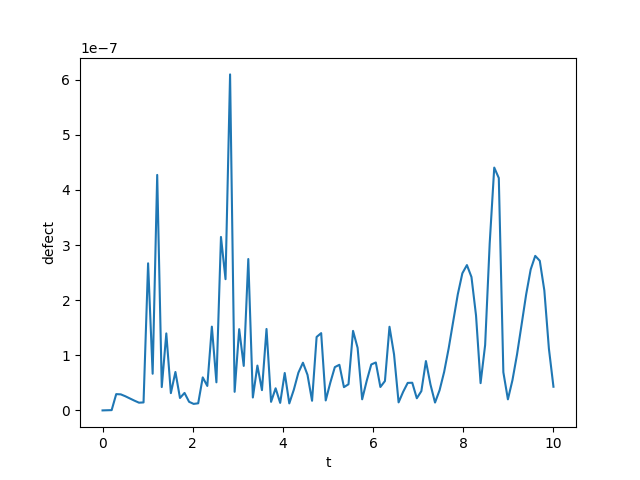
\includegraphics[width=0.7\linewidth]{./figures/rk4_with_hb10_p1_global_defect}
\caption{Defect across the entire domain for RK4 with HB10 on problem 1 at an absolute tolerance of $10^{-6}$.}
\label{fig:rk4_with_hb10_p1_global_defect}
\end{figure}

\begin{figure}[H]
\centering
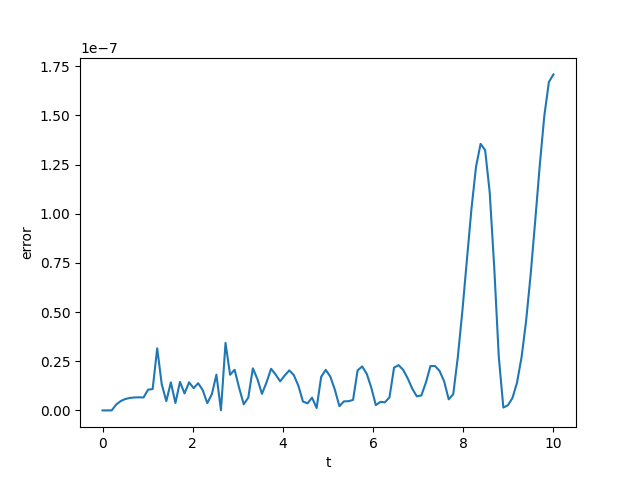
\includegraphics[width=0.7\linewidth]{./figures/rk4_with_hb10_p1_global_error}
\caption{Global Error for RK4 with HB10 on problem 1 at an absolute tolerance of $10^{-6}$.}
\label{fig:rk4_with_hb10_p1_global_error}
\end{figure}

\begin{figure}[H]
\centering
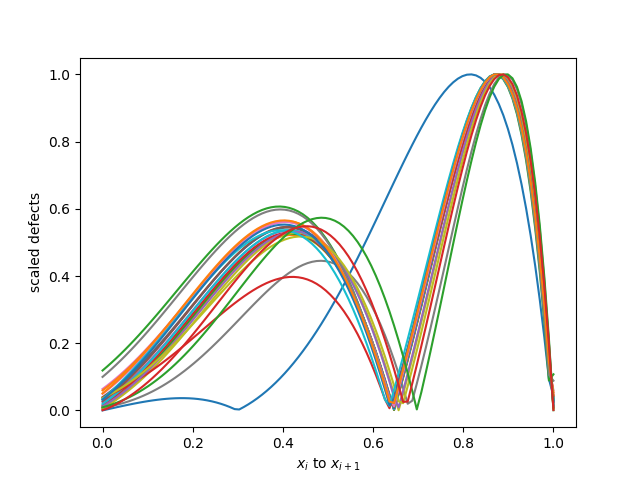
\includegraphics[width=0.7\linewidth]{./figures/rk4_with_hb10_p1_scaled_defects}
\caption{Scaled defects for RK4 with HB10 on problem 1 at an absolute tolerance of $10^{-6}$ mapped into $[0, 1]$.}
\label{fig:rk4_with_hb10_p1_scaled_defects}
\end{figure}

\paragraph{Problem 2 results}
Figures $\ref{fig:rk4_with_hb10_p2_global_defect}$, $\ref{fig:rk4_with_hb10_p2_global_error}$ and $\ref{fig:rk4_with_hb10_p2_scaled_defects}$ shows the results of using RK4 with HB10 on Problem 2. We note that an absolute tolerance of $10^{-6}$ is applied on the maximum defect within the step and this can be shown to occur at $0.8h$ along a step of size, h. See Figure $\ref{fig:rk4_with_hb10_p2_scaled_defects}$, to see the scaled defect reaching a maximum near these points. We note that we are able to successfully control the defect of the continuous numerical solution using this approach, see Figure $\ref{fig:rk4_with_hb10_p2_global_defect}$. 

\begin{figure}[H]
\centering
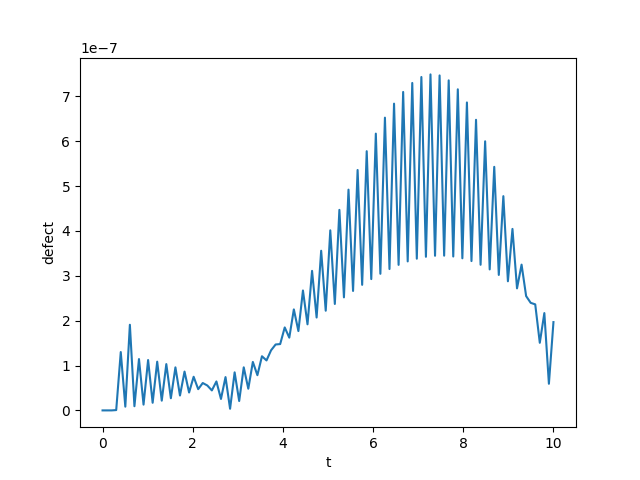
\includegraphics[width=0.7\linewidth]{./figures/rk4_with_hb10_p2_global_defect}
\caption{Defect across the entire domain for RK4 with HB10 on problem 2 at an absolute tolerance of $10^{-6}$.}
\label{fig:rk4_with_hb10_p2_global_defect}
\end{figure}

\begin{figure}[H]
\centering
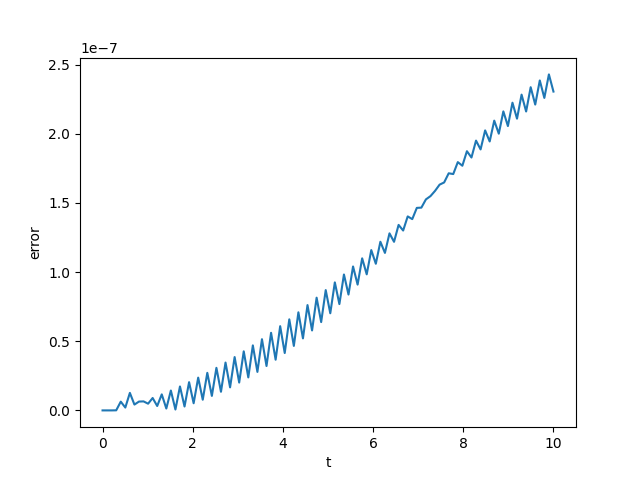
\includegraphics[width=0.7\linewidth]{./figures/rk4_with_hb10_p2_global_error}
\caption{Global Error for RK4 with HB10 on problem 2 at an absolute tolerance of $10^{-6}$.}
\label{fig:rk4_with_hb10_p2_global_error}
\end{figure}

\begin{figure}[H]
\centering
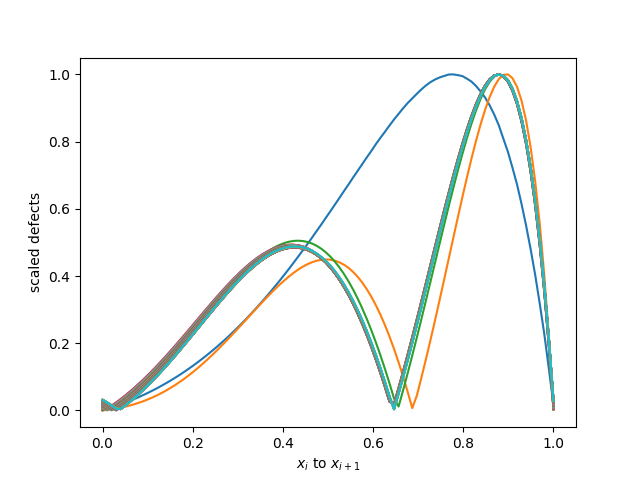
\includegraphics[width=0.7\linewidth]{./figures/rk4_with_hb10_p2_scaled_defects}
\caption{Scaled defects of RK4 with HB10 for problem 2 at an absolute tolerance of $10^{-6}$ mapped into $[0, 1]$.}
\label{fig:rk4_with_hb10_p2_scaled_defects}
\end{figure}

\paragraph{Problem 3 results}
Figures $\ref{fig:rk4_with_hb10_p3_global_defect}$, $\ref{fig:rk4_with_hb10_p3_global_error}$ and $\ref{fig:rk4_with_hb10_p3_scaled_defects}$ shows the results of using RK4 with HB10 on Problem 3. 
We note that an absolute tolerance of $10^{-6}$ is applied on the maximum defect within the step and this can be shown to occur at $0.3h$ or $0.8h$ along a step of size, h.  See Figure $\ref{fig:rk4_with_hb10_p3_scaled_defects}$, to see the scaled defect reaching a maximum near these points. We note that we are able to successfully control the defect of the continuous numerical solution using this approach, see Figure $\ref{fig:rk4_with_hb10_p3_global_defect}$. 

\begin{figure}[H]
\centering
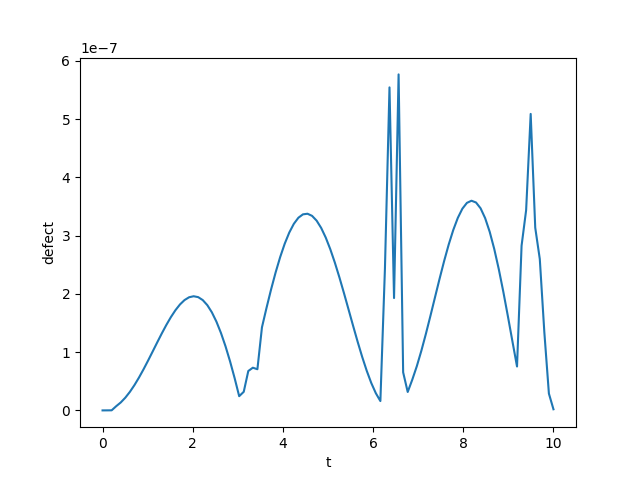
\includegraphics[width=0.7\linewidth]{./figures/rk4_with_hb10_p3_global_defect}
\caption{Defect across the entire domain of RK4 with HB10 on problem 3 at an absolute tolerance of $10^{-6}$.}
\label{fig:rk4_with_hb10_p3_global_defect}
\end{figure}

\begin{figure}[H]
\centering
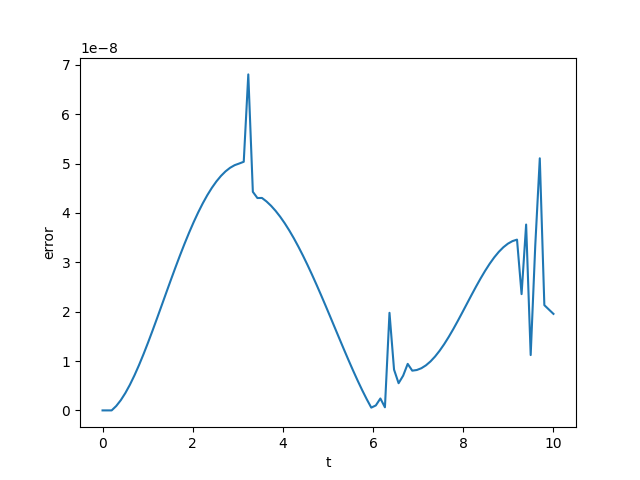
\includegraphics[width=0.7\linewidth]{./figures/rk4_with_hb10_p3_global_error}
\caption{Global Error of RK4 with HB10 on problem 3 at an absolute tolerance of $10^{-6}$.}
\label{fig:rk4_with_hb10_p3_global_error}
\end{figure}

\begin{figure}[H]
\centering
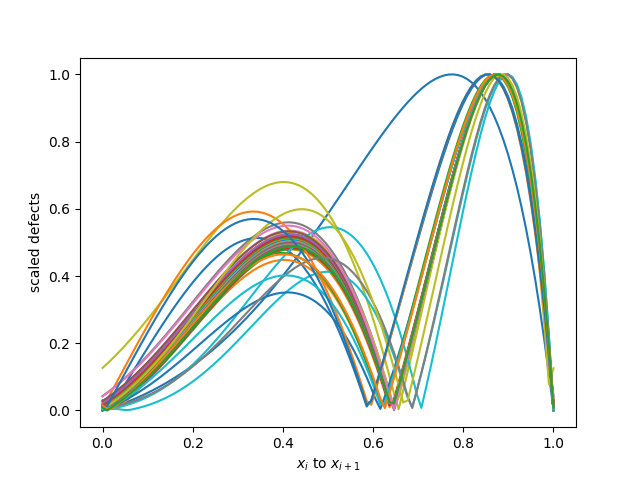
\includegraphics[width=0.7\linewidth]{./figures/rk4_with_hb10_p3_scaled_defects}
\caption{Scaled defects of RK4 with HB10 on problem 3 at an absolute tolerance of $10^{-6}$ mapped onto $[0, 1]$.}
\label{fig:rk4_with_hb10_p3_scaled_defects}
\end{figure}


\begin{table}[h]
\caption {Number of steps taken by RK4 when modified to do defect control with HB8 vs when modified with HB10.} \label{tab:rk4_with_hb10_nsteps}
\begin{center}
\begin{tabular}{ c c c c c } 
Problem & succ. steps HB8 & succ. steps HB10 & nsteps HB8 & nsteps HB10 \\ 
1       & 20                 &        24          & 20         & 25\\ 
2       & 37                 &        50          & 60         & 50\\
3       & 69                 &        93          & 89         & 97\\
\end{tabular}
\end{center}
\end{table}

HB10 seems to be worse than HB8. We will explain this in Section $\ref{section:crks_vs_hbs}$. This is because at coarser tolerance HB10 works worse than HB8. This is because though the order is $O(h^{10})$ versus $O(h^8)$, the coefficient for HB10 is much worse. Thus it is only when the step sizes are smaller that HB10 works better than HB8.




\section{Higher Order Runge Kutta Methods}
\label{section:HBs_and_higher_order_RK}
In this section, we attempt to perform defect control based on efficient multistep interpolants for higher order Runge-Kutta methods. We recall that related previous work used significantly more stages to obtain a continuous $6^{th}$ order Runge-Kutta method and a continuous $8^{th}$ order Runge-Kutta method.

In this section, we will first augment the RK6 method (see Section $\ref{section:basic_runge_kutta}$ for details about the discrete method) with HB6 and then with HB8. We hope to perform defect control and to find that the use of HB8 allows significantly fewer steps. We will then augment the RK8 method (see Section $\ref{section:basic_runge_kutta}$ for more details) with HB8 to show that though interpolation error is present, the scheme does allow defect control of a continuous $8^{th}$ order solution. 

For both methods, we will sample the defect only twice in a step, at $0.4h$ and $0.8h$ in a step of size $h$, as the previous experiments appears to indicate that the maximum defects tend to occur at these locations within each step.

\subsection{RK6 with HB6}
\paragraph{Problem 1 results}
Figures $\ref{fig:rk6_with_hb6_p1_global_defect}$, $\ref{fig:rk6_with_hb6_p1_global_error}$ and $\ref{fig:rk6_with_hb6_p1_scaled_defects}$ shows the results of using RK6 with HB6 on Problem 1. We note that an absolute tolerance of $10^{-6}$ is applied on the maximum defect within the step and this can be shown to occur at $0.3h$ and $0.8h$ along a step of size, h. See Figure $\ref{fig:rk6_with_hb6_p1_scaled_defects}$, to see the scaled defect reaching a maximum near these points. We note that we are able to successfully control the defect of the continuous numerical solution using this approach, see Figure $\ref{fig:rk6_with_hb6_p1_global_defect}$. 

\begin{figure}[H]
\centering
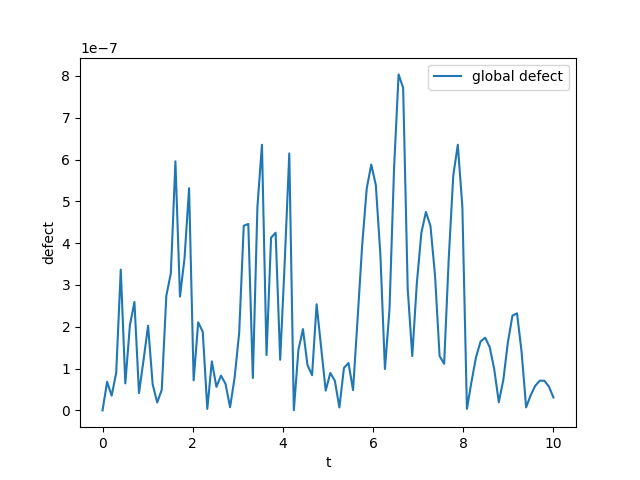
\includegraphics[width=0.7\linewidth]{./figures/rk6_with_hb6_p1_global_defect}
\caption{Defect across the entire domain for RK6 with HB6 on problem 1 at an absolute tolerance of $10^{-6}$.}
\label{fig:rk6_with_hb6_p1_global_defect}
\end{figure}

\begin{figure}[H]
\centering
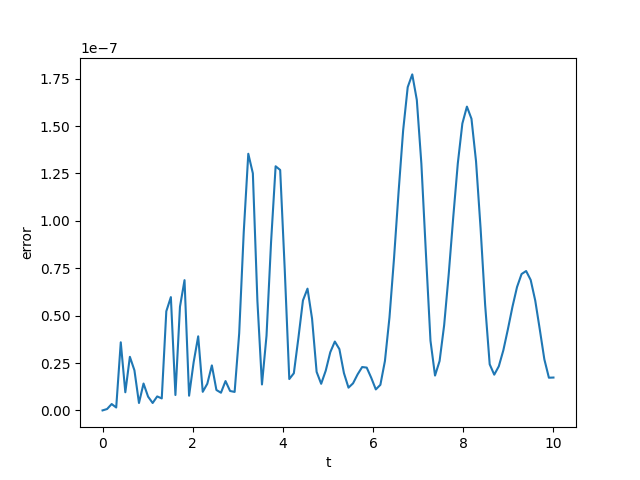
\includegraphics[width=0.7\linewidth]{./figures/rk6_with_hb6_p1_global_error}
\caption{Global Error for RK6 with HB6 on problem 1 at an absolute tolerance of $10^{-6}$.}
\label{fig:rk6_with_hb6_p1_global_error}
\end{figure}

\begin{figure}[H]
\centering
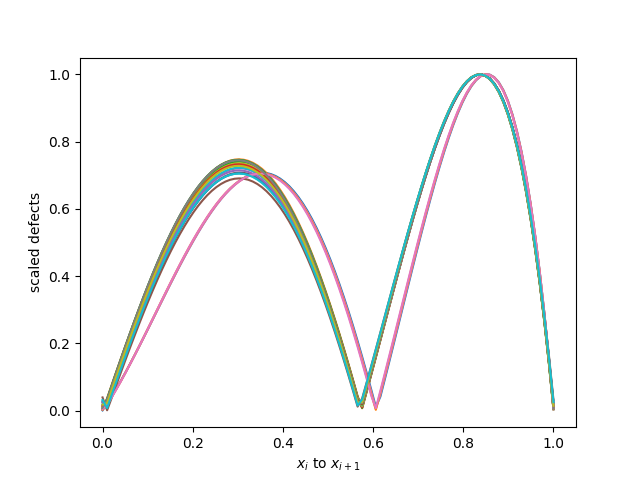
\includegraphics[width=0.7\linewidth]{./figures/rk6_with_hb6_p1_scaled_defects}
\caption{Scaled defects for RK6 with HB6 on problem 1 at an absolute tolerance of $10^{-6}$ mapped onto $[0, 1]$.}
\label{fig:rk6_with_hb6_p1_scaled_defects}
\end{figure}

\paragraph{Problem 2 results}
Figures $\ref{fig:rk6_with_hb6_p2_global_defect}$, $\ref{fig:rk6_with_hb6_p2_global_error}$ and $\ref{fig:rk6_with_hb6_p2_scaled_defects}$ shows the results of using RK6 with HB6 on Problem 2. We note that an absolute tolerance of $10^{-6}$ is applied on the maximum defect within the step and this can be shown to occur at $0.3h$ or $0.8h$ along a step of size, h. See Figure $\ref{fig:rk6_with_hb6_p2_scaled_defects}$, to see the scaled defect reaching a maximum near these points. We note that we are able to successfully control the defect of the continuous numerical solution using this approach, see Figure $\ref{fig:rk6_with_hb6_p2_global_defect}$. 

\begin{figure}[H]
\centering
\includegraphics[width=0.7\linewidth]{./figures/rk6_with_hb6_p2_global_defect}
\caption{Defect across the entire domain for RK6 with HB6 on problem 2 at an absolute tolerance of $10^{-6}$.}
\label{fig:rk6_with_hb6_p2_global_defect}
\end{figure}

\begin{figure}[H]
\centering
\includegraphics[width=0.7\linewidth]{./figures/rk6_with_hb6_p2_global_error}
\caption{Global Error for RK6 with HB6 on problem 2 at an absolute tolerance of $10^{-6}$.}
\label{fig:rk6_with_hb6_p2_global_error}
\end{figure}

\begin{figure}[H]
\centering
\includegraphics[width=0.7\linewidth]{./figures/rk6_with_hb6_p2_scaled_defects}
\caption{Scaled defects for RK6 with HB6 on problem 2 at an absolute tolerance of $10^{-6}$ mapped onto $[0, 1]$.}
\label{fig:rk6_with_hb6_p2_scaled_defects}
\end{figure}

\begin{figure}[H]
\centering
\includegraphics[width=0.7\linewidth]{./figures/rk6_with_hb6_p2_scaled_defects_small_steps}
\caption{Scaled defects for RK6 with HB6 on small steps on problem 2 at an absolute tolerance of $10^{-6}$ mapped onto $[0, 1]$. Despite the noise, for most steps, the maximum defect mostly appears near $0.8h$.}
\label{fig:rk6_with_hb6_p2_scaled_defects_small_steps}
\end{figure}

\paragraph{Problem 3 results}
Figures $\ref{fig:rk6_with_hb6_p3_global_defect}$, $\ref{fig:rk6_with_hb6_p3_global_error}$ and $\ref{fig:rk6_with_hb6_p3_scaled_defects}$ shows the results of using RK6 with HB6 on Problem 3. 
We note that an absolute tolerance of $10^{-6}$ is applied on the maximum defect within the step and this can be shown to occur at $0.3h$ or $0.8h$ along a step of size, h. See Figure $\ref{fig:rk6_with_hb6_p3_scaled_defects}$, to see the scaled defect reaching a maximum near these points. We note that we are able to successfully control the defect of the continuous numerical solution using this approach, see Figure $\ref{fig:rk6_with_hb6_p3_global_defect}$. 

\begin{figure}[H]
\centering
\includegraphics[width=0.7\linewidth]{./figures/rk6_with_hb6_p3_global_defect}
\caption{Defect across the entire domain for RK6 with HB6 on problem 3 at an absolute tolerance of $10^{-6}$.}
\label{fig:rk6_with_hb6_p3_global_defect}
\end{figure}

\begin{figure}[H]
\centering
\includegraphics[width=0.7\linewidth]{./figures/rk6_with_hb6_p3_global_error}
\caption{Global Error for RK6 with HB6 on problem 3 at an absolute tolerance of $10^{-6}$.}
\label{fig:rk6_with_hb6_p3_global_error}
\end{figure}

\begin{figure}[H]
\centering
\includegraphics[width=0.7\linewidth]{./figures/rk6_with_hb6_p3_scaled_defects}
\caption{Scaled defects for RK6 with HB6 on problem 3 at an absolute tolerance of $10^{-6}$ mapped onto $[0, 1]$.}
\label{fig:rk6_with_hb6_p3_scaled_defects}
\end{figure}

\begin{figure}[H]
\centering
\includegraphics[width=0.7\linewidth]{./figures/rk6_with_hb6_p3_scaled_defects_small_steps}
\caption{Scaled defects for RK6 with HB6 on small steps on problem 3 at an absolute tolerance of $10^{-6}$ mapped onto $[0, 1]$.}
\label{fig:rk6_with_hb6_p3_scaled_defects_small_steps}
\end{figure}

\subsection{RK6 with HB8}
\paragraph{Problem 1 results}
Figures $\ref{fig:rk6_with_hb8_p1_global_defect}$, $\ref{fig:rk6_with_hb8_p1_global_error}$ and $\ref{fig:rk6_with_hb8_p1_scaled_defects}$ shows the results of using RK6 with HB8 on Problem 1. We note that an absolute tolerance of $10^{-6}$ is applied on the maximum defect within the step and this can be shown to occur at $0.4h$ and $0.8h$ along a step of size, h. See Figure $\ref{fig:rk6_with_hb8_p1_scaled_defects}$, to see the scaled defect reaching a maximum near these points. We note that we are able to successfully control the defect of the continuous numerical solution using this approach, see Figure $\ref{fig:rk6_with_hb8_p1_global_defect}$. 


\begin{figure}[H]
\centering
\includegraphics[width=0.7\linewidth]{./figures/rk6_with_hb8_p1_global_defect}
\caption{Defect across the entire domain for RK6 with HB8 on problem 1 at an absolute tolerance of $10^{-6}$.}
\label{fig:rk6_with_hb8_p1_global_defect}
\end{figure}

\begin{figure}[H]
\centering
\includegraphics[width=0.7\linewidth]{./figures/rk6_with_hb8_p1_global_error}
\caption{Global Error for RK6 with HB8 on problem 1 at an absolute tolerance of $10^{-6}$.}
\label{fig:rk6_with_hb8_p1_global_error}
\end{figure}

\begin{figure}[H]
\centering
\includegraphics[width=0.7\linewidth]{./figures/rk6_with_hb8_p1_scaled_defects}
\caption{Scaled defects for RK6 with HB8 on problem 1 at an absolute tolerance of $10^{-6}$ mapped onto $[0, 1]$.}
\label{fig:rk6_with_hb8_p1_scaled_defects}
\end{figure}

\paragraph{Problem 2 results}
Figures $\ref{fig:rk6_with_hb8_p2_global_defect}$, $\ref{fig:rk6_with_hb8_p2_global_error}$ and $\ref{fig:rk6_with_hb8_p2_scaled_defects}$ shows the results of using RK6 with HB8 on Problem 2. We note that an absolute tolerance of $10^{-6}$ is applied on the maximum defect within the step and this can be shown to occur at $0.8h$ along a step of size, h. See Figure $\ref{fig:rk6_with_hb8_p2_scaled_defects}$, to see the scaled defect reaching a maximum near these points. We note that we are able to successfully control the defect of the continuous numerical solution using this approach, see Figure $\ref{fig:rk6_with_hb8_p2_global_defect}$. 


\begin{figure}[H]
\centering
\includegraphics[width=0.7\linewidth]{./figures/rk6_with_hb8_p2_global_defect}
\caption{Defect across the entire domain for RK6 with HB8 on problem 2 at an absolute tolerance of $10^{-6}$.}
\label{fig:rk6_with_hb8_p2_global_defect}
\end{figure}

\begin{figure}[H]
\centering
\includegraphics[width=0.7\linewidth]{./figures/rk6_with_hb8_p2_global_error}
\caption{Global Error for RK6 with HB8 on problem 2 at an absolute tolerance of $10^{-6}$.}
\label{fig:rk6_with_hb8_p2_global_error}
\end{figure}

\begin{figure}[H]
\centering
\includegraphics[width=0.7\linewidth]{./figures/rk6_with_hb8_p2_scaled_defects}
\caption{Scaled defects for RK6 with HB8 on problem 2 at an absolute tolerance of $10^{-6}$ mapped onto $[0, 1]$.}
\label{fig:rk6_with_hb8_p2_scaled_defects}
\end{figure}

\begin{figure}[H]
\centering
\includegraphics[width=0.7\linewidth]{./figures/rk6_with_hb8_p2_scaled_defects_small_steps}
\caption{Scaled defects for RK6 with HB8 on small steps on problem 2 at an absolute tolerance of $10^{-6}$ mapped onto $[0, 1]$. Despite the noise, the maximum defect mostly appears near $0.8h$.}
\label{fig:rk6_with_hb8_p2_scaled_defects_small_steps}
\end{figure}

\paragraph{Problem 3 results}
Figures $\ref{fig:rk6_with_hb8_p3_global_defect}$, $\ref{fig:rk6_with_hb8_p3_global_error}$ and $\ref{fig:rk6_with_hb8_p3_scaled_defects}$ shows the results of RK6 with HB8 on Problem 3. 
We note that an absolute tolerance of $10^{-6}$ is applied on the maximum defect within the step and this can be shown to occur at either $0.4h$ or $0.8h$ along a step of size, h. See Figure $\ref{fig:rk6_with_hb8_p3_scaled_defects}$, to see the scaled defect reaching a maximum near these points. We note that we are able to successfully control the defect of the continuous numerical solution using this approach, see Figure $\ref{fig:rk6_with_hb8_p3_global_defect}$. 
 

\begin{figure}[H]
\centering
\includegraphics[width=0.7\linewidth]{./figures/rk6_with_hb8_p3_global_defect}
\caption{Defect across the entire domain for RK6 with HB8 on problem 3 at an absolute tolerance of $10^{-6}$.}
\label{fig:rk6_with_hb8_p3_global_defect}
\end{figure}

\begin{figure}[H]
\centering
\includegraphics[width=0.7\linewidth]{./figures/rk6_with_hb8_p3_global_error}
\caption{Global Error for RK6 with HB8 on problem 3 at an absolute tolerance of $10^{-6}$.}
\label{fig:rk6_with_hb8_p3_global_error}
\end{figure}

\begin{figure}[H]
\centering
\includegraphics[width=0.7\linewidth]{./figures/rk6_with_hb8_p3_scaled_defects}
\caption{Scaled defects for RK6 with HB8 on problem 3 at an absolute tolerance of $10^{-6}$ mapped onto $[0, 1]$.}
\label{fig:rk6_with_hb8_p3_scaled_defects}
\end{figure}

\begin{figure}[H]
\centering
\includegraphics[width=0.7\linewidth]{./figures/rk6_with_hb8_p3_scaled_defects_small_steps}
\caption{Scaled defects for RK6 with HB8 on small steps on problem 3 at an absolute tolerance of $10^{-6}$ mapped onto $[0, 1]$. Despite the noise, the maximum defect mostly appears near $0.8h$.}
\label{fig:rk6_with_hb8_p3_scaled_defects_small_steps}
\end{figure}

\begin{table}[h]
\caption {Number of steps taken by RK6 when modified to do defect control with HB8 vs when modified with HB6.} \label{tab:rk6_with_hb6_vs_hb8_nsteps}
\begin{center}
\begin{tabular}{ c c c c c } 
Problem & succ. steps HB8 & succ. steps HB6 & nsteps HB8 & nsteps HB6 \\ 
1       & 18                 &        26          & 18         & 27\\ 
2       & 14                 &        18          & 17         & 23\\
3       & 24                 &        42          & 26         & 51\\
\end{tabular}
\end{center}
\end{table}

From Table $\ref{tab:rk6_with_hb6_vs_hb8_nsteps}$, we can see that again, using an interpolant whose interpolation error and especially the interpolation error of its derivative is of higher order than the ODE solution drastically reduces the number of steps. The solver becomes more efficient as a result. Since RK6 with HB6 and with HB8 is behaving similarly to RK4 with HB4 and with HB6, we expect that using a $10^{th}$ order method would not improve the situation more than HB8 has over HB6. Though fitting RK6 with HB10 will be as efficient as fitting it with HB8, the fact that the interpolation error is no longer the limiting factor means that HB10 will not improve the situation. For RK6, HB8 is the preferred interpolant.  

We also note that during the solving of the 3 problems, the value of $\alpha$ with HB6 rarely was bigger than 4 or smaller than $\frac{1}{4}$. The values of $\alpha$ and $\beta$ with HB8 also rarely were bigger than 4 or smaller than $\frac{1}{4}$. 

\subsection{RK8 with HB8}
In this section, we fit the RK8 method, described in Section $\ref{section:basic_runge_kutta}$, with HB8. Though we expect the interpolation error to reduce the efficiency of this scheme, we provide a proof of concept that an RK8 can have defect control with the scheme presented in this chapter. We will look into the challenges and possibilities of deriving an HB10 scheme in the Future Work section. 

\paragraph{Problem 1 results}
Figures $\ref{fig:rk8_with_hb8_p1_global_defect}$, $\ref{fig:rk8_with_hb8_p1_global_error}$ and $\ref{fig:rk8_with_hb8_p1_scaled_defects}$ shows the results of using RK8 with HB8 on Problem 1. We note that an absolute tolerance of $10^{-6}$ is applied on the maximum defect within the step and this can be shown to occur at $0.3h$ and $0.8h$ along a step of size, h. See Figure $\ref{fig:rk8_with_hb8_p1_scaled_defects}$, to see the scaled defect reaching a maximum near these points. We note that we are able to successfully control the defect of the continuous numerical solution using this approach, see Figure $\ref{fig:rk8_with_hb8_p1_global_defect}$. 
 

\begin{figure}[H]
\centering
\includegraphics[width=0.7\linewidth]{./figures/rk8_with_hb8_p1_global_defect}
\caption{Defect across the entire domain for RK8 with HB8 on problem 1 at an absolute tolerance of $10^{-6}$.}
\label{fig:rk8_with_hb8_p1_global_defect}
\end{figure}

\begin{figure}[H]
\centering
\includegraphics[width=0.7\linewidth]{./figures/rk8_with_hb8_p1_global_error}
\caption{Global Error for RK8 with HB8 on problem 1 at an absolute tolerance of $10^{-6}$.}
\label{fig:rk8_with_hb8_p1_global_error}
\end{figure}

\begin{figure}[H]
\centering
\includegraphics[width=0.7\linewidth]{./figures/rk8_with_hb8_p1_scaled_defects}
\caption{Scaled defects for RK8 with HB8 on problem 1 at an absolute tolerance of $10^{-6}$  mapped onto $[0, 1]$.}
\label{fig:rk8_with_hb8_p1_scaled_defects}
\end{figure}

\paragraph{Problem 2 results}
Figures $\ref{fig:rk8_with_hb8_p2_global_defect}$, $\ref{fig:rk8_with_hb8_p2_global_error}$ and $\ref{fig:rk8_with_hb8_p2_scaled_defects}$ shows the results of using RK8 with HB8 on Problem 2. We note that an absolute tolerance of $10^{-6}$ is applied on the maximum defect within the step and this can be shown to occur at $0.3h$ or $0.8h$ along a step of size, h. See Figure $\ref{fig:rk8_with_hb8_p2_scaled_defects}$, to see the scaled defect reaching a maximum near these points. We note that we are able to successfully control the defect of the continuous numerical solution using this approach, see Figure $\ref{fig:rk8_with_hb8_p2_global_defect}$. 

\begin{figure}[H]
\centering
\includegraphics[width=0.7\linewidth]{./figures/rk8_with_hb8_p2_global_defect}
\caption{Defect across the entire domain for RK8 with HB8 on problem 2 at an absolute tolerance of $10^{-6}$.}
\label{fig:rk8_with_hb8_p2_global_defect}
\end{figure}

\begin{figure}[H]
\centering
\includegraphics[width=0.7\linewidth]{./figures/rk8_with_hb8_p2_global_error}
\caption{Global Error for RK8 with HB8 on problem 2 at an absolute tolerance of $10^{-6}$.}
\label{fig:rk8_with_hb8_p2_global_error}
\end{figure}

\begin{figure}[H]
\centering
\includegraphics[width=0.7\linewidth]{./figures/rk8_with_hb8_p2_scaled_defects}
\caption{Scaled defects for RK8 with HB8 on problem 2 at an absolute tolerance of $10^{-6}$  mapped onto $[0, 1]$.}
\label{fig:rk8_with_hb8_p2_scaled_defects}
\end{figure}

\begin{figure}[H]
\centering
\includegraphics[width=0.7\linewidth]{./figures/rk8_with_hb8_p2_scaled_defects_small_steps}
\caption{Scaled defects of RK8 with HB8 on small steps on problem 2 at an absolute tolerance of $10^{-6}$ mapped onto $[0, 1]$. Despite the noise, the maximum defect mostly appears near $0.8h$.}
\label{fig:rk8_with_hb8_p2_scaled_defects_small_steps}
\end{figure}

\paragraph{Problem 3 results}
Figures $\ref{fig:rk8_with_hb8_p3_global_defect}$, $\ref{fig:rk8_with_hb8_p3_global_error}$ and $\ref{fig:rk8_with_hb8_p3_scaled_defects}$ shows the results of using the modification of RK8 with HB8 on Problem 3. 
We note that an absolute tolerance of $10^{-6}$ is applied on the maximum defect within the step and this can be shown to occur at $0.3h$ or $0.8h$ along a step of size, h. See Figure $\ref{fig:rk8_with_hb8_p3_scaled_defects}$, to see the scaled defect reaching a maximum near these points. We note that we are able to successfully control the defect of the continuous numerical solution using this approach, see Figure $\ref{fig:rk8_with_hb8_p3_global_defect}$. 


\begin{figure}[H]
\centering
\includegraphics[width=0.7\linewidth]{./figures/rk8_with_hb8_p3_global_defect}
\caption{Defect across the entire domain for RK8 with HB8 on problem 3 at an absolute tolerance of $10^{-6}$.}
\label{fig:rk8_with_hb8_p3_global_defect}
\end{figure}

\begin{figure}[H]
\centering
\includegraphics[width=0.7\linewidth]{./figures/rk8_with_hb8_p3_global_error}
\caption{Global Error for RK8 with HB8 on problem 3 at an absolute tolerance of $10^{-6}$.}
\label{fig:rk8_with_hb8_p3_global_error}
\end{figure}

\begin{figure}[H]
\centering
\includegraphics[width=0.7\linewidth]{./figures/rk8_with_hb8_p3_scaled_defects}
\caption{Scaled defects for RK8 with HB8 on problem 3 at an absolute tolerance of $10^{-6}$  mapped onto $[0, 1]$. Despite the noise, the maximum defect mostly appears near $0.8h$.}
\label{fig:rk8_with_hb8_p3_scaled_defects}
\end{figure}

\begin{figure}[H]
\centering
\includegraphics[width=0.7\linewidth]{./figures/rk8_with_hb8_p3_scaled_defects_small_steps}
\caption{Scaled Defects of RK8 with HB8 on small steps on problem 3 at an absolute tolerance of $10^{-6}$ mapped onto $[0, 1]$.}
\label{fig:rk8_with_hb8_p3_scaled_defects_small_steps}
\end{figure}

\begin{table}[h]
\caption {Number of steps taken by RK8 when modified to do defect control with HB8.} \label{tab:rk8_with_hb8_nsteps}
\begin{center}
\begin{tabular}{ c c c } 
Problem & succ. steps & nsteps \\ 
1       & 18             &        19 \\ 
2       & 12             &        15 \\
3       & 24             &        29 \\
\end{tabular}
\end{center}
\end{table}

\section{Using the previous interpolants to keep the weight parameters at 1}
\label{section:keeping_alpha_at_1}
One idea to solve the problem of the loss in accuracy due to deviation of the $\alpha$ and $\beta$ parameters from 1 is to construct the interpolant using a value of 1 for these parameters. We note that the best accuracy we can hope to get is with a value of 1 and thus employing data values situated at uniform distances apart guarantees the minimum error.

\paragraph{HB6} For the HB6 case, a simple way to guarantee that the value of $\alpha$ is 1 is by using the previous interpolants to get the required values at $x_{i - 1}=x_i - h$. Say we are at a value $x_i$ and we took a step of size $h$ to get to the value $x_{i + 1}$ where the function evaluation was $f_{i + 1}$ and the solution was $y_{i + 1}$. We could use the previous interpolants defined on the range $[0, x_i]$ to get a value at $x_i - h$ for the solution approximation, $y_{i - 1}$, and then we can use this $y_{i-1}$ value to compute $f(t_{i-1}, y_{i-1})$ to get the derivative $f_{i - 1}$.  We could thus create the new interpolant using these data points to guarantee that $\alpha$ stays at 1. This technique costs one extra function evaluation to obtain $f_{i-1}$.

This technique works (see Figures $\ref{fig:static_alpha_rk4_with_hb6_p1_global_defect}$ to $\ref{fig:static_alpha_rk4_with_hb6_p3_scaled_defects}$ to see the defect being controlled) but will require that the step-size is artificially limited on the first few steps so that we can interpolant back $x_i - h$ and still be in a range where our interpolants are correctly defined. For example, If we go from $t_0$ to $t_0 + h$ and the error estimate is much lower than the tolerance, we cannot use a step size of $2h$ as $t_0 + h - 2h$ = $t_0-h$ because we do not have an interpolant in the region $\leq t_0$. However this is not an issue as we can perform the first few steps with a CRK scheme for example.

\paragraph{Problem 1 results}
Figures $\ref{fig:static_alpha_rk4_with_hb6_p1_global_defect}$, $\ref{fig:static_alpha_rk4_with_hb6_p1_global_error}$ and $\ref{fig:static_alpha_rk4_with_hb6_p1_scaled_defects}$ shows the results of using the RK4 with HB6 and $\alpha = 1$ on Problem 1. We note that an absolute tolerance of $10^{-6}$ is applied on the maximum defect within the step and this can be shown to occur at $0.3h$ and $0.8h$ along a step of size, h. See Figure $\ref{fig:static_alpha_rk4_with_hb6_p1_scaled_defects}$, to see the scaled defect reaching a maximum near these points. We note that we are able to successfully control the defect of the continuous numerical solution using this approach, see Figure $\ref{fig:static_alpha_rk4_with_hb6_p1_global_defect}$. 


\begin{figure}[H]
\centering
\includegraphics[width=0.7\linewidth]{./figures/static_alpha_rk4_with_hb6_p1_global_defect}
\caption{Defect across the entire domain for RK4 with HB6 using $\alpha$ = 1 on problem 1 at an absolute tolerance of $10^{-6}$.}
\label{fig:static_alpha_rk4_with_hb6_p1_global_defect}
\end{figure}

\begin{figure}[H]
\centering
\includegraphics[width=0.7\linewidth]{./figures/static_alpha_rk4_with_hb6_p1_global_error}
\caption{Global Error for RK4 with HB6 using $\alpha$ = 1 on problem 1 at an absolute tolerance of $10^{-6}$.}
\label{fig:static_alpha_rk4_with_hb6_p1_global_error}
\end{figure}

\begin{figure}[H]
\centering
\includegraphics[width=0.7\linewidth]{./figures/static_alpha_rk4_with_hb6_p1_scaled_defects}
\caption{Scaled defects for RK4 with HB6 using $\alpha$ = 1 on problem 1 at an absolute tolerance of $10^{-6}$ mapped onto $[0, 1]$.}
\label{fig:static_alpha_rk4_with_hb6_p1_scaled_defects}
\end{figure}

\paragraph{Problem 2 results}
Figures $\ref{fig:static_alpha_rk4_with_hb6_p2_global_defect}$, $\ref{fig:static_alpha_rk4_with_hb6_p2_global_error}$ and $\ref{fig:static_alpha_rk4_with_hb6_p2_scaled_defects}$ shows the results of using RK4 with HB6 and $\alpha = 1$ on Problem 2. We note that an absolute tolerance of $10^{-6}$ is applied on the maximum defect within the step and this can be shown to occur at $0.8h$ along a step of size, h. See Figure $\ref{fig:static_alpha_rk4_with_hb6_p2_scaled_defects}$, to see the scaled defect reaching a maximum near these points. We note that we are able to successfully control the defect of the continuous numerical solution using this approach, see Figure $\ref{fig:static_alpha_rk4_with_hb6_p2_global_defect}$. 
\begin{figure}[H]
\centering
\includegraphics[width=0.7\linewidth]{./figures/static_alpha_rk4_with_hb6_p2_global_defect}
\caption{Defect across the entire domain for RK4 with HB6 using $\alpha$ = 1 on problem 2 at an absolute tolerance of $10^{-6}$.}
\label{fig:static_alpha_rk4_with_hb6_p2_global_defect}
\end{figure}

\begin{figure}[H]
\centering
\includegraphics[width=0.7\linewidth]{./figures/static_alpha_rk4_with_hb6_p2_global_error}
\caption{Global Error for RK4 with HB6 using $\alpha$ = 1 on problem 2 at an absolute tolerance of $10^{-6}$.}
\label{fig:static_alpha_rk4_with_hb6_p2_global_error}
\end{figure}

\begin{figure}[H]
\centering
\includegraphics[width=0.7\linewidth]{./figures/static_alpha_rk4_with_hb6_p2_scaled_defects}
\caption{Scaled defects for RK4 with HB6 using $\alpha$ = 1 on problem 2 at an absolute tolerance of $10^{-6}$ mapped onto $[0, 1]$.}
\label{fig:static_alpha_rk4_with_hb6_p2_scaled_defects}
\end{figure}

\begin{figure}[H]
\centering
\includegraphics[width=0.7\linewidth]{./figures/static_alpha_rk4_with_hb6_p2_scaled_defects_small_steps}
\caption{Scaled defects for RK4 with HB6 using $\alpha$ = 1 on small steps on problem 2 at an absolute tolerance of $10^{-6}$ mapped onto $[0, 1]$. Despite the noise, the maximum defect mostly appears near $0.8h$.}
\label{fig:static_alpha_rk4_with_hb6_p2_scaled_defects_small_steps}
\end{figure}

\paragraph{Problem 3 results}
Figures $\ref{fig:static_alpha_rk4_with_hb6_p3_global_defect}$, $\ref{fig:static_alpha_rk4_with_hb6_p3_global_error}$ and $\ref{fig:static_alpha_rk4_with_hb6_p3_scaled_defects}$ shows the results of using RK4 with HB6 and $\alpha = 1$ on Problem 3. We note that an absolute tolerance of $10^{-6}$ is applied on the maximum defect within the step and this can be shown to occur at $0.3h$ or $0.8h$along a step of size, h though this problem produces a more diverse location for the peaks. See Figure $\ref{fig:static_alpha_rk4_with_hb6_p3_scaled_defects}$, to see the scaled defect reaching a maximum near these points. We note that we are able to successfully control the defect of the continuous numerical solution using this approach, see Figure $\ref{fig:static_alpha_rk4_with_hb6_p3_global_defect}$. 

\begin{figure}[H]
\centering
\includegraphics[width=0.7\linewidth]{./figures/static_alpha_rk4_with_hb6_p3_global_defect}
\caption{Defect across the entire domain for RK4 with HB6 using $\alpha$ = 1 on problem 3 at an absolute tolerance of $10^{-6}$.}
\label{fig:static_alpha_rk4_with_hb6_p3_global_defect}
\end{figure}

\begin{figure}[H]
\centering
\includegraphics[width=0.7\linewidth]{./figures/static_alpha_rk4_with_hb6_p3_global_error}
\caption{Global Error for RK4 with HB6 using $\alpha$ = 1 on problem 3 at an absolute tolerance of $10^{-6}$.}
\label{fig:static_alpha_rk4_with_hb6_p3_global_error}
\end{figure}

\begin{figure}[H]
\centering
\includegraphics[width=0.7\linewidth]{./figures/static_alpha_rk4_with_hb6_p3_scaled_defects}
\caption{Scaled defects for RK4 with HB6 using $\alpha$ = 1 on problem 3 at an absolute tolerance of $10^{-6}$ mapped onto $[0, 1]$.}
\label{fig:static_alpha_rk4_with_hb6_p3_scaled_defects}
\end{figure}

\begin{table}[h]
\caption {Number of steps taken by RK4 when modified to do defect control with HB6 when we fix $\alpha$ at 1 vs when we allow it to fluctuate during the integration.} \label{tab:rk4_with_hb6_static_vs_variable_alpha}
\begin{center}
\begin{tabular}{ c c c c c } 
Problem & succ. steps & $\alpha$=1 succ. & nsteps & $\alpha$=1 nsteps \\ 
1       & 27                      &        29               & 27         & 33\\ 
2       & 36                      &        34               & 40         & 36\\
3       & 62                      &        65               & 73         & 82\\
\end{tabular}
\end{center}
\end{table}

Table $\ref{tab:rk4_with_hb6_static_vs_variable_alpha}$ shows how the solver with $\alpha$ fixed at 1 and the solver with $\alpha$ allowed to vary differ in the number of steps that they take. The results are very similar because, as we noted before, $\alpha$ tends to stay close to 1 and rarely deviates to a value smaller than $\frac{1}{4}$ or larger than 4.

\paragraph{HB8} For the HB8 case, a simple way to guarantee that the values of $\alpha$ and $\beta$ are 1 is by using the previous interpolants to get the required values at $x_{i - 1}=x_i-h$ and $x_{i - 2}=x_i-2h$. Suppose that we are at $x_i$ and we took a step of size $h$ to get to the value $x_{i + 1}$ where the function evaluation was $f_{i + 1}$ and the solution was $y_{i + 1}$. We could get the values of the solution and the derivative by using the previous interpolants defined on the range $[0, x_i]$ to get the value at exactly $x_i - h$ for the solution, $y_{i - 1}$, and then evaluate $f(t_{i-1}, y_{i-1})$ to get the derivative $f_{i - 1}$.  We can also use the previous interpolants on $[0, x_i]$ to get the values of the solution, $y_{i-2}$ and use it to evaluate $f(t_{i-2}, y_{i-2})$ to get the values of the derivative, $f_{i-2}$, at $x_{i-2} = x_i - 2h$. We could thus create create the new interpolant using the data values defined as such to guarantee that $\alpha$ and $\beta$ equal to 1. We note that we have built interpolants for both the solution and the derivative that  can interpolate up to $x_i$ for all cases except for the case $x_i = 0$ or for the first few steps. This scheme uses two more function evaluations.

This technique works (see Figures $\ref{fig:static_alpha_rk6_with_hb8_p1_global_defect}$ to $\ref{fig:static_alpha_rk6_with_hb8_p3_scaled_defects_small_steps}$ to see the defect being controlled) but will require that the step-size is artificially limited on the first few steps so that we can interpolant back $x_i - h$ and/or $x_i - 2h$ and still be in a range where our interpolants are correctly defined. This is not an issue as a CRK scheme could be used for the first few steps.

\paragraph{Problem 1 results}
Figures $\ref{fig:static_alpha_rk6_with_hb8_p1_global_defect}$, $\ref{fig:static_alpha_rk6_with_hb8_p1_global_error}$ and $\ref{fig:static_alpha_rk6_with_hb8_p1_scaled_defects}$ shows the results of using RK6 with HB8 and $\alpha = 1$ and $\beta = 1$ on Problem 1. We note that an absolute tolerance of $10^{-6}$ is applied on the maximum defect within the step and this can be shown to occur at $0.4h$ or $0.8h$ along a step of size, h. See Figure $\ref{fig:static_alpha_rk6_with_hb8_p1_scaled_defects}$, to see the scaled defect reaching a maximum near these points. We note that we are able to successfully control the defect of the continuous numerical solution using this approach, see Figure $\ref{fig:static_alpha_rk6_with_hb8_p1_global_defect}$. 
\begin{figure}[H]
\centering
\includegraphics[width=0.7\linewidth]{./figures/static_alpha_rk6_with_hb8_p1_global_defect}
\caption{Defect across the entire domain for RK6 with HB8 using $\alpha$ and $\beta$ = 1 on problem 1 at an absolute tolerance of $10^{-6}$.}
\label{fig:static_alpha_rk6_with_hb8_p1_global_defect}
\end{figure}

\begin{figure}[H]
\centering
\includegraphics[width=0.7\linewidth]{./figures/static_alpha_rk6_with_hb8_p1_global_error}
\caption{Global Error for RK6 with HB8 using $\alpha$ and $\beta$ = 1 on problem 1 at an absolute tolerance of $10^{-6}$.}
\label{fig:static_alpha_rk6_with_hb8_p1_global_error}
\end{figure}

\begin{figure}[H]
\centering
\includegraphics[width=0.7\linewidth]{./figures/static_alpha_rk6_with_hb8_p1_scaled_defects}
\caption{Scaled Defects for RK6 with HB8 using $\alpha$ and $\beta$ = 1 on problem 1 at an absolute tolerance of $10^{-6}$ mapped onto $[0, 1]$.}
\label{fig:static_alpha_rk6_with_hb8_p1_scaled_defects}
\end{figure}

\paragraph{Problem 2 results}
Figures $\ref{fig:static_alpha_rk6_with_hb8_p2_global_defect}$, $\ref{fig:static_alpha_rk6_with_hb8_p2_global_error}$ and $\ref{fig:static_alpha_rk6_with_hb8_p2_scaled_defects}$ shows the results of using RK6 with HB8 and $\alpha = 1$ and $\beta = 1$ on Problem 2. We note that an absolute tolerance of $10^{-6}$ is applied on the maximum defect within the step and this can be shown to occur at $0.8h$ along a step of size, h. See Figure $\ref{fig:static_alpha_rk6_with_hb8_p2_scaled_defects}$, to see the scaled defect reaching a maximum near these points. We note that we are able to successfully control the defect of the continuous numerical solution using this approach, see Figure $\ref{fig:static_alpha_rk6_with_hb8_p2_global_defect}$. 
\begin{figure}[H]
\centering
\includegraphics[width=0.7\linewidth]{./figures/static_alpha_rk6_with_hb8_p2_global_defect}
\caption{Defect across the entire domain for RK6 with HB8 using $\alpha$ and $\beta$ = 1 on problem 2 at an absolute tolerance of $10^{-6}$.}
\label{fig:static_alpha_rk6_with_hb8_p2_global_defect}
\end{figure}

\begin{figure}[H]
\centering
\includegraphics[width=0.7\linewidth]{./figures/static_alpha_rk6_with_hb8_p2_global_error}
\caption{Global Error for RK6 with HB8 using $\alpha$ and $\beta$ = 1 on problem 2 at an absolute tolerance of $10^{-6}$.}
\label{fig:static_alpha_rk6_with_hb8_p2_global_error}
\end{figure}

\begin{figure}[H]
\centering
\includegraphics[width=0.7\linewidth]{./figures/static_alpha_rk6_with_hb8_p2_scaled_defects}
\caption{Scaled Defects for RK6 with HB8 using $\alpha$ and $\beta$ = 1 on problem 2 at an absolute tolerance of $10^{-6}$ mapped onto $[0, 1]$.}
\label{fig:static_alpha_rk6_with_hb8_p2_scaled_defects}
\end{figure}

\begin{figure}[H]
\centering
\includegraphics[width=0.7\linewidth]{./figures/static_alpha_rk6_with_hb8_p2_scaled_defects_small_steps}
\caption{Scaled Defects for RK6 with HB8 using $\alpha$ and $\beta$ = 1 on small steps on problem 2 at an absolute tolerance of $10^{-6}$ mapped onto $[0, 1]$. Despite the noise, the maximum defect mostly appears near $0.8h$.}
\label{fig:static_alpha_rk6_with_hb8_p2_scaled_defects_small_steps}
\end{figure}

\paragraph{Problem 3 results}
Figures $\ref{fig:static_alpha_rk6_with_hb8_p3_global_defect}$, $\ref{fig:static_alpha_rk6_with_hb8_p3_global_error}$ and $\ref{fig:static_alpha_rk6_with_hb8_p3_scaled_defects}$ shows the results of using RK6 with HB8 and $\alpha = 1$ and $\beta = 1$ on Problem 3. We note that an absolute tolerance of $10^{-6}$ is applied on the maximum defect within the step and this can be shown to occur at $0.3h$ and $0.8h$ along a step of size, h. See Figure $\ref{fig:static_alpha_rk6_with_hb8_p3_scaled_defects}$, to see the scaled defect reaching a maximum near these points. We note that we are able to successfully control the defect of the continuous numerical solution using this approach, see Figure $\ref{fig:static_alpha_rk6_with_hb8_p3_global_defect}$. 

\begin{figure}[H]
\centering
\includegraphics[width=0.7\linewidth]{./figures/static_alpha_rk4_with_hb6_p3_global_defect}
\caption{Defect across the entire domain for RK6 with HB8 using $\alpha$ and $\beta$ = 1 on problem 3 at an absolute tolerance of $10^{-6}$.}
\label{fig:static_alpha_rk6_with_hb8_p3_global_defect}
\end{figure}

\begin{figure}[H]
\centering
\includegraphics[width=0.7\linewidth]{./figures/static_alpha_rk6_with_hb8_p3_global_error}
\caption{Global Error for RK6 with HB8 using $\alpha$ and $\beta$ = 1 on problem 3 at an absolute tolerance of $10^{-6}$.}
\label{fig:static_alpha_rk6_with_hb8_p3_global_error}
\end{figure}

\begin{figure}[H]
\centering
\includegraphics[width=0.7\linewidth]{./figures/static_alpha_rk6_with_hb8_p3_scaled_defects}
\caption{Scaled Defects for RK6 with HB8 using $\alpha$ and $\beta$ = 1 on problem 3 at an absolute tolerance of $10^{-6}$ mapped onto $[0, 1]$.}
\label{fig:static_alpha_rk6_with_hb8_p3_scaled_defects}
\end{figure}

\begin{figure}[H]
\centering
\includegraphics[width=0.7\linewidth]{./figures/static_alpha_rk6_with_hb8_p3_scaled_defects_small_steps}
\caption{Scaled Defects for RK6 with HB8 using $\alpha$ and $\beta$ = 1 on small steps on problem 3 at an absolute tolerance of $10^{-6}$ mapped onto $[0, 1]$. Despite the noise, the maximum defect mostly appears near $0.8h$.}
\label{fig:static_alpha_rk6_with_hb8_p3_scaled_defects_small_steps}
\end{figure}

\begin{table}[h]
\caption {Number of steps taken by RK6 when modified to do defect control with HB8 with $\alpha$ and $\beta$ forcibly at 1 and variable $\alpha$ and $\beta$.} \label{tab:rk6_with_hb8_static_vs_variable}
\begin{center}
\begin{tabular}{ c c c c c } 
Problem & succ. & params=1 succ. steps & nsteps & params=1 nsteps \\ 
1       & 18                      &        23               & 18         & 31\\ 
2       & 14                      &        18               & 17         & 21\\
3       & 24                      &        26               & 26         & 27\\
\end{tabular}
\end{center}
\end{table}	

Table $\ref{tab:rk6_with_hb8_static_vs_variable}$ shows how the solver with $\alpha$ and $\beta$ fixed at 1 and the solver with $\alpha$ and $\beta$ allowed to vary differs in the number of steps that they take. The results are somewhat similar because, as we noted before, $\alpha$ and $\beta$ tends to stay close to 1 and rarely deviates to a value smaller than $\frac{1}{4}$ or larger than 4.






\section{Final recommendations}
\label{section:final_recommendations_defect_control}
\subsection{The Vshaped graph and dependence on unit weight parameters}
\label{section:v_shaped_graph}
As we have shown several times in this thesis, the maximum order of accuracy of an interpolant depends on the value of the parameter $\alpha$ for the HB6 case and $\alpha$ and $\beta$ in the HB8 case. Furthermore, the accuracy also follows a V-shape as the interpolation error for sufficiently small $h$ reaches the round-off error. This is because the derivative of the interpolant uses a term in O($\frac{1}{h})$ where $h$ is the step-size. In this section we will look into how much these issues affect our interpolation. 

\paragraph{HB4}
In HB4, the error across several problems, across several sampling points, and at different step-sizes is as shown in Figure $\ref{fig:v_shape_across_problems_hb4}$. We note that this is without any parameters and at each h and each point $x$, we sampled at $x$ and $x + h$ to create the interpolant. The scheme suffers from an $O(\frac{1}{h})$ rounding off error inherently.
\begin{figure}[H]
\centering
\includegraphics[width=0.7\linewidth]{./figures/v_shape_across_problems_hb4}
\caption{V-shape of HB4 across problems at several sampling points and with h.}
\label{fig:v_shape_across_problems_hb4}
\end{figure}

We note that there is a clear optimal $h$ at about $10^{-3}$ and that we are able to achieve a tolerance of  $10^{-14}$ with some problems and $10^{-12}$ with almost every other problem. This gives us hope that this scheme can be used at very sharp tolerances. In this section, we will try several techniques to improve the situation. 


\paragraph{HB6}
In HB6, the error across several problems, across several sampling points, and at different step-sizes is as shown in Figure $\ref{fig:v_shape_across_problems_hb6}$. We note that that the parameter $\alpha$ is constant at 1 throughout the whole process as we sample at the point, $x$ and the points $x+h$ and $x-h$. This is the ideal case as the interpolation error is thus minimised.

\begin{figure}[H]
\centering
\includegraphics[width=0.7\linewidth]{./figures/v_shape_across_problems_hb6}
\caption{V-shape of HB6 across problems at several sampling points and with h.}
\label{fig:v_shape_across_problems_hb6}
\end{figure}

We note that $\alpha$ was kept at 1 in Figure $\ref{fig:v_shape_across_problems_hb6}$. To see how the parameter $\alpha$ reduces the accuracy as it deviates from 1, see Figure $\ref{fig:hb6_alpha_v_shape}$.

We can see that the optimal $h$ is at around $10^{-2}$. We note that in most cases we were able to reach an error of $10^{-14}$ but in some cases we were only able to solve at $10^{-12}$. 


\paragraph{HB8}
In HB8, the error across several problems, across several sampling points, and at different step-sizes is as shown in Figure $\ref{fig:v_shape_across_problems_hb8}$. We note that that both parameters $\alpha$ and $\beta$ were constant at 1 throughout the whole process as we sample at the point, $x$ and the points $x+h$, $x-h$ and $x-2h$. This is the ideal case as the interpolation error is thus minimised. 

\begin{figure}[H]
\centering
\includegraphics[width=0.7\linewidth]{./figures/v_shape_across_problems_hb8}
\caption{V-shape of HB8 across problems at several sampling points and with h.}
\label{fig:v_shape_across_problems_hb8}
\end{figure}

We note that both $\alpha$ and $\beta$ were kept at 1 in Figure $\ref{fig:v_shape_across_problems_hb8}$. To see how the parameters $\alpha$ and $\beta$ reduces the accuracy as it deviates from 1, see Figure $\ref{fig:hb8_second_scheme_alpha_beta_test}$.

We can see that the optimal $h$ is at around $10^{-1}$ and $10^{-2}$. We note that in most cases we were able to reach an error of $10^{-14}$ but in some cases we were only able to solve at $10^{-13}$. 

\subsection{Horner's and Barycentric interpolants to get to lower tolerances.}
\label{section:horner_bary_forms}
We note that up to this form, we have been using the monomial form of each of the cubic, quintic and septic polynomials that we have derived. In the previous section, we have shown how these were suffering from being eventually dominated by the rounding-off error as we use smaller and smaller step-sizes. One idea to deal with the loss of accuracy due to the interference from the rounding-off error is to use a different representation of the polynomials. 

One idea is to use the Horner's form of the polynomials. The Horner's form of a polynomial minimises the number of multiplications that need to be undertaken during the evaluation. It is faster and also a less prone to rounding-off errors since fewer arithmetic operations are involved.

Another idea is to use a Barycentric interpolant. At the time of the creation of the interpolant, if it is of order $n$ over the interval $[a, b]$, we can find $n$ Chebyshev points in the interval and then sample the interpolant at these $n$ points and then fit a Barycentric interpolant to these data points. A Barycentric interpolant using $n$ data points is of order $n$ and if such an interpolant is used to interpolate a polynomial of order $n$, it perfectly matches the polynomial that is, this process gives a different but exact representation of the original polynomial. The Chebyshev points are used to guarantee the minimum interpolation error.

We will use these two interpolation schemes to supplement the Hermite Birkhoff interpolants HB4, HB6 and HB8 at a few different sampling points at different problems and report on the improvements that they give.

\begin{figure}[H]
\centering
\includegraphics[width=0.7\linewidth]{./figures/typical_interp_horner_bary_hb4}
\caption{Typical plot of the HB4 interpolant monomial form vs the Horner form vs the Barycentric form.}
\label{fig:typical_interp_horner_bary_hb4}
\end{figure}

Figure $\ref{fig:typical_interp_horner_bary_hb4}$ shows a typical plot of HB4 in the monomial form alongside its Horner form and Barycentric interpolation forms. We can report that the Horner form almost always matches the accuracy of the interpolant but that the Barycentric form slightly improves the accuracy. The V-shape is inevitable as both forms either themselves suffer from $O(\frac{1}{h})$ rounding-off error or interpolate over an interpolant that suffers from such a rounding-off error.

\begin{figure}[H]
\centering
\includegraphics[width=0.7\linewidth]{./figures/typical_interp_horner_bary_hb6}
\caption{Typical plot of the HB6 interpolant monomial form vs the Horner form vs the Barycentric form.}
\label{fig:typical_interp_horner_bary_hb6}
\end{figure}

Figure $\ref{fig:typical_interp_horner_bary_hb6}$ shows a typical plot of HB6 in the monomial form alongside its Horner form and Barycentric interpolation forms. We note that the parameter $\alpha$ is kept at 1 in the above plot. We can report that the Horner form almost always matches the accuracy of the interpolant but that the Barycentric form slightly improves the accuracy. The V-shape is inevitable as both forms either themselves suffer from $O(\frac{1}{h})$ rounding-off error or interpolate over an interpolant that suffers from such a rounding-off error.

\begin{figure}[H]
\centering
\includegraphics[width=0.7\linewidth]{./figures/typical_interp_horner_bary_hb8}
\caption{Typical plot of the HB8 interpolant monomial form vs the Horner form vs the Barycentric form.}
\label{fig:typical_interp_horner_bary_hb8}
\end{figure}

Figure $\ref{fig:typical_interp_horner_bary_hb8}$ shows the typical plot of HB6 in the monomial form alongside its Horner form and Barycentric interpolation forms. We note that the parameters $\alpha$ and $\beta$ are kept at 1 in the above plot. For the case of HB8, the use of the Horner method or even the Barycentric method does not improve the situation. The monomial form is as accurate as we can get. The V-shape is inevitable as both forms either themselves suffer from $O(\frac{1}{h})$ rounding-off error or interpolate over an interpolant that suffers from such a rounding-off error.

\label{section:defect_final_recommendations}
As we have noted before, all the interpolants have a V-shaped defect. We should note that experimentally, the trough for these V-shapes seem to be problem-independent. We thus used the optimal $h$ value, that is the $h$ value where the minimum maximum defect is found, as the initial $h$ value for each solver. We need this, especially in the variable parameter case, so that the first few steps are accepted. These optimal values are as follows. For HB4, the optimal $h$ value seems to be at about $10^{-3}$, for HB6, the optimal $h$ value seems to be at around $10^{-2}$ and for HB8, the optimal value seems to be at around $10^{-1}$ and $10^{-2}$. See Appendix $\ref{section:v_shaped_graph}$ for more details.

We also experimented with using representations of the polynomials other than the monomial form to reduce the effect of the rounding-off error. We can look to use the Barycentric or Horner form of the polynomials to improve the accuracy for example. (See Appendix $\ref{section:horner_bary_forms}$ for more details.)

Some recommendations for a final solver will be to start with the optimal h for the respective interpolant as the first step size so that the $\alpha$ and $\beta$ parameters do not get too large or too small for the first steps. In an ideal case, we would like to keep accepting steps at the start and allow the parameters to be close to 1 for as long as possible.

We should solve with a solver with variable $\alpha$ at the start and then if the solver fails too many step repeatedly, that is, the parameters get too far from 1, we should use the technique of forcing the parameters to be 1 and using the previous interpolants.

The first recommendation guarantees that the first few steps are taken at the minimum error possible and thus that they succeed. The second recommendation guarantees that if we meet a challenging behaviour at some point, we would be able to step through it with static parameters at the cost of additional function evaluations.

We note that because of the V-shape, there is a high likelihood that we cannot solve any problem at very sharp tolerances (as sharper as $10^{-12}$). However, as have shown in Appendix $\ref{section:solving_at_sharp_tolerances}$, the solvers that were created were able to solve for tolerances of $2.5 \times 10^{-12}$.

% \appendix
\section{Recommendation for applying defect control at sharp tolerances}
\label{section:HBs_higher_tol}
\subsection{The Vshaped graph and dependence on unit weight parameters}
\label{section:v_shaped_graph}
As we have shown several times in this thesis, the maximum order of accuracy of an interpolant depends on the value of the parameter $\alpha$ for the HB6 case and $\alpha$ and $\beta$ in the HB8 case. Furthermore, the accuracy also follows a V-shape as the interpolation error for sufficiently small $h$ reaches the round-off error. This is because the derivative of the interpolant uses a term in O($\frac{1}{h})$ where $h$ is the step-size. In this section we will look into how much these issues affect our interpolation. 

\paragraph{HB4}
In HB4, the error across several problems, across several sampling points, and at different step-sizes is as shown in Figure $\ref{fig:v_shape_across_problems_hb4}$. We note that this is without any parameters and at each h and each point $x$, we sampled at $x$ and $x + h$ to create the interpolant. The scheme suffers from an $O(\frac{1}{h})$ rounding off error inherently.
\begin{figure}[H]
\centering
\includegraphics[width=0.7\linewidth]{./figures/v_shape_across_problems_hb4}
\caption{V-shape of HB4 across problems at several sampling points and with h.}
\label{fig:v_shape_across_problems_hb4}
\end{figure}

We note that there is a clear optimal $h$ at about $10^{-3}$ and that we are able to achieve a tolerance of  $10^{-14}$ with some problems and $10^{-12}$ with almost every other problem. This gives us hope that this scheme can be used at very sharp tolerances. In this section, we will try several techniques to improve the situation. 


\paragraph{HB6}
In HB6, the error across several problems, across several sampling points, and at different step-sizes is as shown in Figure $\ref{fig:v_shape_across_problems_hb6}$. We note that that the parameter $\alpha$ is constant at 1 throughout the whole process as we sample at the point, $x$ and the points $x+h$ and $x-h$. This is the ideal case as the interpolation error is thus minimised.

\begin{figure}[H]
\centering
\includegraphics[width=0.7\linewidth]{./figures/v_shape_across_problems_hb6}
\caption{V-shape of HB6 across problems at several sampling points and with h.}
\label{fig:v_shape_across_problems_hb6}
\end{figure}

We note that $\alpha$ was kept at 1 in Figure $\ref{fig:v_shape_across_problems_hb6}$. To see how the parameter $\alpha$ reduces the accuracy as it deviates from 1, see Figure $\ref{fig:hb6_alpha_v_shape}$.

We can see that the optimal $h$ is at around $10^{-2}$. We note that in most cases we were able to reach an error of $10^{-14}$ but in some cases we were only able to solve at $10^{-12}$. 


\paragraph{HB8}
In HB8, the error across several problems, across several sampling points, and at different step-sizes is as shown in Figure $\ref{fig:v_shape_across_problems_hb8}$. We note that that both parameters $\alpha$ and $\beta$ were constant at 1 throughout the whole process as we sample at the point, $x$ and the points $x+h$, $x-h$ and $x-2h$. This is the ideal case as the interpolation error is thus minimised. 

\begin{figure}[H]
\centering
\includegraphics[width=0.7\linewidth]{./figures/v_shape_across_problems_hb8}
\caption{V-shape of HB8 across problems at several sampling points and with h.}
\label{fig:v_shape_across_problems_hb8}
\end{figure}

We note that both $\alpha$ and $\beta$ were kept at 1 in Figure $\ref{fig:v_shape_across_problems_hb8}$. To see how the parameters $\alpha$ and $\beta$ reduces the accuracy as it deviates from 1, see Figure $\ref{fig:hb8_second_scheme_alpha_beta_test}$.

We can see that the optimal $h$ is at around $10^{-1}$ and $10^{-2}$. We note that in most cases we were able to reach an error of $10^{-14}$ but in some cases we were only able to solve at $10^{-13}$. 

\subsection{Horner's and Barycentric interpolants to get to lower tolerances.}
\label{section:horner_bary_forms}
We note that up to this form, we have been using the monomial form of each of the cubic, quintic and septic polynomials that we have derived. In the previous section, we have shown how these were suffering from being eventually dominated by the rounding-off error as we use smaller and smaller step-sizes. One idea to deal with the loss of accuracy due to the interference from the rounding-off error is to use a different representation of the polynomials. 

One idea is to use the Horner's form of the polynomials. The Horner's form of a polynomial minimises the number of multiplications that need to be undertaken during the evaluation. It is faster and also a less prone to rounding-off errors since fewer arithmetic operations are involved.

Another idea is to use a Barycentric interpolant. At the time of the creation of the interpolant, if it is of order $n$ over the interval $[a, b]$, we can find $n$ Chebyshev points in the interval and then sample the interpolant at these $n$ points and then fit a Barycentric interpolant to these data points. A Barycentric interpolant using $n$ data points is of order $n$ and if such an interpolant is used to interpolate a polynomial of order $n$, it perfectly matches the polynomial that is, this process gives a different but exact representation of the original polynomial. The Chebyshev points are used to guarantee the minimum interpolation error.

We will use these two interpolation schemes to supplement the Hermite Birkhoff interpolants HB4, HB6 and HB8 at a few different sampling points at different problems and report on the improvements that they give.

\begin{figure}[H]
\centering
\includegraphics[width=0.7\linewidth]{./figures/typical_interp_horner_bary_hb4}
\caption{Typical plot of the HB4 interpolant monomial form vs the Horner form vs the Barycentric form.}
\label{fig:typical_interp_horner_bary_hb4}
\end{figure}

Figure $\ref{fig:typical_interp_horner_bary_hb4}$ shows a typical plot of HB4 in the monomial form alongside its Horner form and Barycentric interpolation forms. We can report that the Horner form almost always matches the accuracy of the interpolant but that the Barycentric form slightly improves the accuracy. The V-shape is inevitable as both forms either themselves suffer from $O(\frac{1}{h})$ rounding-off error or interpolate over an interpolant that suffers from such a rounding-off error.

\begin{figure}[H]
\centering
\includegraphics[width=0.7\linewidth]{./figures/typical_interp_horner_bary_hb6}
\caption{Typical plot of the HB6 interpolant monomial form vs the Horner form vs the Barycentric form.}
\label{fig:typical_interp_horner_bary_hb6}
\end{figure}

Figure $\ref{fig:typical_interp_horner_bary_hb6}$ shows a typical plot of HB6 in the monomial form alongside its Horner form and Barycentric interpolation forms. We note that the parameter $\alpha$ is kept at 1 in the above plot. We can report that the Horner form almost always matches the accuracy of the interpolant but that the Barycentric form slightly improves the accuracy. The V-shape is inevitable as both forms either themselves suffer from $O(\frac{1}{h})$ rounding-off error or interpolate over an interpolant that suffers from such a rounding-off error.

\begin{figure}[H]
\centering
\includegraphics[width=0.7\linewidth]{./figures/typical_interp_horner_bary_hb8}
\caption{Typical plot of the HB8 interpolant monomial form vs the Horner form vs the Barycentric form.}
\label{fig:typical_interp_horner_bary_hb8}
\end{figure}

Figure $\ref{fig:typical_interp_horner_bary_hb8}$ shows the typical plot of HB6 in the monomial form alongside its Horner form and Barycentric interpolation forms. We note that the parameters $\alpha$ and $\beta$ are kept at 1 in the above plot. For the case of HB8, the use of the Horner method or even the Barycentric method does not improve the situation. The monomial form is as accurate as we can get. The V-shape is inevitable as both forms either themselves suffer from $O(\frac{1}{h})$ rounding-off error or interpolate over an interpolant that suffers from such a rounding-off error.

\subsection{Solving at sharp tolerances}
\label{section:solving_at_sharp_tolerances}
Using the recommendations, we show that the scheme can be used at very sharp tolerances for RK4 with HB6 and RK6 with HB8. In the plots below, we do not employ the switch from variable parameters to static parameters as they are not needed. The first few steps are all necessarily small and thus do not go out of range. The initial $h$ value is the experimental optimal $h$ value and we use the static parameters solvers. 

\subsubsection{RK4 with HB6}
\paragraph{Problem 1 results}
Figures $\ref{fig:sharp_tolerance_rk4_with_hb6_p1_global_defect}$, $\ref{fig:sharp_tolerance_rk4_with_hb6_p1_global_error}$ and $\ref{fig:sharp_tolerance_rk4_with_hb6_p1_scaled_defects}$ shows the results of using RK4 with HB6 and some of the recommendations on Problem 1. We note that an absolute tolerance of $2.5 \times 10^{-12}$ is applied on the maximum defect within the step and this can be shown to occur at $0.2h$ and $0.8h$ along a step of size, h. See Figure $\ref{fig:sharp_tolerance_rk4_with_hb6_p1_scaled_defects}$, to see the scaled defect reaching a maximum near these points. We note that we are able to successfully control the defect of the continuous numerical solution using this approach, see Figure $\ref{fig:sharp_tolerance_rk4_with_hb6_p1_global_defect}$. 

\begin{figure}[H]
\centering
\includegraphics[width=0.7\linewidth]{./figures/sharp_tolerance_rk4_with_hb6_p1_global_defect}
\caption{Defect across entire domain for RK4 with HB6 using $\alpha = 1$ and optimal h as the starting h value on problem 1 at an absolute tolerance of $2.5 \times 10^{-12}$.}
\label{fig:sharp_tolerance_rk4_with_hb6_p1_global_defect}
\end{figure}

\begin{figure}[H]
\centering
\includegraphics[width=0.7\linewidth]{./figures/sharp_tolerance_rk4_with_hb6_p1_global_error}
\caption{Global Error for RK4 with HB6 using $\alpha = 1$ and optimal h as the starting h value on problem 1 at an absolute tolerance of $2.5 \times 10^{-12}$.}
\label{fig:sharp_tolerance_rk4_with_hb6_p1_global_error}
\end{figure}

\begin{figure}[H]
\centering
\includegraphics[width=0.7\linewidth]{./figures/sharp_tolerance_rk4_with_hb6_p1_scaled_defects}
\caption{Scaled Defects for RK4 with HB6 using $\alpha = 1$ and optimal h as the starting h value on problem 1 at an absolute tolerance of $2.5 \times 10^{-12}$ mapped onto $[0, 1]$.}
\label{fig:sharp_tolerance_rk4_with_hb6_p1_scaled_defects}
\end{figure}

\paragraph{Problem 2 results}
Figures $\ref{fig:sharp_tolerance_rk4_with_hb6_p2_global_defect}$, $\ref{fig:sharp_tolerance_rk4_with_hb6_p2_global_error}$ and $\ref{fig:sharp_tolerance_rk4_with_hb6_p2_scaled_defects}$ shows the results of using RK4 with HB6 and some of the recommendations on Problem 2. We note that an absolute tolerance of $2.5 \times 10^{-12}$ is applied on the maximum defect within the step and this can be shown to occur at $0.8h$ along a step of size, h. See Figure $\ref{fig:sharp_tolerance_rk4_with_hb6_p2_scaled_defects}$, to see the scaled defect reaching a maximum near these points. We note that we are able to successfully control the defect of the continuous numerical solution using this approach, see Figure $\ref{fig:sharp_tolerance_rk4_with_hb6_p2_global_defect}$. 

\begin{figure}[H]
\centering
\includegraphics[width=0.7\linewidth]{./figures/sharp_tolerance_rk4_with_hb6_p2_global_defect}
\caption{Defect across entire domain for RK4 with HB6 using $\alpha = 1$ and optimal h as the starting h value on problem 2 at an absolute tolerance of $2.5 \times 10^{-12}$.}
\label{fig:sharp_tolerance_rk4_with_hb6_p2_global_defect}
\end{figure}

\begin{figure}[H]
\centering
\includegraphics[width=0.7\linewidth]{./figures/sharp_tolerance_rk4_with_hb6_p2_global_error}
\caption{Global Error of RK4 with HB6 using $\alpha = 1$ and optimal h as the starting h value on problem 2 at an absolute tolerance of $2.5 \times 10^{-12}$.}
\label{fig:sharp_tolerance_rk4_with_hb6_p2_global_error}
\end{figure}

\begin{figure}[H]
\centering
\includegraphics[width=0.7\linewidth]{./figures/sharp_tolerance_rk4_with_hb6_p2_scaled_defects}
\caption{Scaled Defects of RK4 with HB6 using $\alpha = 1$ and optimal h as the starting h value on problem 2 at an absolute tolerance of $2.5 \times 10^{-12}$ mapped onto $[0, 1]$.}
\label{fig:sharp_tolerance_rk4_with_hb6_p2_scaled_defects}
\end{figure}

\paragraph{Problem 3 results}
Figures $\ref{fig:sharp_tolerance_rk4_with_hb6_p3_global_defect}$, $\ref{fig:sharp_tolerance_rk4_with_hb6_p3_global_error}$ and $\ref{fig:sharp_tolerance_rk4_with_hb6_p3_scaled_defects}$ shows the results of using RK4 with HB6 and some of the recommendations on Problem 3. We note that an absolute tolerance of $2.5 \times 10^{-12}$ is applied on the maximum defect within the step and this can be shown to occur at $0.2h$ or $0.8h$ along a step of size, h. See Figure $\ref{fig:sharp_tolerance_rk4_with_hb6_p3_scaled_defects}$, to see the scaled defect reaching a maximum near these points. We note that we are able to successfully control the defect of the continuous numerical solution using this approach, see Figure $\ref{fig:sharp_tolerance_rk4_with_hb6_p3_global_defect}$. 


\begin{figure}[H]
\centering
\includegraphics[width=0.7\linewidth]{./figures/sharp_tolerance_rk4_with_hb6_p3_global_defect}
\caption{Defect across entire domain for RK4 with HB6 using $\alpha = 1$ and optimal h as the starting h value on problem 3 at an absolute tolerance of $2.5 \times 10^{-12}$.}
\label{fig:sharp_tolerance_rk4_with_hb6_p3_global_defect}
\end{figure}

\begin{figure}[H]
\centering
\includegraphics[width=0.7\linewidth]{./figures/sharp_tolerance_rk4_with_hb6_p3_global_error}
\caption{Global Error for RK4 with HB6 using $\alpha = 1$ and optimal h as the starting h value on problem 3 at an absolute tolerance of $2.5 \times 10^{-12}$.}
\label{fig:sharp_tolerance_rk4_with_hb6_p3_global_error}
\end{figure}

\begin{figure}[H]
\centering
\includegraphics[width=0.7\linewidth]{./figures/sharp_tolerance_rk4_with_hb6_p3_scaled_defects}
\caption{Scaled Defects for RK4 with HB6 using alpha = 1 and optimal h as the starting h value on problem 3 at an absolute tolerance of $2.5 \times 10^{-12}$ mapped onto $[0, 1]$.}
\label{fig:sharp_tolerance_rk4_with_hb6_p3_scaled_defects}
\end{figure}

\begin{table}[h]
\caption {RK4 with HB6 using $\alpha = 1$ and optimal h as the starting h value at sharp tolerance.} \label{tab:rk4_with_hb6_sharp_tolerance}
\begin{center}
\begin{tabular}{ c c c } 
Problem & n successful steps      &       nsteps \\ 
1       & 443                     &        523   \\ 
2       & 534                     &        568  \\
3       & 1378                    &        1731  \\
\end{tabular}
\end{center}
\end{table}	


\subsubsection{RK6 with HB8}

\paragraph{Problem 1 results}
Figures $\ref{fig:sharp_tolerance_rk6_with_hb8_p1_global_defect}$, $\ref{fig:sharp_tolerance_rk6_with_hb8_p1_global_error}$ and $\ref{fig:sharp_tolerance_rk6_with_hb8_p1_scaled_defects}$ shows the results of using RK6 with HB8 and some of the recommendations on Problem 1. We note that an absolute tolerance of $2.5 \times 10^{-12}$ is applied on the maximum defect within the step and this can be shown to occur at $0.2h$ or $0.8h$ along a step of size, h. See Figure $\ref{fig:sharp_tolerance_rk6_with_hb8_p1_scaled_defects}$, to see the scaled defect reaching a maximum near these points. We note that we are able to successfully control the defect of the continuous numerical solution using this approach, see Figure $\ref{fig:sharp_tolerance_rk6_with_hb8_p1_global_defect}$. 

\begin{figure}[H]
\centering
\includegraphics[width=0.7\linewidth]{./figures/sharp_tolerance_rk6_with_hb8_p1_global_defect}
\caption{Defect across entire domain for RK6 with HB8 using $\alpha$ and $\beta$ = 1 and optimal h as the starting h value on problem 1 at an absolute tolerance of $2.5 \times 10^{-12}$.}
\label{fig:sharp_tolerance_rk6_with_hb8_p1_global_defect}
\end{figure}

\begin{figure}[H]
\centering
\includegraphics[width=0.7\linewidth]{./figures/sharp_tolerance_rk6_with_hb8_p1_global_error}
\caption{Global Error for RK6 with HB8 using $\alpha$ and $\beta$ = 1 and optimal h as the starting h value on problem 1 at an absolute tolerance of $2.5 \times 10^{-12}$.}
\label{fig:sharp_tolerance_rk6_with_hb8_p1_global_error}
\end{figure}

\begin{figure}[H]
\centering
\includegraphics[width=0.7\linewidth]{./figures/sharp_tolerance_rk6_with_hb8_p1_scaled_defects}
\caption{Scaled Defects for RK6 with HB8 using $\alpha$ and $\beta$ = 1 and optimal h as the starting h value on problem 1 at an absolute tolerance of $2.5 \times 10^{-12}$ mapped onto $[0, 1]$.}
\label{fig:sharp_tolerance_rk6_with_hb8_p1_scaled_defects}
\end{figure}

\paragraph{Problem 2 results}
Figures $\ref{fig:sharp_tolerance_rk6_with_hb8_p2_global_defect}$, $\ref{fig:sharp_tolerance_rk6_with_hb8_p2_global_error}$ and $\ref{fig:sharp_tolerance_rk6_with_hb8_p2_scaled_defects}$ shows the results of using RK6 with HB8 and some of the recommendations on Problem 2. We note that an absolute tolerance of $2.5 \times 10^{-12}$ is applied on the maximum defect within the step and this can be shown to occur at $0.8h$ along a step of size, h. See Figure $\ref{fig:sharp_tolerance_rk6_with_hb8_p2_scaled_defects}$, to see the scaled defect reaching a maximum near these points. We note that we are able to successfully control the defect of the continuous numerical solution using this approach, see Figure $\ref{fig:sharp_tolerance_rk6_with_hb8_p2_global_defect}$. 
\begin{figure}[H]
\centering
\includegraphics[width=0.7\linewidth]{./figures/sharp_tolerance_rk6_with_hb8_p2_global_defect}
\caption{Defect across entire domain for RK6 with HB8 using $\alpha$ and $\beta$ = 1 and optimal h as the starting h value on problem 2 at an absolute tolerance of $2.5 \times 10^{-12}$.}
\label{fig:sharp_tolerance_rk6_with_hb8_p2_global_defect}
\end{figure}

\begin{figure}[H]
\centering
\includegraphics[width=0.7\linewidth]{./figures/sharp_tolerance_rk6_with_hb8_p2_global_error}
\caption{Global Error for RK6 with HB8 using $\alpha$ and $\beta$ = 1 and optimal h as the starting h value on problem 2 at an absolute tolerance of $2.5 \times 10^{-12}$.}
\label{fig:sharp_tolerance_rk6_with_hb8_p2_global_error}
\end{figure}

\begin{figure}[H]
\centering
\includegraphics[width=0.7\linewidth]{./figures/sharp_tolerance_rk6_with_hb8_p2_scaled_defects}
\caption{Scaled Defects for RK6 with HB8 using $\alpha$ and $\beta$ = 1 and optimal h as the starting h value on problem 2 at an absolute tolerance of $2.5 \times 10^{-12}$ mapped onto $[0, 1]$.}
\label{fig:sharp_tolerance_rk6_with_hb8_p2_scaled_defects}
\end{figure}

\paragraph{Problem 3 results}
Figures $\ref{fig:sharp_tolerance_rk6_with_hb8_p3_global_defect}$, $\ref{fig:sharp_tolerance_rk6_with_hb8_p3_global_error}$ and $\ref{fig:sharp_tolerance_rk6_with_hb8_p3_scaled_defects}$ shows the results of using RK6 with HB8 and some of the recommendations on Problem 3. We note that an absolute tolerance of $2.5 \times 10^{-12}$ is applied on the maximum defect within the step and this can be shown to occur at $0.3h$ or $0.8h$ along a step of size, h. See Figure $\ref{fig:sharp_tolerance_rk6_with_hb8_p3_scaled_defects}$, to see the scaled defect reaching a maximum near these points. We note that we are able to successfully control the defect of the continuous numerical solution using this approach, see Figure $\ref{fig:sharp_tolerance_rk6_with_hb8_p3_global_defect}$. 
\begin{figure}[H]
\centering
\includegraphics[width=0.7\linewidth]{./figures/sharp_tolerance_rk4_with_hb6_p3_global_defect}
\caption{Defect across entire domain for RK6 with HB8 using $\alpha$ and $\beta$ = 1 and optimal h as the starting h value on problem 3 at an absolute tolerance of $2.5 \times 10^{-12}$.}
\label{fig:sharp_tolerance_rk6_with_hb8_p3_global_defect}
\end{figure}

\begin{figure}[H]
\centering
\includegraphics[width=0.7\linewidth]{./figures/sharp_tolerance_rk6_with_hb8_p3_global_error}
\caption{Global Error for RK6 with HB8 using $\alpha$ and $\beta$ = 1 and optimal h as the starting h value on problem 3 at an absolute tolerance of $2.5 \times 10^{-12}$.}
\label{fig:sharp_tolerance_rk6_with_hb8_p3_global_error}
\end{figure}

\begin{figure}[H]
\centering
\includegraphics[width=0.7\linewidth]{./figures/sharp_tolerance_rk6_with_hb8_p3_scaled_defects}
\caption{Scaled Defects for RK6 with HB8 using $\alpha$ and $\beta$ = 1 and optimal h as the starting h value on problem 3 at an absolute tolerance of $2.5 \times 10^{-12}$ mapped onto $[0, 1]$.}
\label{fig:sharp_tolerance_rk6_with_hb8_p3_scaled_defects}
\end{figure}

\begin{table}[h]
\caption {rk6 with hb8 using static alpha and beta and optimal h as the starting h value at sharp tolerance.} \label{tab:rk6_with_hb8_sharp_tolerance}
\begin{center}
\begin{tabular}{ c c c } 
Problem & n successful steps      &       nsteps    \\ 
1       & 261                     &        290      \\ 
2       & 134                     &        196      \\
3       & 297                     &        466      \\
\end{tabular}
\end{center}
\end{table}	

\section{assymptotically correct defect control}
\subsection{what is assymptotically correct}
\subsection{order conditions proof}
\subsection{derivation of assymptotically correct HB6}
\subsection{using rk4 with HB6 on test problems}
\section{error control instead of defect control}
Another idea is to consider error control instead of defect control for the continuous approximate solution. We would thus need a way to create two interpolants, one of a higher order and one of a lower order and sample the difference between these two interpolants to estimate the error of the continuous solution approximation. 
=== A step-size selection algorithm based on that error estimate could provide an effective error controlled solution.

An issue with defect control is the V-shape of the defect. 
We know that this is entirely because of the $\frac{1}{h}$ in the derivative definition of the Hermite-Birkhoff interpolants as the interpolant itself does not suffer from round-off error but its derivative does.

\subsection{error is not v-shaped}
For all the schemes, the defect is V-shaped but the error itself is not. 
This is because the Hermite-Birkhoff interpolant does not contain a term in $\frac{1}{h}$ whereas its derivative does contain such a term. 
Figure $\ref{fig:defect_is_v_shape}$ and $\ref{fig:error_is_not_v_shape}$ shows this phenomenon for HB6 but the same can be see for HB4 and HB8. 

\begin{figure}[H]
\centering
\includegraphics[width=0.7\linewidth]{./figures/further_work_defect_is_v_shape_hb6}
\caption{Defect has V-shape.}
\label{fig:defect_is_v_shape}
\end{figure}

\begin{figure}[H]
\centering
\includegraphics[width=0.7\linewidth]{./figures/further_work_error_is_not_v_shape_hb6}
\caption{Error does not have V-shape.}
\label{fig:error_is_not_v_shape}
\end{figure}

\subsection{sampling error}
we sample
\begin{equation}
| h(x) - l(x) |
\end{equation}
at two x values within $x_i$ and $x_{i+1}$ and take the max to get the error estimate within the step.

\subsubsection{rk4 with hb4 vs hb6}
Because we do not differentiate and that hb4 has order 4, we can use with rk4 with HB4 for error control. Thus HB4 and HB6 should not suffer from much interpolation error and we can use rk4 with the hb4 and hb6 using the error scheme

\subsubsection{rk4 with hb6 vs hb8}
rk4 can also be use with hb6  and hb8 and not suffer from much interpolation error.

\subsubsection{rk6 with hb6 vs hb8}
Because we do not differentiate and that hb6 has order 6, we can use with rk6 with HB6 for error control. Thus HB6 and HB8 should not suffer from much interpolation error and we can use rk6 with the hb4 and hb6 using the error scheme

\subsubsection{continuous L2 norm}
The error estimate is calculated with a continuous L2 norm as follows.
\begin{equation}
error_i = \sqrt{ \int_{x_i}^{x_{i+1}} (\frac{h(x) - l(x)}{1 + |l(x)|})^2 \,dx }
\end{equation}
where h(x) is the higher order interpolant and l(x) is the lower order interpolant. This formula gives the error for one step and we compare it with the user provided atol for error control. 

========================
We ignored rtol as we had to factorise tol from the denominator so that we can use tol and $tol/10$ for comparisons. Essentially we assume $atol == rtol$
===================

\subsubsection{rk4 with hb4 vs hb6}
Because we do not differentiate and that hb4 has order 4, we can use with rk4 with HB4 for error control. Thus HB4 and HB6 should not suffer from much interpolation error and we can use rk4 with the hb4 and hb6 using the error scheme

\subsubsection{rk4 with hb6 vs hb8}
rk4 can also be use with hb6  and hb8 and not suffer from much interpolation error.

\subsubsection{rk6 with hb6 vs hb8}
Because we do not differentiate and that hb6 has order 6, we can use with rk6 with HB6 for error control. Thus HB6 and HB8 should not suffer from much interpolation error and we can use rk6 with the hb4 and hb6 using the error scheme

\subsection{conclusion}
\section{Summary and Future works}
\subsection{Summary}
In this chapter, we discussed the importance of defect control and the challenges that the standard approach faces in implementing it. We then derived $4^{th}$, $6^{th}$ and $8^{th}$ order Hermite-Birkhoff interpolants (HB4, HB6, HB8) that were used to augment the Classical $4^{th}$ order Runge-Kutta method (RK4). We showed that HB4 is not an appropriate way to provide an interpolant for defect control of RK4 as the interpolation error of the derivative is of a lower order than the numerical solution computed by RK4. We then showed that HB6 provides reliable and efficient defect control and that HB8 does not provide much of an improvement over HB6. We next showed how the HB6 and HB8 interpolants can be used to augment $6^{th}$ and $8^{th}$ order Runge-Kutta methods to allow them to provide efficient defect control. We also noted throughout the chapter that the multistep interpolants HB6 and HB8 have accuracies that rely on their step-size parameters, $\alpha$ and $\beta$, being close to 1. We then discussed an interpolant that forces these parameters to be 1 by using the evaluations of previous interpolants.

paragraph on asympt and error control.

\subsection{Future Works}
\label{section:HB_future_work}

\paragraph{The first few steps}
Throughout this chapter we have used the exact solution values for the first few steps in order to allow us to create the first interpolant. Another important research project in this area is to try different techniques including but not limited to the use of CRK methods, error control with a sharper tolerance than the user provided tolerance, and possibly other methods to perform the first few steps.

\paragraph{Asymptotically correct defect control with multistep interpolants}
paragraph on HB6 that we developed and potential for HB8.

We can also look into developing interpolants that could lead to asymptotically  correct defect control. 
This would guarantee that the maximum defect is always at the same relative location within each step and would thus only require one function evaluation to sample the defect.

\paragraph{HB10}
An idea for future work is to derive a $10^{th}$ order interpolant. Such an interpolant will be forced to use 3 step-size parameters but an idea is to fix one or more of the parameters at 1. This can be done by using the technique that we employed in Section $\ref{section:keeping_alpha_at_1}$ or by using another technique such as computing a solution value in the middle of the step $[x_{i-1}, x_i]$ using the interpolant from that step and performing an additional function evaluation at that data point to obtain the two values required to build an interpolant. Thus we get to use just two parameters $\alpha$ and $\beta$ for the step from $x_i$ to $x_{i+1}$ and the step from $x_{i-2}$ to $x_{i-1}$.  This will give the required 10 data points to produce such an interpolant which could then be used to augment RK8 to provide a more efficient defect control scheme for the $8^{th}$ order case. 

Early explorations into creating an HB10 interpolants seem to be promising. See Figure $\ref{fig:future_work_hb10_v_shape}$ to see how an HB10 derived by `breaking the middle step' is resilient to changes to its parameters $\alpha$ and $\beta$. We note that the interpolant was built with step-size $[\alpha h, \frac{h}{2}, \frac{h}{2}, \beta h]$ and thus $\alpha$ and $\beta$ is usually 2 when there are no step-size changes. We also note that $\theta$ was allowed to vary between $-2-\alpha$ to $\beta$.

\begin{figure}[H]
\centering
\includegraphics[width=0.7\linewidth]{./figures/future_work_hb10_v_shape}
\caption{V-shape of HB10 created by `breaking the middle step'.}
\label{fig:future_work_hb10_v_shape}
\end{figure}

\paragraph{Problems with error sampling and using a continuous L2 norm.}
================================================================
This technique is better for the error control case because we know we need a 3 point Gauss rule. i.e, if we applied it for the defect control case, we would be making 3 additional function evaluations...
Either way we can add a 'switch' in a final solver where error/defect sampling controls the maximum error/defect but 
================================================================
The shape of the error across each step is very inconsistent (See the Scaled errors plots in the previous section).One idea would be to find the max error by sampling at even more points. However, a lot of samplings would be required to reach a consistent error estimate scheme. In the next section, we present a way to sample the error using a continuous L2 norm. This essentially measures the distance between the two interpolants. By designing a continuous L2-norm scheme that maintain ratio of the error estimate from an L2 norm between two interpolants and the actual error between the interpolant and the actual solution, we guarantee that controlling the L2 norm controls the global error.

The error estimate is calculated with a continuous L2 norm as follows.
\begin{equation}
estimated\_error_i = \sqrt{ \int_{x_i}^{x_{i+1}} (\frac{h(x) - l(x)}{1 + |l(x)|})^2 \,dx }
\end{equation}
where h(x) is the higher order interpolant and l(x) is the lower order interpolant. This formula gives the error for one step and we compare it with the user provided atol for error control. 

========================
We ignored rtol as we had to factorise tol from the denominator so that we can use tol and $tol/10$ for comparisons. Essentially we assume $atol == rtol$
===================

We note that the solver performs error control through the continuous L2 norm but we want to control the actual error between the exact solution and the interpolant that was returned. To that effect, we define the following ratio: $\frac{estimated\_error_i}{exact\_error_i}$. Ideally, we want this ratio to be 1 for the scheme that we designed as a ratio of 1 entails that controlling the L2-norm would control the error between the interpolant and the exact solution.

We note that we consider the exact error is calculated with
\begin{equation}
exact\_error_i = \sqrt{ \int_{x_i}^{x_{i+1}} (\frac{sol(x) - l(x)}{1 + |l(x)|})^2 \,dx }
\end{equation}
where $sol(x)$ is the solution at point, x so that we can plot $\frac{estimated\_error_i}{exact\_error_i}$. 

To perform the integration, we use a Gauss rule. Through experimentation, we have seen that a 3-point Gauss rule was enough to produce efficient solution. A 2-point rule increased was being affected by the integration error whereas 4- and 5-points rules were not improving the number of steps taken by much showing that the integration error was no longer a limiting factor as from the 3-point rule. We note that we want to use as the smallest Gauss rule we can get away with to improve efficiency.

\subsubsection{rk4 with hb4 vs hb6 with continuous L2 norm}
Because we do not differentiate and that hb4 has order 4, we can use with rk4 with HB4 for error control. Thus HB4 and HB6 should not suffer from much interpolation error and we can use rk4 with the hb4 and hb6 using the error scheme


\paragraph{Problem 1} Figures $\ref{fig:rk4_with_hb4_hb6_L2norm_p1_global_error}$ and $\ref{fig:rk4_with_hb4_hb6_L2norm_p1_error_ratio}$ shows the global error and the ratio $\frac{estimated\_error_i}{exact\_error_i}$ on each step of using rk4 with hb4 vs hb6 with continuous L2 norm on Problem 1 at an absolute tolerance of $10^{-6}$. From Figure $\ref{fig:rk4_with_hb4_hb6_L2norm_p1_error_ratio}$, we can see that the ratio is relatively close to 1 and we can see in Figure  $\ref{fig:rk4_with_hb4_hb6_L2norm_p1_global_error}$ that the exact error is within the tolerance even when the continuous L2 norm between the two interpolant was used to control the error.

\begin{figure}[H]
\centering
\includegraphics[width=0.7\linewidth]{./figures/rk4_with_hb4_hb6_L2norm_p1_global_error}
\caption{Global Error for RK4 with HB4 vs HB6 with continuous L2 norm on problem 1 at an absolute tolerance of $10^{-6}$.}
\label{fig:rk4_with_hb4_hb6_L2norm_p1_global_error}
\end{figure}

\begin{figure}[H]
\centering
\includegraphics[width=0.7\linewidth]{./figures/rk4_with_hb4_hb6_L2norm_p1_error_ratio}
\caption{Ratio $\frac{estimated\_error_i}{exact\_error_i}$ at the end of each successful step for RK4 with HB4 vs HB6 with continuous L2 norm on problem 1 at an absolute tolerance of $10^{-6}$.}
\label{fig:rk4_with_hb4_hb6_L2norm_p1_error_ratio}
\end{figure}

\paragraph{Problem 2} Figures $\ref{fig:rk4_with_hb4_hb6_L2norm_p2_global_error}$ and $\ref{fig:rk4_with_hb4_hb6_L2norm_p2_error_ratio}$ shows the global error and the ratio $\frac{estimated\_error_i}{exact\_error_i}$ on each step of using rk4 with hb4 vs hb6 with continuous L2 norm on Problem 2 at an absolute tolerance of $10^{-6}$. From Figure $\ref{fig:rk4_with_hb4_hb6_L2norm_p2_error_ratio}$, we can see that the ratio is not relatively close to 1 and we can see in Figure $\ref{fig:rk4_with_hb4_hb6_L2norm_p2_global_error}$ that the exact error is not within the tolerance.

\begin{figure}[H]
\centering
\includegraphics[width=0.7\linewidth]{./figures/rk4_with_hb4_hb6_L2norm_p2_global_error}
\caption{Global Error for RK4 with HB4 vs HB6 with continuous L2 norm on problem 2 at an absolute tolerance of $10^{-6}$.}
\label{fig:rk4_with_hb4_hb6_L2norm_p2_global_error}
\end{figure}

\begin{figure}[H]
\centering
\includegraphics[width=0.7\linewidth]{./figures/rk4_with_hb4_hb6_L2norm_p2_error_ratio}
\caption{Ratio $\frac{estimated\_error_i}{exact\_error_i}$ at the end of each successful step for RK4 with HB4 vs HB6 with continuous L2 norm on problem 2 at an absolute tolerance of $10^{-6}$.}
\label{fig:rk4_with_hb4_hb6_L2norm_p2_error_ratio}
\end{figure}

\paragraph{Problem 3} Figures $\ref{fig:rk4_with_hb4_hb6_L2norm_p3_global_error}$ and $\ref{fig:rk4_with_hb4_hb6_L2norm_p3_error_ratio}$ shows the global error and the ratio $\frac{estimated\_error_i}{exact\_error_i}$ on each step of using rk4 with hb4 vs hb6 with continuous L2 norm on Problem 3 at an absolute tolerance of $10^{-6}$. From Figure $\ref{fig:rk4_with_hb4_hb6_L2norm_p3_error_ratio}$, we can see that the ratio is relatively close to 1 and we can see in Figure  $\ref{fig:rk4_with_hb4_hb6_L2norm_p3_global_error}$ that the exact error is within the tolerance even when the continuous L2 norm between the two interpolant was used to control the error.

\begin{figure}[H]
\centering
\includegraphics[width=0.7\linewidth]{./figures/rk4_with_hb4_hb6_L2norm_p3_global_error}
\caption{Global Error for RK4 with HB4 vs HB6 with continuous L2 norm on problem 3 at an absolute tolerance of $10^{-6}$.}
\label{fig:rk4_with_hb4_hb6_L2norm_p3_global_error}
\end{figure}

\begin{figure}[H]
\centering
\includegraphics[width=0.7\linewidth]{./figures/rk4_with_hb4_hb6_L2norm_p3_error_ratio}
\caption{Ratio $\frac{estimated\_error_i}{exact\_error_i}$ at the end of each successful step for RK4 with HB4 vs HB6 with continuous L2 norm on problem 3 at an absolute tolerance of $10^{-6}$.}
\label{fig:rk4_with_hb4_hb6_L2norm_p3_error_ratio}
\end{figure}

\begin{table}[h]
\caption {Number of steps taken by RK4 using error control with HB4 vs HB6 by using a continuous L2 norm.} \label{tab:rk4_with_hb4_hb6_L2norm_nsteps}
\begin{center}
\begin{tabular}{ c c c } 
Problem & successful steps & total steps \\ 
1       & 27                         & 29 \\ 
2       & 20                         & 21 \\
3       & 61                         & 68 \\
\end{tabular}
\end{center}
\end{table}

\subsubsection{rk4 with hb6 vs hb8 with continuous L2 norm}
rk4 can also be use with hb6  and hb8 and not suffer from much interpolation error.



\paragraph{Problem 1} Figures $\ref{fig:rk4_with_hb6_hb8_L2norm_p1_global_error}$ and $\ref{fig:rk4_with_hb6_hb8_L2norm_p1_error_ratio}$ shows the global error and the ratio $\frac{estimated\_error_i}{exact\_error_i}$ on each step of using rk4 with hb6 vs hb8 with continuous L2 norm on Problem 1 at an absolute tolerance of $10^{-6}$. From Figure $\ref{fig:rk4_with_hb6_hb8_L2norm_p1_error_ratio}$, we can see that the ratio is relatively close to 1 and we can see in Figure  $\ref{fig:rk4_with_hb6_hb8_L2norm_p1_global_error}$ that the exact error is within the tolerance even when the continuous L2 norm between the two interpolant was used to control the error.

\begin{figure}[H]
\centering
\includegraphics[width=0.7\linewidth]{./figures/rk4_with_hb6_hb8_L2norm_p1_global_error}
\caption{Global Error for RK4 with HB6 vs HB8 with continuous L2 norm on problem 1 at an absolute tolerance of $10^{-6}$.}
\label{fig:rk4_with_hb6_hb8_L2norm_p1_global_error}
\end{figure}

\begin{figure}[H]
\centering
\includegraphics[width=0.7\linewidth]{./figures/rk4_with_hb6_hb8_L2norm_p1_error_ratio}
\caption{Ratio $\frac{estimated\_error_i}{exact\_error_i}$ at the end of each successful step for RK4 with HB6 vs HB8 with continuous L2 norm on problem 1 at an absolute tolerance of $10^{-6}$.}
\label{fig:rk4_with_hb6_hb8_L2norm_p1_error_ratio}
\end{figure}

\paragraph{Problem 2} Figures $\ref{fig:rk4_with_hb6_hb8_L2norm_p2_global_error}$ and $\ref{fig:rk4_with_hb6_hb8_L2norm_p2_error_ratio}$ shows the global error and the ratio $\frac{estimated\_error_i}{exact\_error_i}$ on each step of using rk4 with hb6 vs hb8 with continuous L2 norm on Problem 2 at an absolute tolerance of $10^{-6}$. From Figure $\ref{fig:rk4_with_hb6_hb8_L2norm_p2_error_ratio}$, we can see that the ratio is not relatively close to 1 and we can see in Figure $\ref{fig:rk4_with_hb6_hb8_L2norm_p2_global_error}$ that the exact error is not within the tolerance.

\begin{figure}[H]
\centering
\includegraphics[width=0.7\linewidth]{./figures/rk4_with_hb6_hb8_L2norm_p2_global_error}
\caption{Global Error for RK4 with HB6 vs HB8 with continuous L2 norm on problem 2 at an absolute tolerance of $10^{-6}$.}
\label{fig:rk4_with_hb6_hb8_L2norm_p2_global_error}
\end{figure}

\begin{figure}[H]
\centering
\includegraphics[width=0.7\linewidth]{./figures/rk4_with_hb6_hb8_L2norm_p2_error_ratio}
\caption{Ratio $\frac{estimated\_error_i}{exact\_error_i}$ at the end of each successful step for RK4 with HB6 vs HB8 with continuous L2 norm on problem 2 at an absolute tolerance of $10^{-6}$.}
\label{fig:rk4_with_hb6_hb8_L2norm_p2_error_ratio}
\end{figure}

\paragraph{Problem 3} Figures $\ref{fig:rk4_with_hb6_hb8_L2norm_p3_global_error}$ and $\ref{fig:rk4_with_hb6_hb8_L2norm_p3_error_ratio}$ shows the global error and the ratio $\frac{estimated\_error_i}{exact\_error_i}$ on each step of using rk4 with hb6 vs hb8 with continuous L2 norm on Problem 3 at an absolute tolerance of $10^{-6}$. From Figure $\ref{fig:rk4_with_hb6_hb8_L2norm_p3_error_ratio}$, we can see that the ratio is not relatively close to 1 and we can see in Figure $\ref{fig:rk4_with_hb6_hb8_L2norm_p3_global_error}$ that the exact error is not within the tolerance.


\begin{figure}[H]
\centering
\includegraphics[width=0.7\linewidth]{./figures/rk4_with_hb6_hb8_L2norm_p3_global_error}
\caption{Global Error for RK4 with HB6 vs HB8 with continuous L2 norm on problem 3 at an absolute tolerance of $10^{-6}$.}
\label{fig:rk4_with_hb6_hb8_L2norm_p3_global_error}
\end{figure}

\begin{figure}[H]
\centering
\includegraphics[width=0.7\linewidth]{./figures/rk4_with_hb6_hb8_L2norm_p3_error_ratio}
\caption{Ratio $\frac{estimated\_error_i}{exact\_error_i}$ at the end of each successful step for RK4 with HB6 vs HB8 with continuous L2 norm on problem 3 at an absolute tolerance of $10^{-6}$.}
\label{fig:rk4_with_hb6_hb8_L2norm_p3_error_ratio}
\end{figure}

\begin{table}[h]
\caption {Number of steps taken by RK4 using error control with HB6 vs HB8 by using a continuous L2 norm.} \label{tab:rk4_with_hb6_hb8_L2norm_nsteps}
\begin{center}
\begin{tabular}{ c c c } 
Problem & successful steps & total steps \\ 
1       & 15                         & 16 \\ 
2       & 15                         & 15 \\
3       & 26                         & 29 \\
\end{tabular}
\end{center}
\end{table}


\subsubsection{rk6 with hb6 vs hb8 with continuous L2 norm}
Because we do not differentiate and that hb6 has order 6, we can use with rk6 with HB6 for error control. Thus HB6 and HB8 should not suffer from much interpolation error and we can use rk6 with the hb4 and hb6 using the error scheme.

\paragraph{Problem 1} Figures $\ref{fig:rk6_with_hb6_hb8_L2norm_p1_global_error}$ and $\ref{fig:rk6_with_hb6_hb8_L2norm_p1_error_ratio}$ shows the global error and the ratio $\frac{estimated\_error_i}{exact\_error_i}$ on each step of using rk6 with hb6 vs hb8 with continuous L2 norm on Problem 1 at an absolute tolerance of $10^{-6}$. From Figure $\ref{fig:rk6_with_hb6_hb8_L2norm_p1_error_ratio}$, we can see that the ratio is relatively close to 1 and we can see in Figure $\ref{fig:rk6_with_hb6_hb8_L2norm_p1_global_error}$ that the exact error is within the tolerance even when the continuous L2 norm between the two interpolant was used to control the error.

\begin{figure}[H]
\centering
\includegraphics[width=0.7\linewidth]{./figures/rk6_with_hb6_hb8_L2norm_p1_global_error}
\caption{Global Error for RK6 with HB6 vs HB8 with continuous L2 norm on problem 1 at an absolute tolerance of $10^{-6}$.}
\label{fig:rk6_with_hb6_hb8_L2norm_p1_global_error}
\end{figure}

\begin{figure}[H]
\centering
\includegraphics[width=0.7\linewidth]{./figures/rk6_with_hb6_hb8_L2norm_p1_error_ratio}
\caption{Ratio $\frac{estimated\_error_i}{exact\_error_i}$ at the end of each successful step for RK6 with HB6 vs HB8 with continuous L2 norm on problem 1 at an absolute tolerance of $10^{-6}$.}
\label{fig:rk6_with_hb6_hb8_L2norm_p1_error_ratio}
\end{figure}

\paragraph{Problem 2} Figures $\ref{fig:rk6_with_hb6_hb8_L2norm_p2_global_error}$ and $\ref{fig:rk6_with_hb6_hb8_L2norm_p2_error_ratio}$ shows the global error and the ratio $\frac{estimated\_error_i}{exact\_error_i}$ on each step of using rk6 with hb6 vs hb8 with continuous L2 norm on Problem 2 at an absolute tolerance of $10^{-6}$. From Figure $\ref{fig:rk6_with_hb6_hb8_L2norm_p2_error_ratio}$, we can see that the ratio is relatively close to 1 and we can see in Figure $\ref{fig:rk6_with_hb6_hb8_L2norm_p2_global_error}$ that the exact error is within the tolerance even when the continuous L2 norm between the two interpolant was used to control the error.

\begin{figure}[H]
\centering
\includegraphics[width=0.7\linewidth]{./figures/rk6_with_hb6_hb8_L2norm_p2_global_error}
\caption{Global Error for RK6 with HB6 vs HB8 with continuous L2 norm on problem 2 at an absolute tolerance of $10^{-6}$.}
\label{fig:rk6_with_hb6_hb8_L2norm_p2_global_error}
\end{figure}

\begin{figure}[H]
\centering
\includegraphics[width=0.7\linewidth]{./figures/rk6_with_hb6_hb8_L2norm_p2_error_ratio}
\caption{Ratio $\frac{estimated\_error_i}{exact\_error_i}$ at the end of each successful step for RK6 with HB6 vs HB8 with continuous L2 norm on problem 2 at an absolute tolerance of $10^{-6}$.}
\label{fig:rk6_with_hb6_hb8_L2norm_p2_error_ratio}
\end{figure}

\paragraph{Problem 3} Figures $\ref{fig:rk6_with_hb6_hb8_L2norm_p3_global_error}$ and $\ref{fig:rk6_with_hb6_hb8_L2norm_p3_error_ratio}$ shows the global error and the ratio $\frac{estimated\_error_i}{exact\_error_i}$ on each step of using rk6 with hb6 vs hb8 with continuous L2 norm on Problem 3 at an absolute tolerance of $10^{-6}$. From Figure $\ref{fig:rk6_with_hb6_hb8_L2norm_p3_error_ratio}$, we can see that the ratio is relatively close to 1 and we can see in Figure $\ref{fig:rk6_with_hb6_hb8_L2norm_p3_global_error}$ that the exact error is within the tolerance even when the continuous L2 norm between the two interpolant was used to control the error.


\begin{figure}[H]
\centering
\includegraphics[width=0.7\linewidth]{./figures/rk6_with_hb6_hb8_L2norm_p3_global_error}
\caption{Global Error for RK6 with HB6 vs HB8 with continuous L2 norm on problem 3 at an absolute tolerance of $10^{-6}$.}
\label{fig:rk6_with_hb6_hb8_L2norm_p3_global_error}
\end{figure}

\begin{figure}[H]
\centering
\includegraphics[width=0.7\linewidth]{./figures/rk6_with_hb6_hb8_L2norm_p3_error_ratio}
\caption{Ratio $\frac{estimated\_error_i}{exact\_error_i}$ at the end of each successful step for RK6 with HB6 vs HB8 with continuous L2 norm on problem 3 at an absolute tolerance of $10^{-6}$.}
\label{fig:rk6_with_hb6_hb8_L2norm_p3_error_ratio}
\end{figure}

\begin{table}[h]
\caption {Number of steps taken by RK6 using error control with HB6 vs HB8 by using a continuous L2 norm.} \label{tab:rk6_with_hb6_hb8_L2norm_nsteps}
\begin{center}
\begin{tabular}{ c c c } 
Problem & successful steps & total steps \\ 
1       & 13                         & 15 \\ 
2       & 10                         & 10 \\
3       & 26                         & 36 \\
\end{tabular}
\end{center}
\end{table}


\bibliographystyle{plain}
\bibliography{ref}




\end{document}
